\documentclass{article}
\usepackage{graphicx}
\usepackage{wrapfig}
\usepackage{subcaption}
\usepackage[margin=1in]{geometry}
\usepackage{amsmath} % or simply amstext
\usepackage{siunitx}
\usepackage{booktabs}
\usepackage[export]{adjustbox}
\newcommand{\angstrom}{\textup{\AA}}
\usepackage{cleveref}
\usepackage{booktabs}
\usepackage{gensymb}
\usepackage{float}
\usepackage{setspace}
\doublespacing

\title{Understanding the nanoscale structure of hexagonal phase
lyotropic liquid crystal membranes}
\author{Benjamin J. Coscia \and Douglas L. Gin \and Richard D. Noble
\and Joe Yelk \and Matthew Glaser \and Xunda Feng \and Michael R.
Shirts} 

\begin{document}

  \bibliographystyle{ieeetr}
  \graphicspath{{./figures/}}
  \maketitle

  \section*{Introduction}
  
  Nanostructured membrane materials have become increasingly popular for
  aqueous separations applications such as desalination and biorefinement because
  they offer the ability to control membrane architecture at the atomic scale
  permitting the design of solute-specific separation membranes.
  \cite{humplik_nanostructured_2011} Most membrane-based aqueous separations of
  small molecules can be achieved using reverse osmosis (RO) or nanofiltration
  (NF). \cite{van_der_bruggen_review_2003}

  While RO and NF have seen many advances in the past few decades, they are far
  from perfect separation technologies. Current commericial RO membranes are thin
  film composite membranes with a porous support layer and an active layer made
  of a dense polyamide polymer matrix.  The membranes are unstructured with
  tortuous and polydisperse diffusion pathways. Separation occurs as solutes
  dissolve into and diffuse through voids in the polymer matrix at different
  rates.\cite{wijmans_solution-diffusion_1995} With optimization, one can exploit
  these differences to create a functional selective barrier. High feed pressures
  are required in order to achieve economical solvent flux. The largest
  application of reverse osmosis is desalination. A typical seawater desalination
  process requires feed pressures in the range of 800 to 1000 psi in order to
  overcome osmotic pressure. \cite{fritzmann_state---art_2007} Only 0.5 \% of the
  world's water is fresh. Desalination is an important source of potable water,
  necessary in order to keep up with demand generated by a rapidly growing global
  population. Although RO is currently the cheapest form of desalination, the
  cost must be further decreased in order to meet demand. By designing better
  membranes for desalination, we can achieve higher water fluxes and lower feed
  pressure requirements which will decrease the cost of fresh water production.
  \cite{humplik_nanostructured_2011}.  

  % financially straining developing regions and contributing strongly to
  % CO\textsubscript{2} emissions. \cite{mcginnis_global_2008} Moreover,
  % designing RO membranes to achieve targeted separations of specific solutes
  % in a complex feed solution is nearly impossible

  NF was introduced as an intermediate between RO and ultrafiltration, having
  the ability to separate organic matter and salts on the order of one nanometer
  in size. Explicit pore pathways running through the thickness of the membrane
  permit high solvent fluxes at lower pressures than RO. NF membranes typically
  have a surface charge resulting from ionizable groups which affords separation
  of ions smaller than the pore readius by Donnan exclusion.
  \cite{van_der_bruggen_review_2003} NF is often used as a precursor to reverse
  osmosis since it can efficiently remove a significant portion of dissolved
  solutes. Following NF pretreatment, RO can further purify the permeate. 
  Unfortunately, NF membranes, like RO, possess a pore size
  distribution which limits their ability to perform precise separations
  \cite{bowen_modelling_2002}. An NF membrane with high selectivity could offer
  the versatility to separate ions as well as small charged and uncharged
  molecules to the same degree as RO and at a significantly lower cost.

  Nanostructured membranes can bypass many of the performance issues which
  plague traditional NF and RO membranes. One can accomplish targeted separations
  with high selectivity by tuning shape, size and functionality of the molecular
  building blocks which form these materials. As a result, solute rejecting pores
  can have their sizes tuned uniformly, resulting in strict size cut-offs.
  Entirely different mechanisms may govern transport in a given nanostructured
  material which can inspire novel separation techniques.

  Development of nanostructured materials has been limited by the ability to
  synthesize and scale various fundamentally sound technologies.  Graphene sheets
  are atomically thick which results in excellent water permeability but defects
  during manufacturing severely impact selectivity.
  \cite{cohen-tanugi_multilayer_2016} Molecular dynamics simulations of carbon
  nanotubes show promise \cite{humplik_nanostructured_2011} but synthetic
  techniques are unable to achieve scalable alignment and pore monodispersity.
  \cite{hata_water-assisted_2004,maruyama_growth_2005} Zeolites have sub-nm pores
  with a narrow pore size distribution and MD simulations exhibit complete
  rejection of solvated ions, \cite{murad_molecular_1998} however, experimental
  rejection was low and attributed to interstitial defects formed during membrane
  synthesis. \cite{li_desalination_2004} There is a need for a scalable
  nanostructured membrane. 

  Self assembling lyotropic liquid crystals (LLCs) are a suitable candidate for
  aqueous separation applications. LLCs share the characteristic ability of
  nanostructured membrane materials to create highly ordered structures with the
  added benefits of low cost and synthetic techniques feasible for large scale
  production.  \cite{feng_scalable_2014} LLC systems created by the monomer named
  Na-GA3C11 have been extensively studied experimentally.
  \cite{smith_ordered_1997,zhou_supported_2005,resel_h2-phase_2000,feng_scalable_2014,feng_thin_2016}
  Neat liquid crystal monomer forms the thermotropic, Col\textsubscript{h}
  phase \ref{fig:assembly} The presence of ca. 10 wt \% water results in the
  H\textsubscript{II} phase. In both cases, monomers assemble into mesophases
  made of hexagonally packed, uniform size, cylinders with hydrophilic head
  groups oriented inward towards the cylinder center.  The hydrophilic region can
  act as a pore for aqueous separations.  One can envision tailoring the pore
  region for specific separations by changing the monomer chemsitry.

  Research into LLC membranes has been revived in recent years.  During early
  stages of exploration, mesophases formed by Na-GA3C11 could not be
  macroscopically aligned, resulting in low flux membranes, and no clear route
  towards scalable and economical filtration. In 2014, Feng et al. showed that
  the mesophases could be aligned using a magnetic field with subsequent
  crosslinking to lock the structure in place. \cite{feng_scalable_2014} In 2016,
  Feng et al. showed that the same result could be obtained using a technique
  termed soft confinement. \cite{feng_thin_2016}

  % BJC: Not sure this figure needs to be in the paper. 
  %MRS2: good question.  It helps give people context, which is necessary to
  %move forward.  Perhaps leave it in for now, though may need to get
  %permission to reprint it.
  %\begin{figure} \centering
  %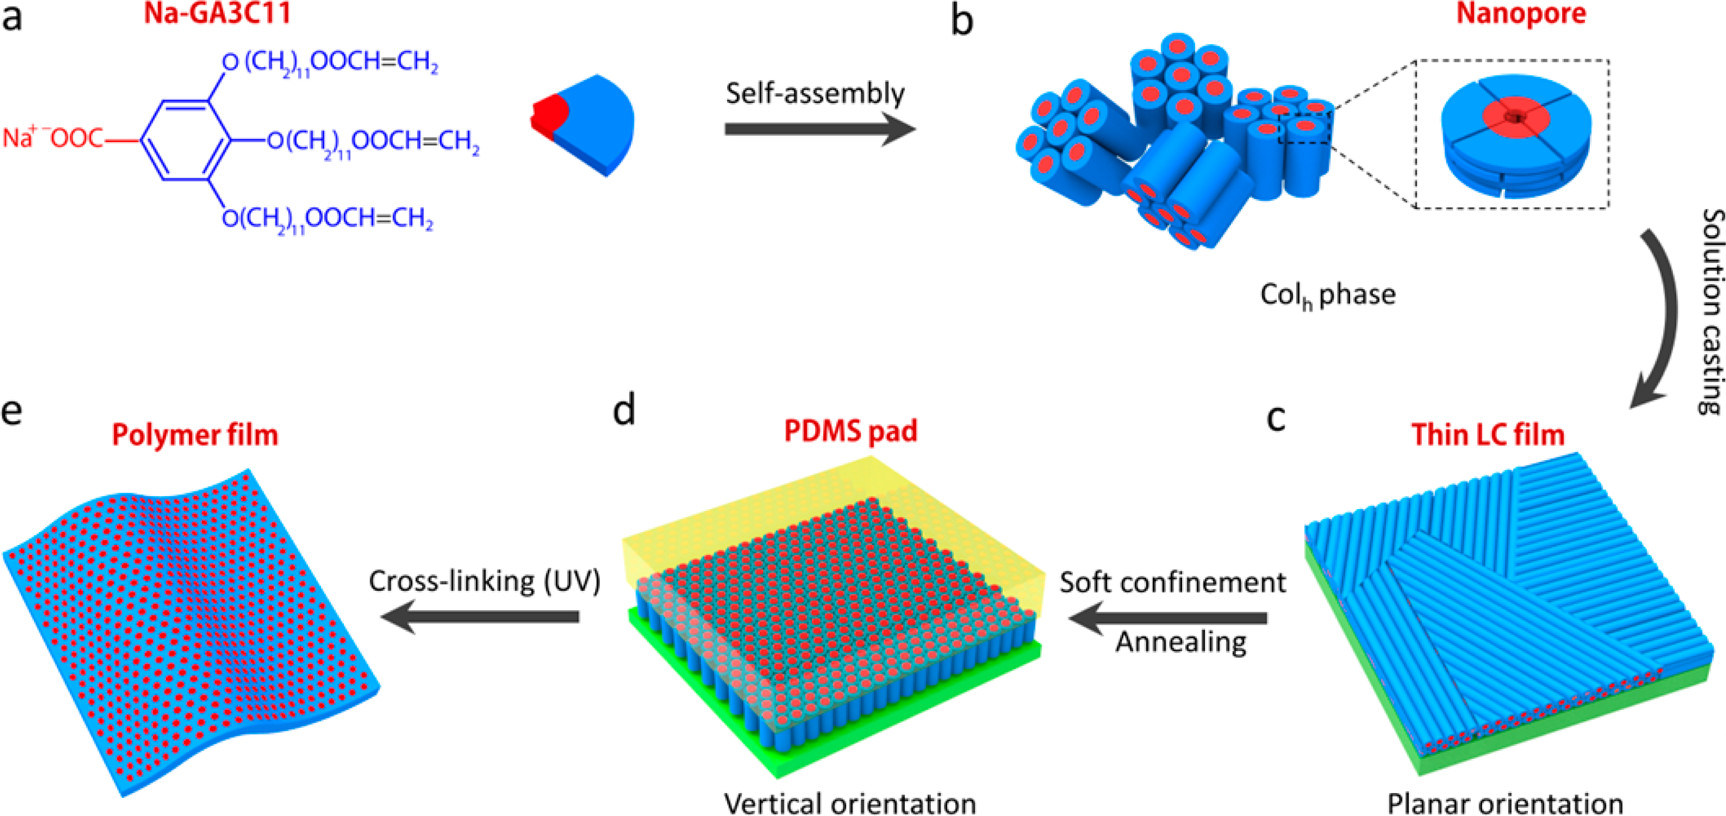
\includegraphics[width=\linewidth]{soft_confinement.png} \caption{The wedge
  %	  shaped liquid crystal monomer (a) self assembles into mesophases with
%		  hexagonally packed pores (b). The pores are made of stacked monomer disks. A
%		  sub-micron-thick film is created by casting a dilute solution of Na-GA3C11/THF
%		  solution onto a silicon substrate and and allowing the solvent to evaporate.
%		  The thin film contains nanoporous columns which lie parallel to the film plane.
%		  (d) When a soft PDMS pad is imposed to the thin film, with subsequent thermal
%		  annealing, the columns align perpendicular to the film plane. (e)
%		  Photo-cross-linking of the aligned film creates a mechanically stable thin film
%		  with vertically aligned nanopores}~\label{fig:soft} \end{figure}

  %BJC: Made my own version of the above, leaving out alignment details since it'

  \begin{figure}
	\centering
	\begin{subfigure}{.3\textwidth}
		\centering
		%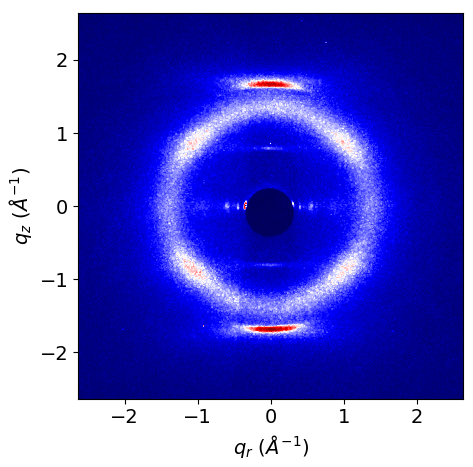
\includegraphics[width=\linewidth, trim={2.5cm 0 4cm 1.25cm}, clip]{WAXS_raw.png}
		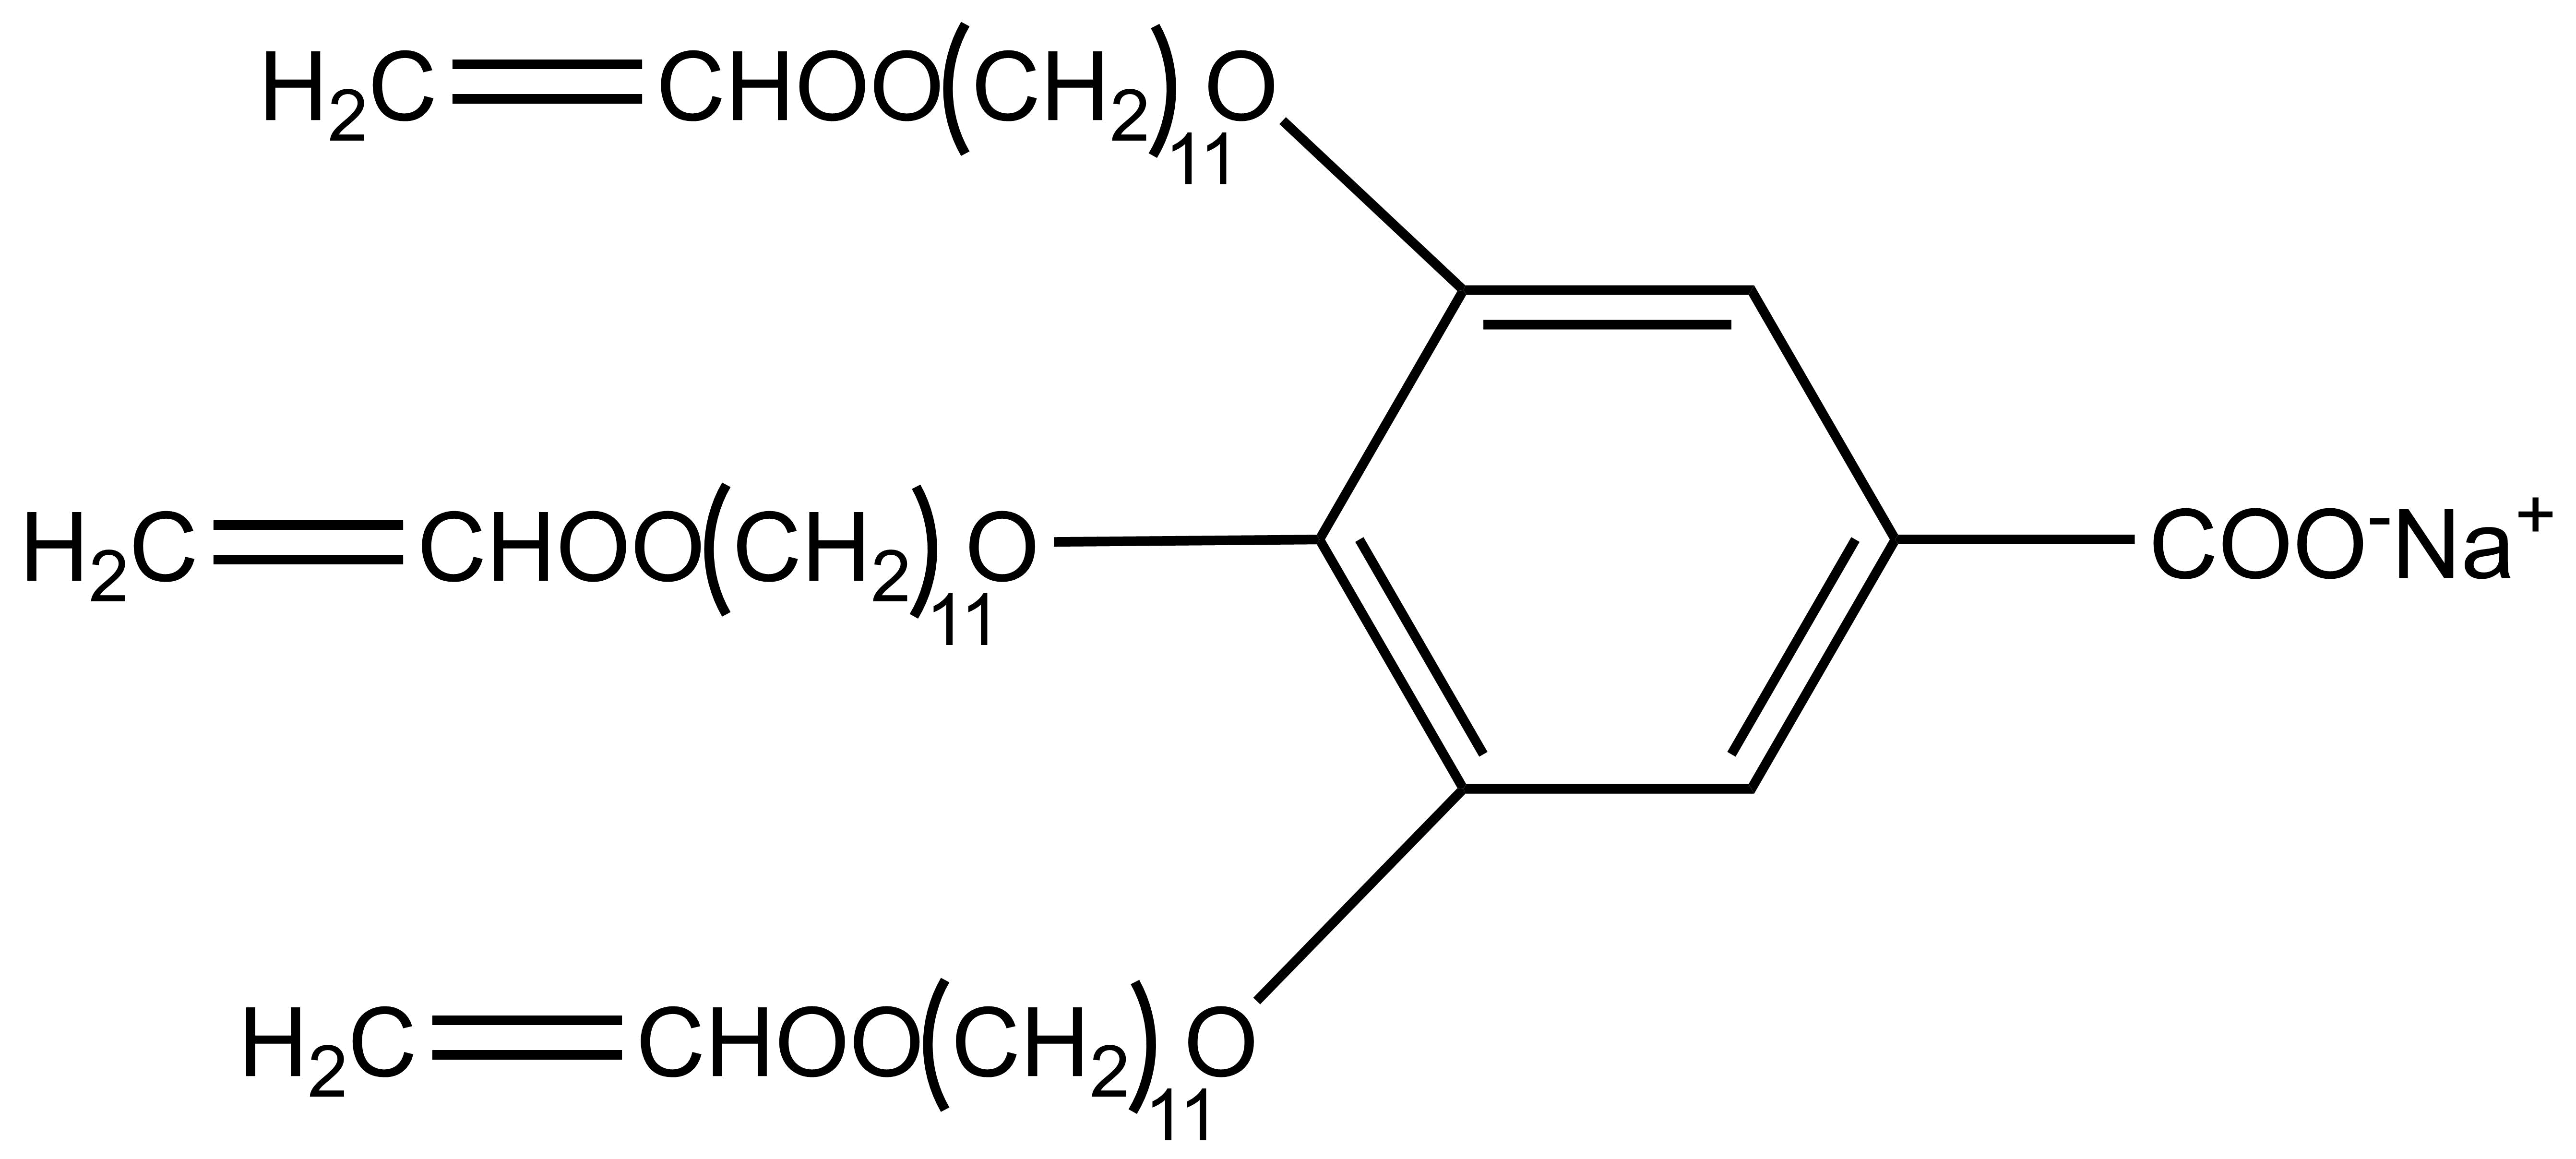
\includegraphics[width=\textwidth]{NaGA3C11.png}
		\caption{}~\label{fig:monomer}
	\end{subfigure}
	\begin{subfigure}{.3\textwidth}
		\centering
		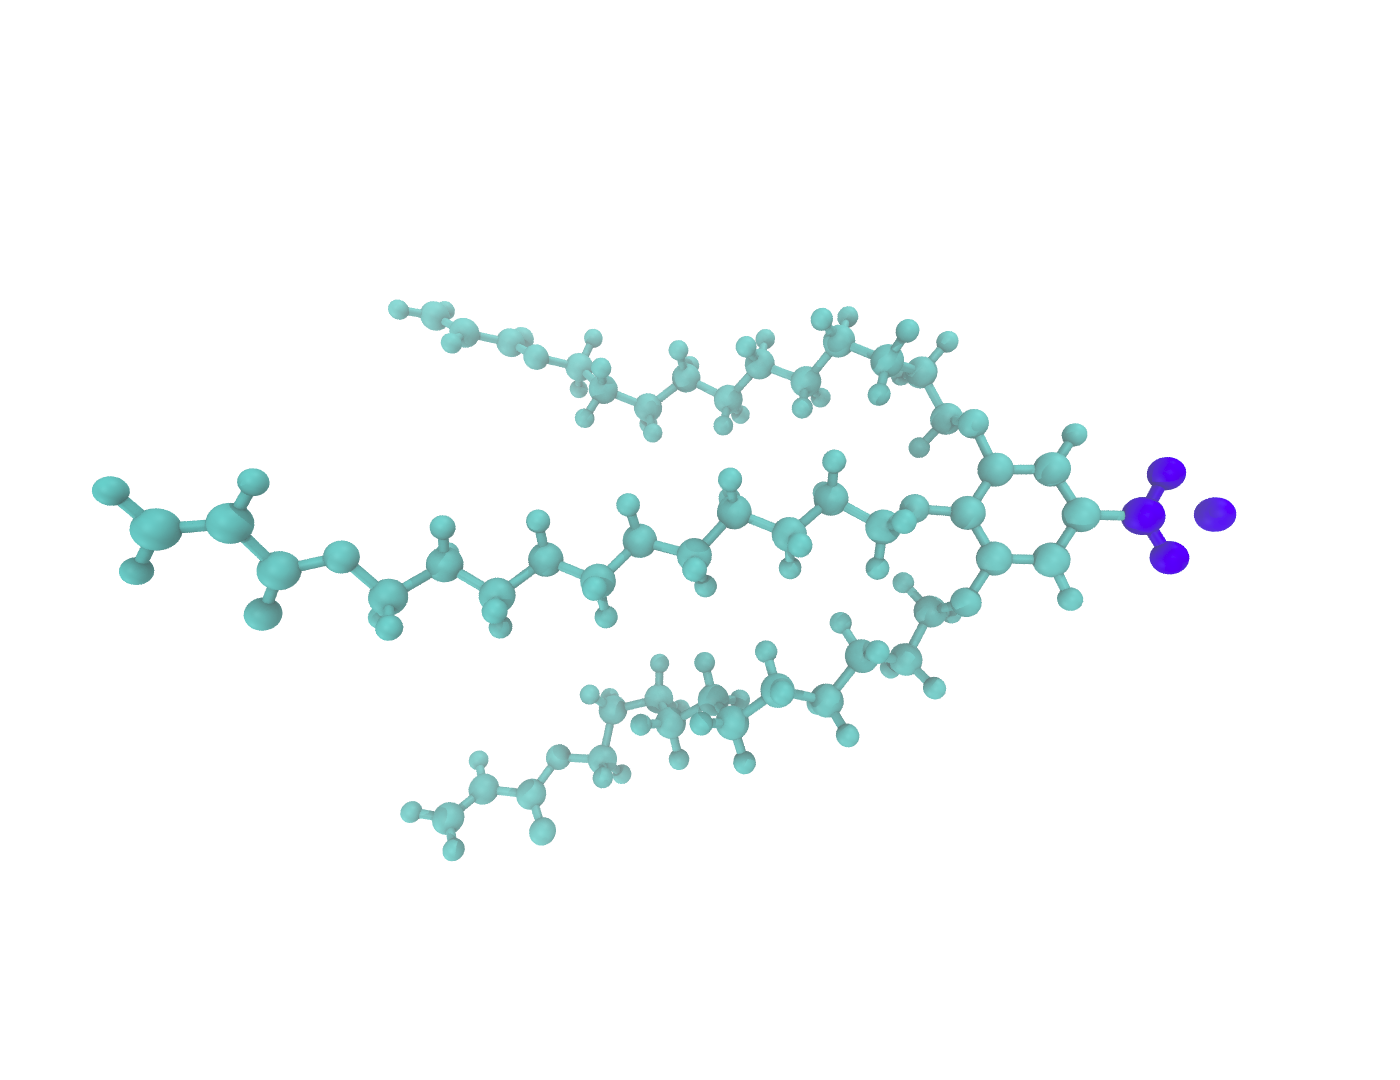
\includegraphics[width=\textwidth]{monomer_twocolor.png}
		\caption{}~\label{fig:atomistic_monomer}
	\end{subfigure}
	\begin{subfigure}{0.3\linewidth}
		\centering
		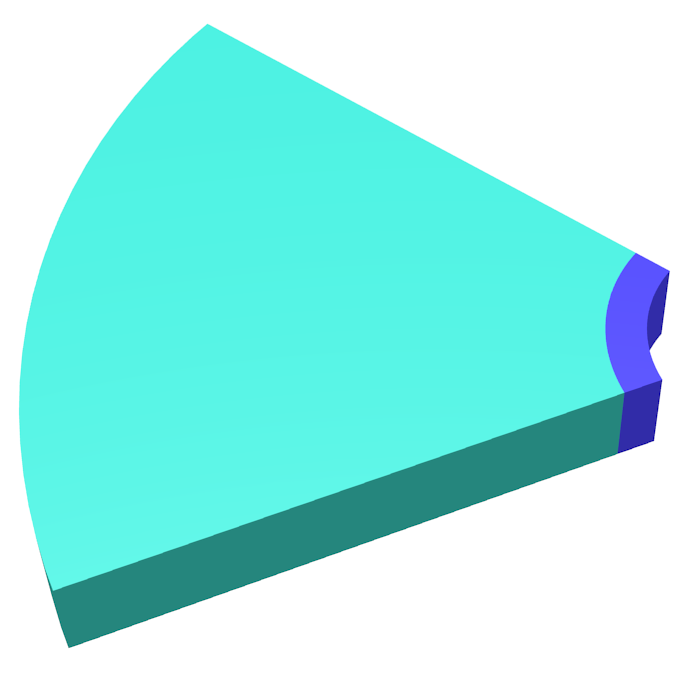
\includegraphics[width=\textwidth]{wedge.png}
		\caption{}~\label{fig:wedge}
	\end{subfigure}
		\begin{subfigure}{0.4\linewidth}
		\centering
		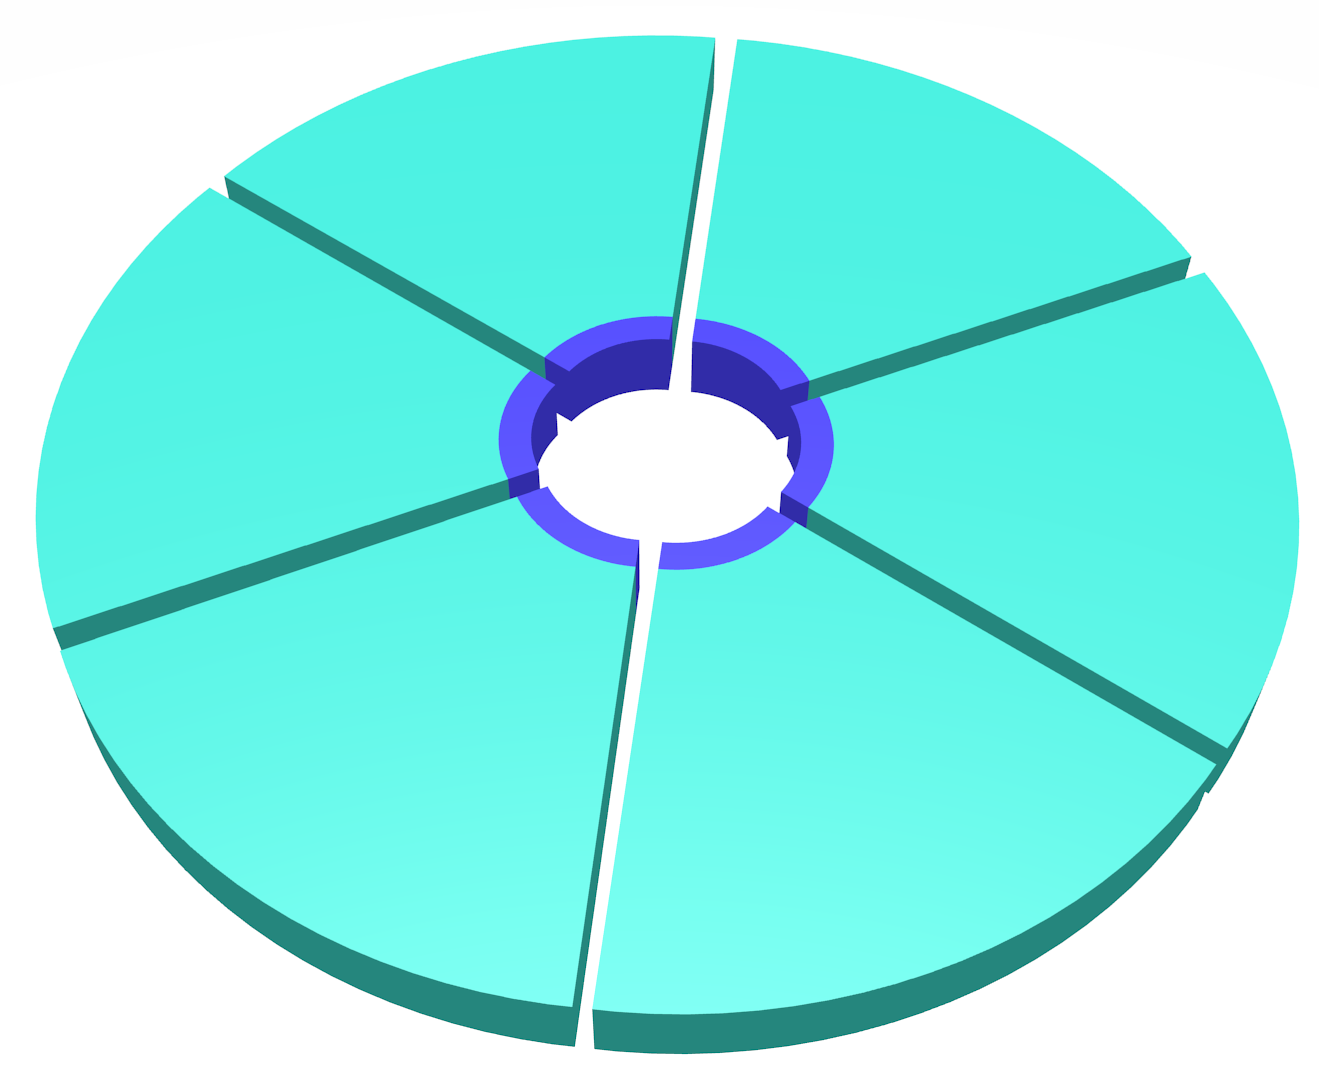
\includegraphics[width=\textwidth]{layer_blender.png}
		\caption{}~\label{fig:wedge_layer}
	\end{subfigure}
	\begin{subfigure}{0.4\linewidth}
		\centering
		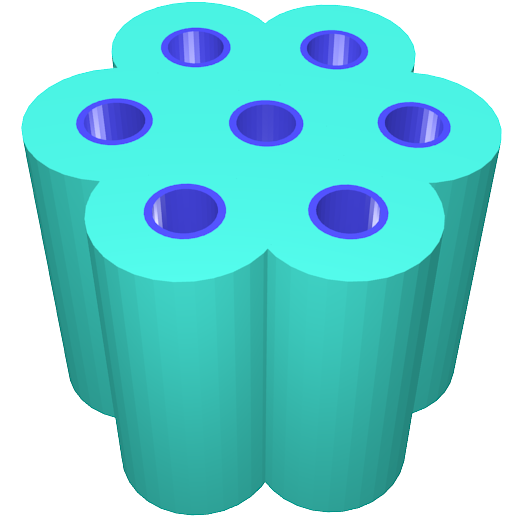
\includegraphics[width=\textwidth]{hexagonal_packing.png}
		\caption{}~\label{fig:hex_packing_simple}
	\end{subfigure}
	\caption{The liquid crystal monomer Na-GA3C11 (a) rendered atomistically (b)
	exhibits wedge-like character (c). Monomer wedges assemble into disks (d) with
	hydrophilic head groups (blue) facing towards the disk center. The disks
	assemble into hexagonally packed columnnar mesophases (e)}~\label{fig:assembly}
  \end{figure}

  Our current understanding of LLC systems is not rich enough to be able to
  precisely design membranes for specific separations. Over the past 20 years,
  H\textsubscript{II} phase LLC membrane studies have been limited primarily to
  Na-GA3C11 with some characterization done after minor structural modifications.
  Resel et al. varied the length of the monomer tails and the counterion used and
  observed its affect on pore spacing \cite{resel_structural_2000}.  Their study
  offers no insight into dynamics within the pore. Rejection studies show that
  membranes formed by NA-GA3C11 can not perform separations of solutes less than
  1.2 nm in diameter because the pores are too large \cite{zhou_supported_2005}.
  We do not yet understand how to controllably reduce the effective pore size or
  how to tune the chemical environment in the nanopores for effective water
  desalination or small organic molecule separations. The only source of
  predictive modeling for LLC systems have been macroscopic models which likely
  do not adequately describe transport at these length scales.
  \cite{hatakeyama_water_2011} It will be challenging to efficiently narrow down
  the large design space in a laboratory setting without a robust model.

  A molecular level understanding of LLC membrane structure, enabled by
  molecular dynamics simulations, will provide guidelines to reduce the large
  chemical space available to design monomers for creation of separation-specific
  membranes. A good molecular model should incorporate a detailed picture of the
  nanoscopic pore structure which will be crucial to understanding the role of
  monomer structure in solute transport and membrane design. Models resulting
  from molecular dynamics simulations will provide the required level of detail.
  We can directly observe solute transport and suggest governing mechanisms. We
  can observe how the choice of head group may influence pore size for size
  exclusion driven separations. We can interchange counterions which may
  influence both the pore size and the strength of the Donnan potential which
  affects the degree to which the membrane can exclude charged species. 

  % BJC: improve this figure
  \begin{figure}
  \centering
	\begin{subfigure}{0.45\linewidth}
		\centering
		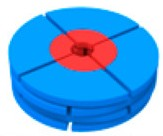
\includegraphics[width=\textwidth]{nanopore_undetailed.jpg}
		\caption{}~\label{fig:undetailed_pore}
	\end{subfigure}
	\begin{subfigure}{0.45\linewidth}
		\centering
		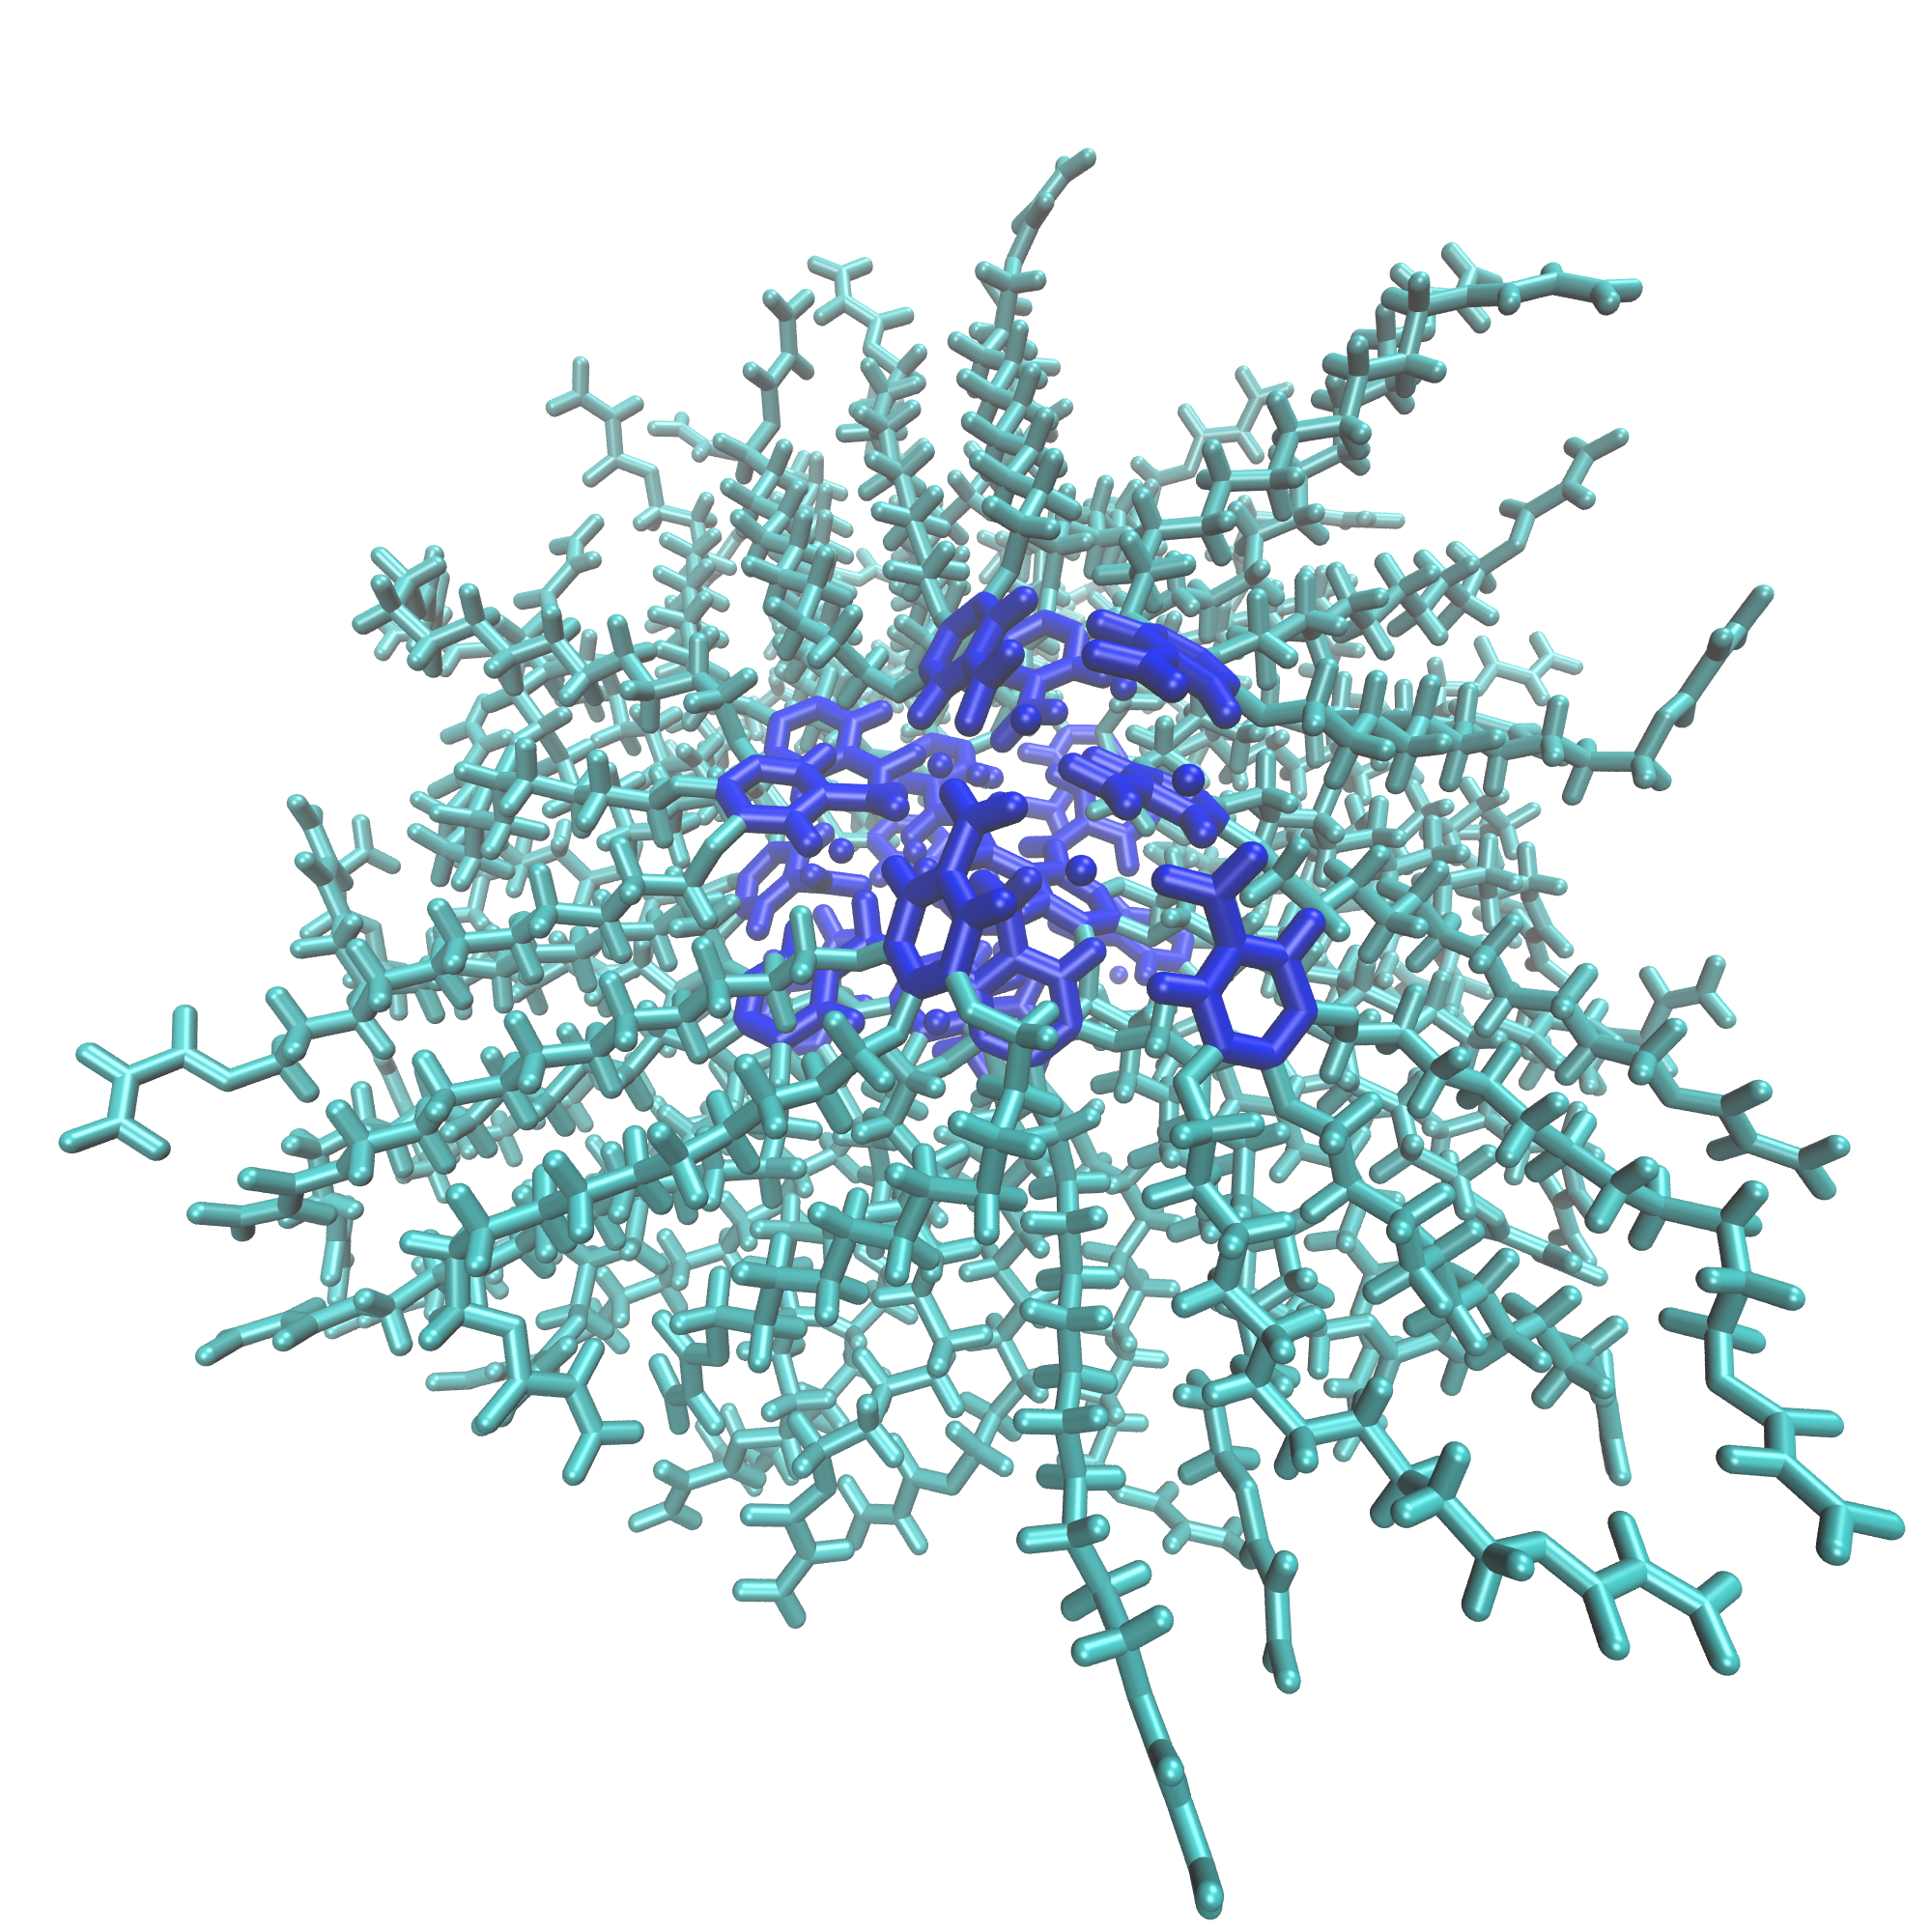
\includegraphics[width=\textwidth]{detailed_pore.png}
		\caption{}~\label{fig:detailed_pore}
	\end{subfigure}
  \caption{(a) Our previous understanding of the pore structure allows us to speculate
	   about separation behavior. (b) A detailed molecular model will allow us to
	   directly observe solute transport. Here, four stacked layers of 5 monomers
           are pictured atomistically. The hydrophilic region is in red and the 
	   hydrophoic region is colored blue.}~\label{fig:detail}
  \end{figure}
 
  %BJC: I think the first sentence of the following paragraph is
  %necessary to put somewhere, but maybe not in this spot exactly
  In order to appropriately model transport, we must gain a thorough
  understanding of the nanoscopic structure of LLC membranes.  Our approach to
  constructing a general model will follow the development of a model of the
  assembly formed by Na-GA3C11 since it has sufficient experimental
  characterization. We have also narrowed our scope to the development of a model
  of the Col\textsubscript{h} phase membrane. Compared to the H\textsubscript{II}
  phase, the Col\textsubscript{h} phase is a simpler starting point, due to the
  absence of water, and has detailed experimental Wide-angle X-ray scattering
  (WAXS) patterns useful for reconstructing structural data.  

  Despite having structural data, there is still information which experiment
  cannot definitively answer. There are several key questions that we will
  investigate which will be laid out and numbered in subsequent paragraphs.

  %BJC: commenting out :There has been no definitive answer in literature
  %regarding the number of monomers in each layer.  MRS3: the intro to the list
  %talks about only ``numbers of monomers in each layer'', whereas the list
  %below talks about several questions relating to layers. Can you rephrase so
  %it's more general? Maybe just take out that sentence above.

  Monomers in the Col\textsubscript{h} system are theorized to be partitioned
  into stacked layers which form columnar pores. We want to know 

  \begin{enumerate}

  \item If layers do exist, how many monomers constitute a single layer? \label{point:monomernum}
  
  A simple molecular simulation study of a similar molecule suggested that
  there are 4 monomers in each layer. Their estimation is based on a simulated
  system containing only 16 total monomers which likely does not sufficiently
  model the chemical environment present in the real system.
  \cite{zhu_methacrylated_2006}.  A separate calculation based on the volume of
  the liquid crystal monomers proposes that there are seven monomers in each
  layer \cite{resel_structural_2000}.  A molecular model orders of magnitude
  larger than any other reported atomistic liquid crystal membrane simulations
  has the best chance of directly answering this question.  We will directly
  change the layer composition and note its effect on membrane structure.

 \item Does our model support the existence of layers and if so, how well
 defined are the layers? \label{point:layers} 

  Experimentally, their existence is supported by evidence of strong $\pi$-$\pi$
  stacking interactions in the direction perpendicular to the membrane plane.
  $\pi$-$\pi$ stacking will only occur between the aromatic monomer head groups
  which leaves no description of what is happening in the monomer tail region.
  The tails may entangle isotropically while stacking order is maintained among
  headgroups. 

  \item How do monomers in each layer position themselves with respect to
  surrounding layers? \label{point:orientation}

  The $\pi$-$\pi$ stacking interactions may be a driving force of self assembly
  in this system. \cite{gazit_possible_2002} Gas phase ab initio studies of
  benzene dimers have shown a clear energetic advantage for parallel displaced
  and T-shaped $\pi$-$\pi$ stacking conformations versus a sandwiched
  conformation ~\cite{sinnokrot_estimates_2002}. Substituted benzene rings
  exhibit an even stronger $\pi$-$\pi$ stacking attraction which favors the
  parallel displaced configuration in all cases except where the substitutions
  are extremely electron withdrawing.
  \cite{waller_hybrid_2006,ringer_effect_2006}. We can use simulated X-ray
  diffration patterns to compare the two stacking configurations. 

  \item Can the system exist in other metastable states or phases that are not
  accessed during experiments? \label{point:metastable}
  
  There remains the possibility that there is more than one metastable state
  associated with a given LLC system. Simulating a membrane atomistically will
  require many atoms which limits the timescales acessible with MD. It is
  reasonable to expect that we will generate configurations which are kinetically
  trapped in a metastable free energy basin. We must be able to identify which
  state is produced experimentally and why others are not.

  \item What constitutes a pore and how well-defined are the pore regions? \label{point:poredefinition}

  The limited picture that experiment provides tells us that there are
  hexagonally packed, hydrophilic regions where transport is likely to occur.
  One may instinctively assume that these regions are tube-like pathways. We will
  explore the composition of the pores and the partition between the
  hydrophilic and hydrophobic regions. 

  \item Is it necessary to include any water in order to appropriately model
  the Col\textsubscript{h} phase? \label{point:water}

  While the Col\textsubscript{h} phase is described as dry, it is has been
  suggested by experimentalists in unpublished communications that it is likely
  that small amounts of ambient water are leached into neat monomer.
  Experimentally, achieving a hexagonal phase with a completely dry system has
  proven difficult. If neat monomer is allowed to sit in ambient conditions, its
  color turns from transparent to slightly opaque and a hexagonal phase forms.
  Although we will not explore whether water is necessary for self assembly, we
  hypothesize that the hydrogen bonding network formed by the water may play a
  role in structuring the pores and holding together the hexagonal phase. We can
  use simulated X-ray diffraction patterns to see if there is any meaningful
  structural difference between a "dry" and "wet" system.

  \end{enumerate}
  
  %Once we have addressed all of the above questions, we must show that the 
  %developed molecular model is consistent with physical observations so that we
  %can rely on conclusions drawn about structural features characteristic of 
  %the system.
 
  In this study, we build a significantly more realistic atomistic model of LLC
  membranes than, to our knowledge, has ever previously been done, and explore
  what new structural information can be gained and what structure hypotheses are
  supported by this model. We validate the model using as much experimental
  information as possible. We are most interested in reproducing the conclusions
  about structure which have been drawn from X-ray diffraction (XRD) experiments
  and in matching ionic conductivity measurements \cite{feng_thin_2016}.

  %BJC: Would it be better to describe each reflection as a numbered list (like with the questions above?)
  We used experimental wide angle X-ray scattering (WAXS) data (produced as 
  described in \cite{feng_scalable_2014}) and small-angle X-ray scattering (SAXS)
  data from \cite{feng_thin_2016} to inform our choices of some initial
  structural parameters (Figure~\ref{fig:SWAXS}). We rely primarily on the 2D
  WAXS data since it encodes all structural details down to the sub-nm scale.
  There are five major features of interest present in the 2D experimental
  pattern shown in Figure \ref{fig:WAXS}. The first is located at $q_z$ = 1.7
  \angstrom$^{-1}$, corresponding to a real space separation of 3.7 \angstrom~.
  The reflection is attributed to $\pi$-$\pi$ stacking between aromatic rings in
  the direction perpendicular to the membrane plane, or z-axis
  \cite{feng_scalable_2014}. For simplicity, this reflection will be referred to
  as R-$\pi$. A weak intensity line is located at exactly half the $q_z$ value of
  R-$\pi$ ($q_z$ = 0.85 \angstrom$^-1$), corresponding to a real space periodic
  spacing of 7.4 \angstrom~. This reflection has been interpreted as
  2\textsubscript{1} helical ordering of aromatic rings along the z axis meaning
  if the positions of the aromatic rings can be traced by a helix, then for each
  turn in the helix, there should be two aromatic rings. For this reason it will
  be referred to as R-helix. A third major reflection is marked by a low
  intensity ring located at r = 1.4 \angstrom$^-1$. The real space separation
  corresponds to 4.5 \angstrom~ which is characteristic of the average spacing
  between packed alkane chains. This reflection will be called R-alkanes. Within
  R-alkanes, are four spots of higher relative intensity which will be called
  R-spots. All are located $\approx 40$ degrees from the $q_z$ axis in their
  respective quadrants. In many liquid crystal systems this can be explained by
  the tilt angle of the alkane chains with respect to the xy plane.  The final
  feature corresponds to the spacing and symmetry of the d\textsubscript{100}
  plane which can be related to the distance between pores.  The feature, which
  will be called R-pores, is characterized by dots along $q_z$ = 0. The spacing
  between dots is indicative of the hexagonal symmetry of the packed pores. The
  same information at higher resolution is obtained using a SAXS setup. By
  radially integrating the 2D data one gets a 1D curve which is shown in
  Figure~\ref{fig:SAXS}.

  \begin{figure}
        \centering
        \begin{subfigure}[t]{0.43\linewidth}
                \centering
        %       \vspace{12mm}
                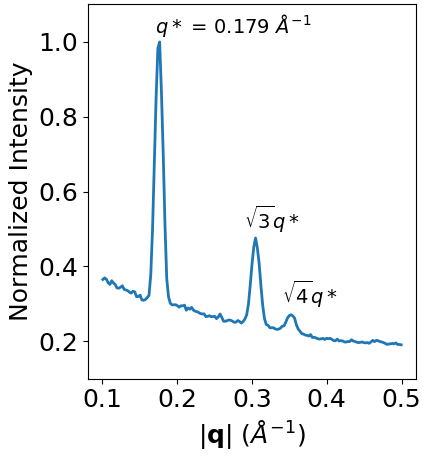
\includegraphics[width=\linewidth]{SAXS.png}
                \caption{}\label{fig:SAXS}
        \end{subfigure}
        \begin{subfigure}[t]{0.47\linewidth}
                \centering
                \raisebox{.2\textwidth}{%
                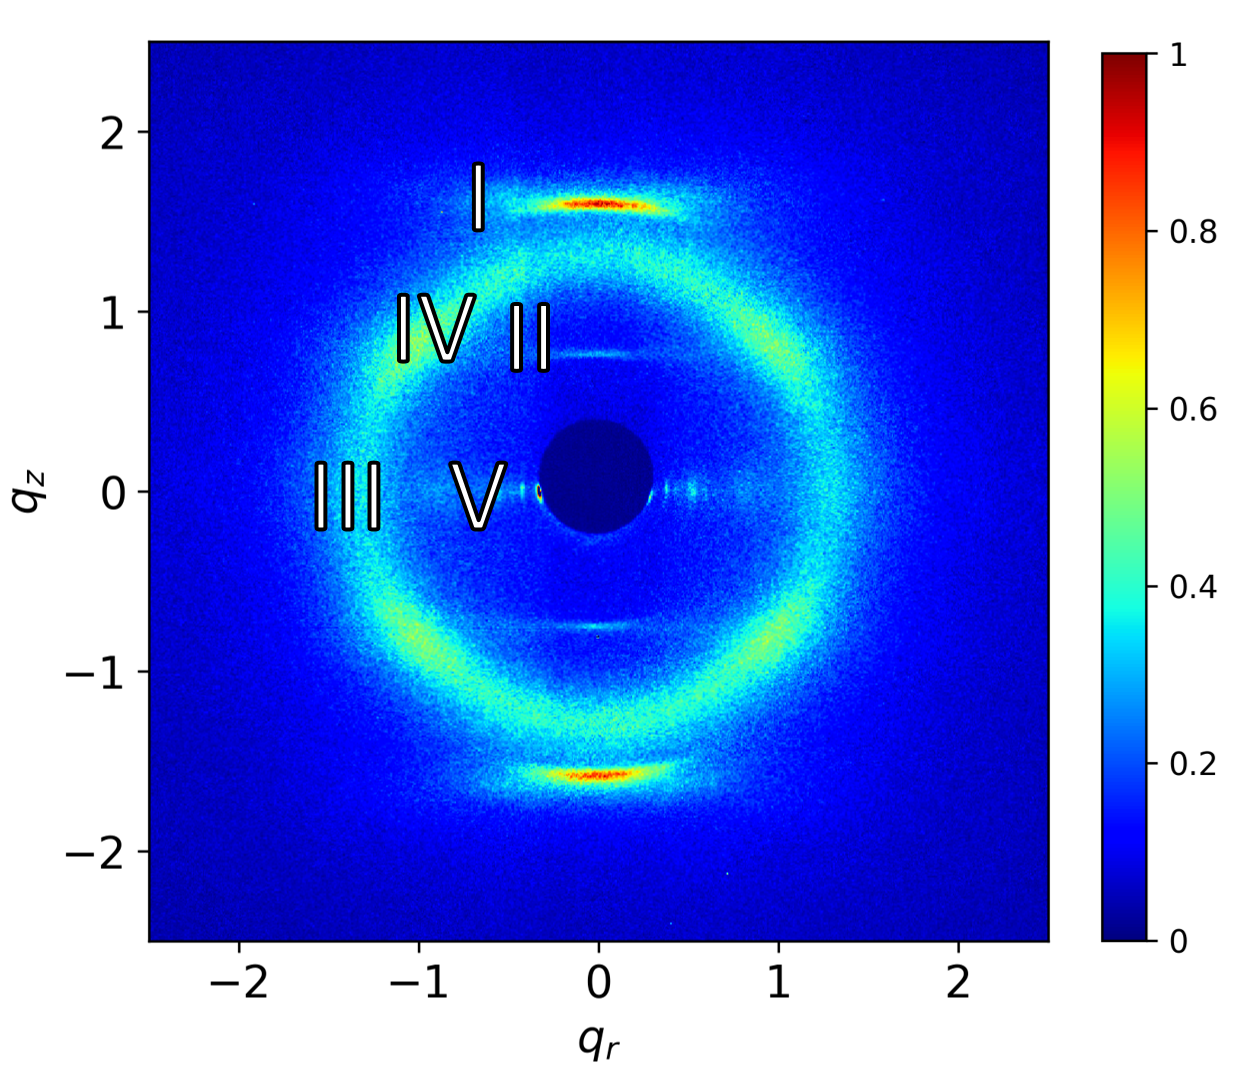
\includegraphics[width=\linewidth]{WAXS_annotated.png}
                }
                \caption{}\label{fig:WAXS}
        \end{subfigure}
        \caption{(a) 1D small angle X-ray scattering indicates hexagonal packing of
        pores as well as the spacing between pores (b) 2D wide angle X-ray scattering
        gives details about repeating features less than 1 nanometer apart}\label{fig:SWAXS}
  \end{figure}

  \section*{Methods}
 
  \subsection*{Monomer Placement}

  Liquid crystal monomers were parameterized using the Generalized AMBER
  Forcefield \cite{wang_development_2004} with the Antechamber package
  \cite{wang_automatic_2006} provided with AmberTools16
  \cite{case_ambertools16_2016}. Atomic charges were assigned using the am1bccsym
  method of molcharge shipped with QUACPAC from Openeye Scientific Software. All
  molecular dynamics simulations were run using Gromacs 2016.
  \cite{bekker_gromacs:_1993,berendsen_gromacs:_1995,van_der_spoel_gromacs:_2005,hess_gromacs_2008}

  An ensemble of characteristic, low-energy vacuum monomer configurations
  were constructed by applying a simulated annealing process to a parameterized
  monomer. Monomers were cooled from 1000K to 50K over 10 nanoseconds.  A low
  energy configuration was randomly pulled from the trajectory and charges were
  reassigned using molcharge.  Using the new charges, the monomer system was
  annealed again and a random monomer configuration was pulled from the
  trajectory to be used for full system construction (Figure~\ref{fig:python}a).

  \subsection*{Unit Cell Preparation}

  The timescale for self assembly of monomers into the hexagonal phase is
  unknown and likely outside of a reasonable length for an atomistic
  simulation, calling for a more efficient way to build the system.  Previous
  work has shown a coarse grain model self assemble into the H\textsubscript{II}
  phase configuration in $\approx$ 1000 ns \cite{mondal_self-assembly_2013}.  We
  attempted atomistic self-assembly by packing monomers into a box using Packmol
  \cite{martinez_packmol:_2009}.  Simulations of greater than 100 ns show no
  indicators of progress towards an ordered system (See supplemental information
  for further details). To bypass the slow self-assembly process, python scripts
  are used to assemble monomers into a structure close to one of a number of
  hypothesized equilibrium configurations (Figure~\ref{fig:python}).

  \begin{figure}
	\centering
	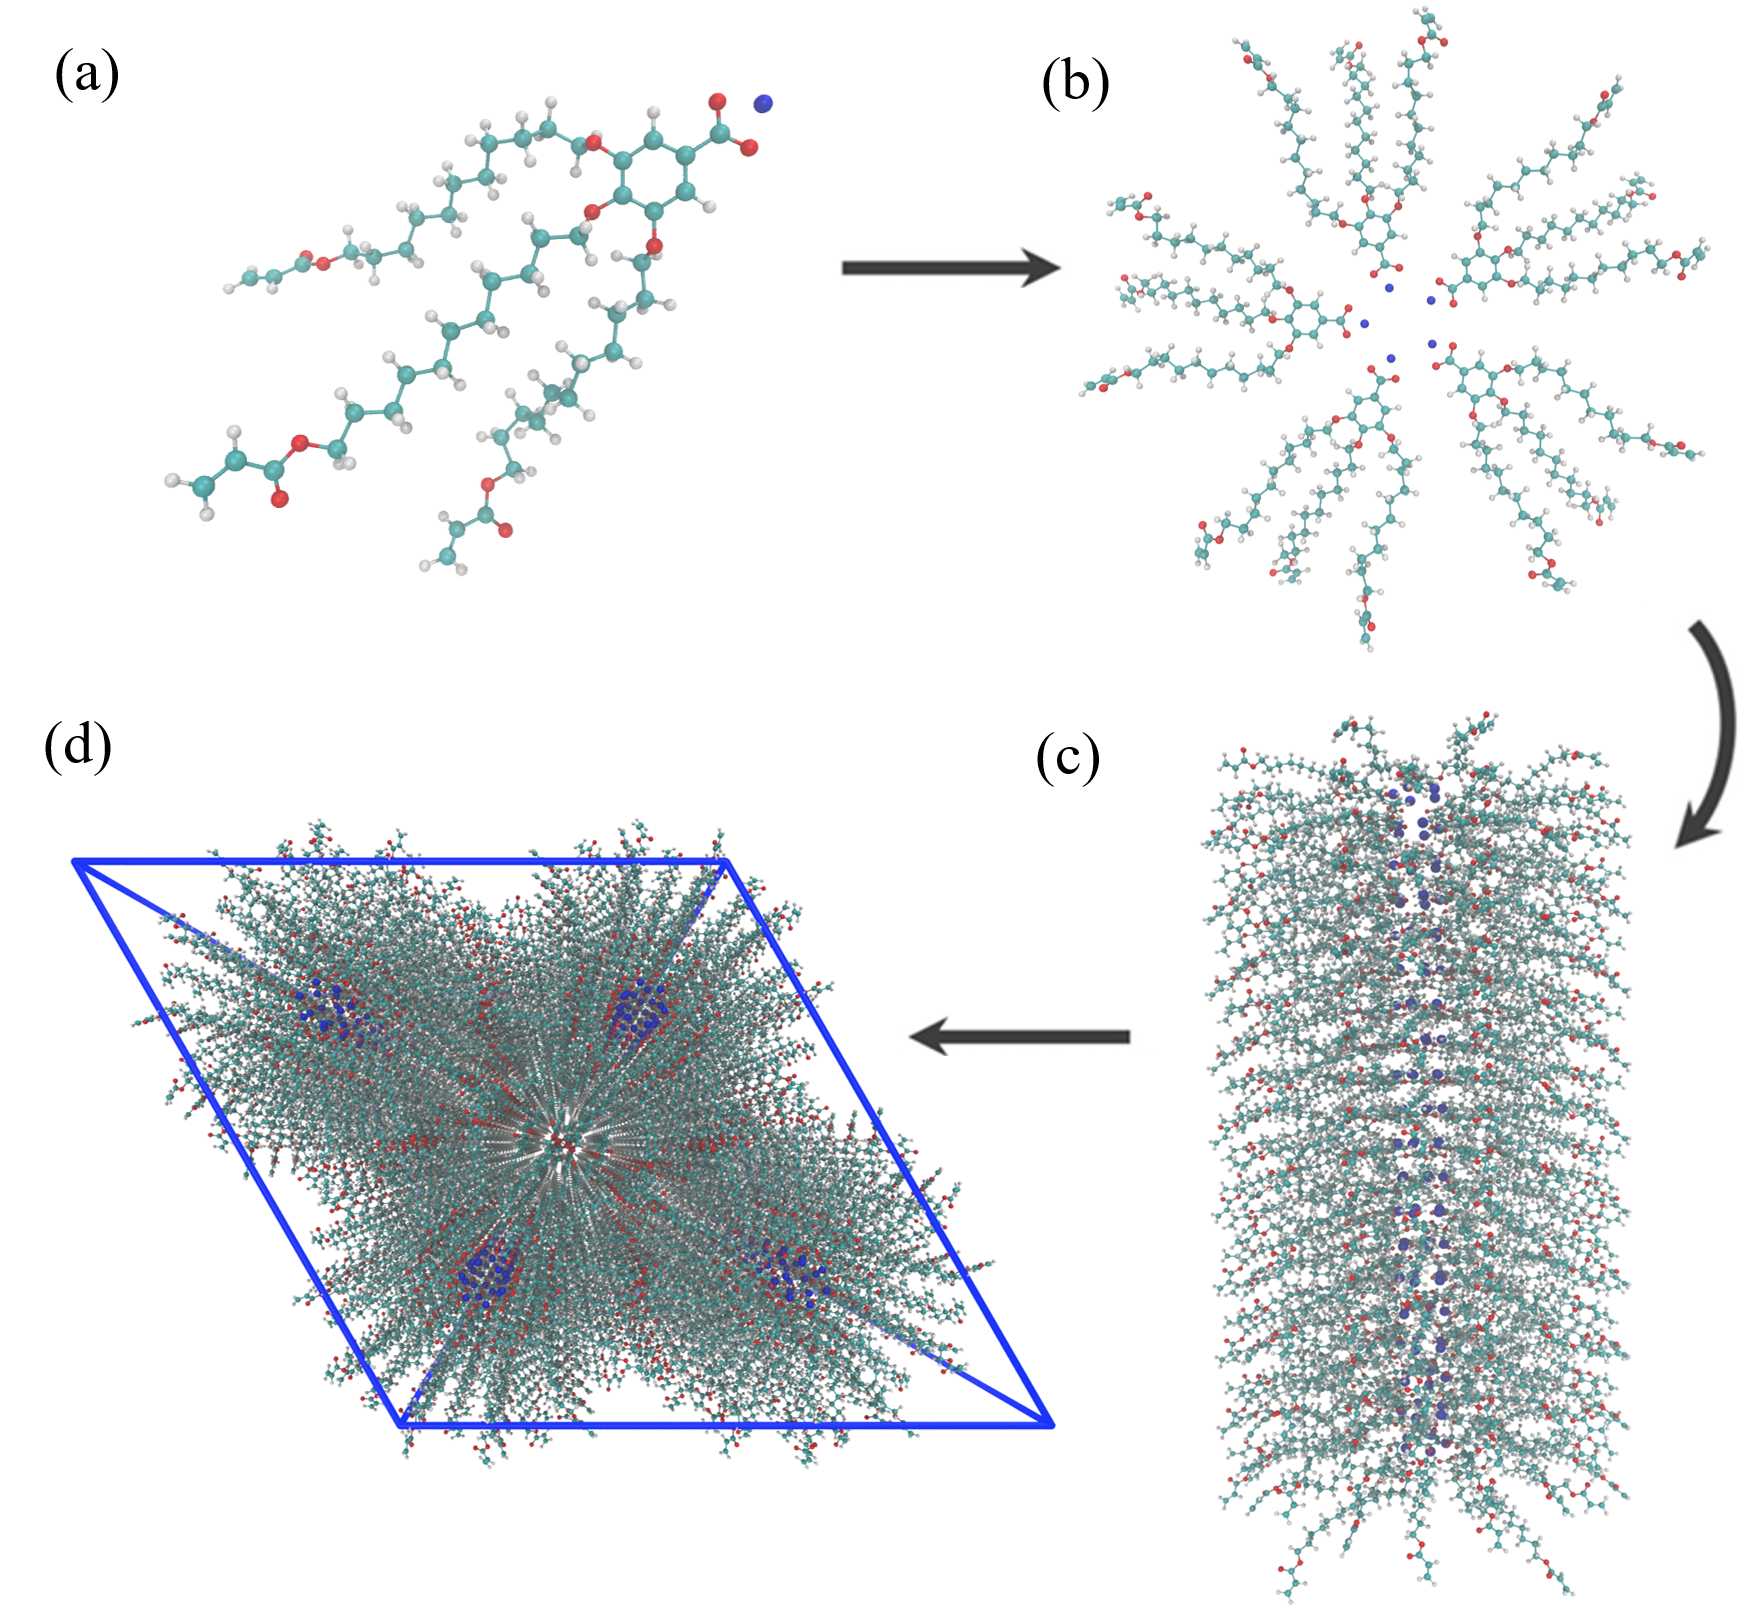
\includegraphics[width=0.75\linewidth]{build.PNG} %BJC: put an xyz axis with the unit cell
	\caption{(a) A single monomer was parameterized and annealed to produce a low energy
		configuration. (b) Monomers are rotated and assembled into layers with 
		hydrophlic centers. (c) Twenty layers are stacked on top of each other to create
		a pore. (d) Pores are duplicated and placed into a monoclinic unit cell}\label{fig:python}
  \end{figure}
  
  A typical simulation volume contains four pores in a monoclinic unit cell,
  the smallest unit cell that maintains hexagonal symmetry when extended
  periodically. Each pore is made of twenty stacked monomer layers with periodic
  continuity in the z direction, avoiding any edge effects and creating an
  infinite length pore ideal for studying transport. A small number of layers is
  preferred in order to reduce computational cost and to allow us to look at
  longer timescales. Ultimately, we chose to build a system with 20 monomer
  layers in each pore in order to obtain sufficient resolution when simulating
  X-ray diffraction patterns. This point will be explained in more detail later.

\subsection*{Monomer Placement} 

  When constructing an initial configuration, there are a number of variables
  which require careful consideration while placing monomers. The equilibrium
  configuration is sensitive to some while insensitive to others. The starting
  pore radius, defined as the distance of a chosen head group carbon from the
  pore's central axis, does not influence the equilibrium structure when a
  reasonable value is chosen (See Supplemental). The pore radius is chosen to be
  0.6 nm in our initial configurations because the pore size is estimated to be
  $\approx$ 1.2 nm. The initial distance between pores also has little effect on
  the the equilibrated structure. However, one should not start them too close or
  there will likely be unintended high energy repulsions during early
  equilibration. We chose an initial pore spacing of 4.5 nm, $\approx$ 10 \%
  larger than the experimental value of 4.12 nm.  The distance between layers,
  the rotation of the layers with respect to adjacent layers, and the number of
  monomers per layer do influence the equilibrium structure and require further
  justification for their choices. We rely on experimental data to inform our
  choices

  We chose the layer spacing for the initial configuration based on R-$\pi$ and
  then allowed system to readjust during equilibration. Each monomer was rotated
  so the plane of the aromatic head groups would be coplanar with the xy plane.
  We explore two different initial layer spacings. The first is exactly equal to
  R-$\pi$ with layers placed so aromatic rings are stacked 3.7 \angstrom~ apart
  in the z-direction.  A second system is explored with an initial layer spacing
  of 5 \angstrom. A third system with an initial layer spacing of 10 \angstrom was
  briefly explored. When layers are spaced out too far, they will collapse
  on each other while simultaneously slipping in between layers of adjacent pores
  which leads to an artificially thick membrane with pores spaced closely
  together. There will be no further discussion of this system but the interested
  reader can learn more about it in the supplemental information.

  The relative interlayer orientation was chosen based on clues from
  diffraction data as well as the various known stacking modes of benzene and
  substituted benzene rings: sandwiched, parallel-displaced and T-shaped
  ~\cite{sinnokrot_estimates_2002} (\Cref{fig:sandwiched,fig:pd,fig:tshaped}).
  The T-shaped configuration was ruled out because its $\approx$ 5 \angstrom
  equilibrium stacking distance ~\cite{sinnokrot_estimates_2002} is inconsistent
  with R-$\pi$. It is also unfeasible for the monomers to orient in the t-shaped
  conformation because of the bulky tail groups. The system's preference towards
  the sandwiched vs. parallel displaced stacking modes will be explored in some
  detail.  Both have reported stacking distances near the R-$\pi$ value of 3.7
  \angstrom. Headgroups in our sandwiched initial configuration are stacked
  directly on top of each other while stacked headgroups in the parallel
  displaced initial configuration are offset by $180/nmon$ degrees where $nmon$
  equals the number of monomers per layer.

  As outlined in \ref{point:monomernum} the number of monomers in each layer is
  unknown. We tested configurations constructed with a varied number of
  monomers per layer. Systems were built in the offset and parallel displaced
  configurations with 4, 5, 6, 7 and 8 monomers per layer.

  \subsection*{Equilibration}

  We developed equilibration schemes to create dry and wet configurations. Both
  schemes start with an initial configuration generated according to the previous
  guidelines. To create a dry configuration, we fix monomer head groups in the
  sandwiched or parallel-displaced configuration using position restraints with a
  force constant of 1e6 KJ mol$^-1$ nm$^-2$. We run a 50 ps simulation in the
  NVT ensemble which allows the monomer tails to settle without disrupting the
  ordering of the head groups. Doing so also mitigates system dependence on
  initial monomer configuration. Every 50 ps, we reduce the force constants by
  the square root of its previous value. Once the force constant is below 10 KJ
  mol$^-1$ nm$^-2$, the restraints are released linearly until there is no more
  restraining potential. The resulting unrestrained structure is allowed to
  equilibrate for 5 ns in the NPT ensemble with pressure controlled by the
  berendsen barostat. Next, we run a long NPT equilibration simulations for at
  least 400 ns using the Parrinello-Rahman barostat with a time consant of 10 ps.
  In order to create a wet system, we solvated an initial configuration with
  water using gmx solvate. All water molecules placed outside the pore region are
  removed. Waters inside the pore region are randomly removed until the desired
  concentration of water in the pores is reached. The remainder of the
  equilibration follows the same procedure as the dry system. In all cases, the
  v-rescale thermostat was used with tau-t = 0.1. % Supplemental

  \subsection*{Crosslinking}

  Using an equilibrated structure, we performed a crosslinking procedure
  in order to match synthetic procedures. The purpose of crosslinking
  is to maintain macroscopic alignment of the crystalline domains, 
  ensuring aligned, hexagonally packed pores. For that reason, we are not
  concerned with replicating the kinetics of the reaction, but instead emphasize
  the consistency of the final structure with experimental structural data. The
  algorithm was developed based on the known reaction mechanism. Crosslinking of
  this system is a free radical polymerization (FRP) taking place between
  terminal vinyl groups present on each of the three monomer tails. FRPs require
  an initiator which bonds to the system, meaning new atoms are introduced into
  the system. For simplicity, the initiator was simulated as hydrogen and made
  present in the simulation by including them in all possible locations where an 
  addition could occur as dummy atoms. The crosslinking procedure is carried out
  iteratively. During each iteration, bonding carbon atoms are chosen based on
  a distance cut-off. The topology is updated with new bonds and dummy hydrogen
  atoms are changed to appropriate hydrogen types. Head-to-tail addition was the
  only propagation mode considered due to its dominance in the real system.
  Direction of attack was not considered because the resultant mixture is
  racemic.

  \subsection*{Equilibrium Calculations}

  Using equilibrated structures, we carry out various calculations to
  characterize the system. We define the point at which a system is
  equilibrated based on when the distance between pores stops changing.

  To calculate the equilibrated pore spacing, we measured the distance between
  pore centers. Pore centers are located by averaging the coordinates of sodium
  ions in their respective pores. Pore spacing statistics were generated 
  using the bootstrapping technique (See Supplemental Information).

  To quantify the degree of layering and the equilibrium distance between layers
  in our system, we calculate a spatial correlation function, $g(z)$, measured
  along the z-axis (perpendicular to the membrane plane). To calculate $g(z)$,
  we binned the z-component distances between the center of mass of each
  component and all others of the same pore over at least 50 ns of equilibrated
  trajectory and then normalized by the average number density. To extract the
  average distance between layers we applied a discrete fourier transform to
  $g(z)$ and extracted the highest intensity frequency.

  % BJC: To be replaced by Joe's description
  Simulated X-ray diffraction patterns are generated based on atomic
  coordinates in order to make a direct experimental comparison. All atomic
  coordinates were simulated as gaussian spheres of electron density
  corresponding to each atom's atomic number. A three dimensional fourier
  transform (FT) of the array of electron density results in a three dimensional
  structure factor which represents the unit cell in reciprocal space. We matched
  experimental 2D WAXS patterns by adjusting the initial spacing between layers
  and the orientation of the head groups with respect to adjacent layers.

  % BJC: I think this figure belongs somewhere else
  \begin{figure}
	\centering
	\begin{subfigure}[b]{0.32\textwidth}
		\centering
		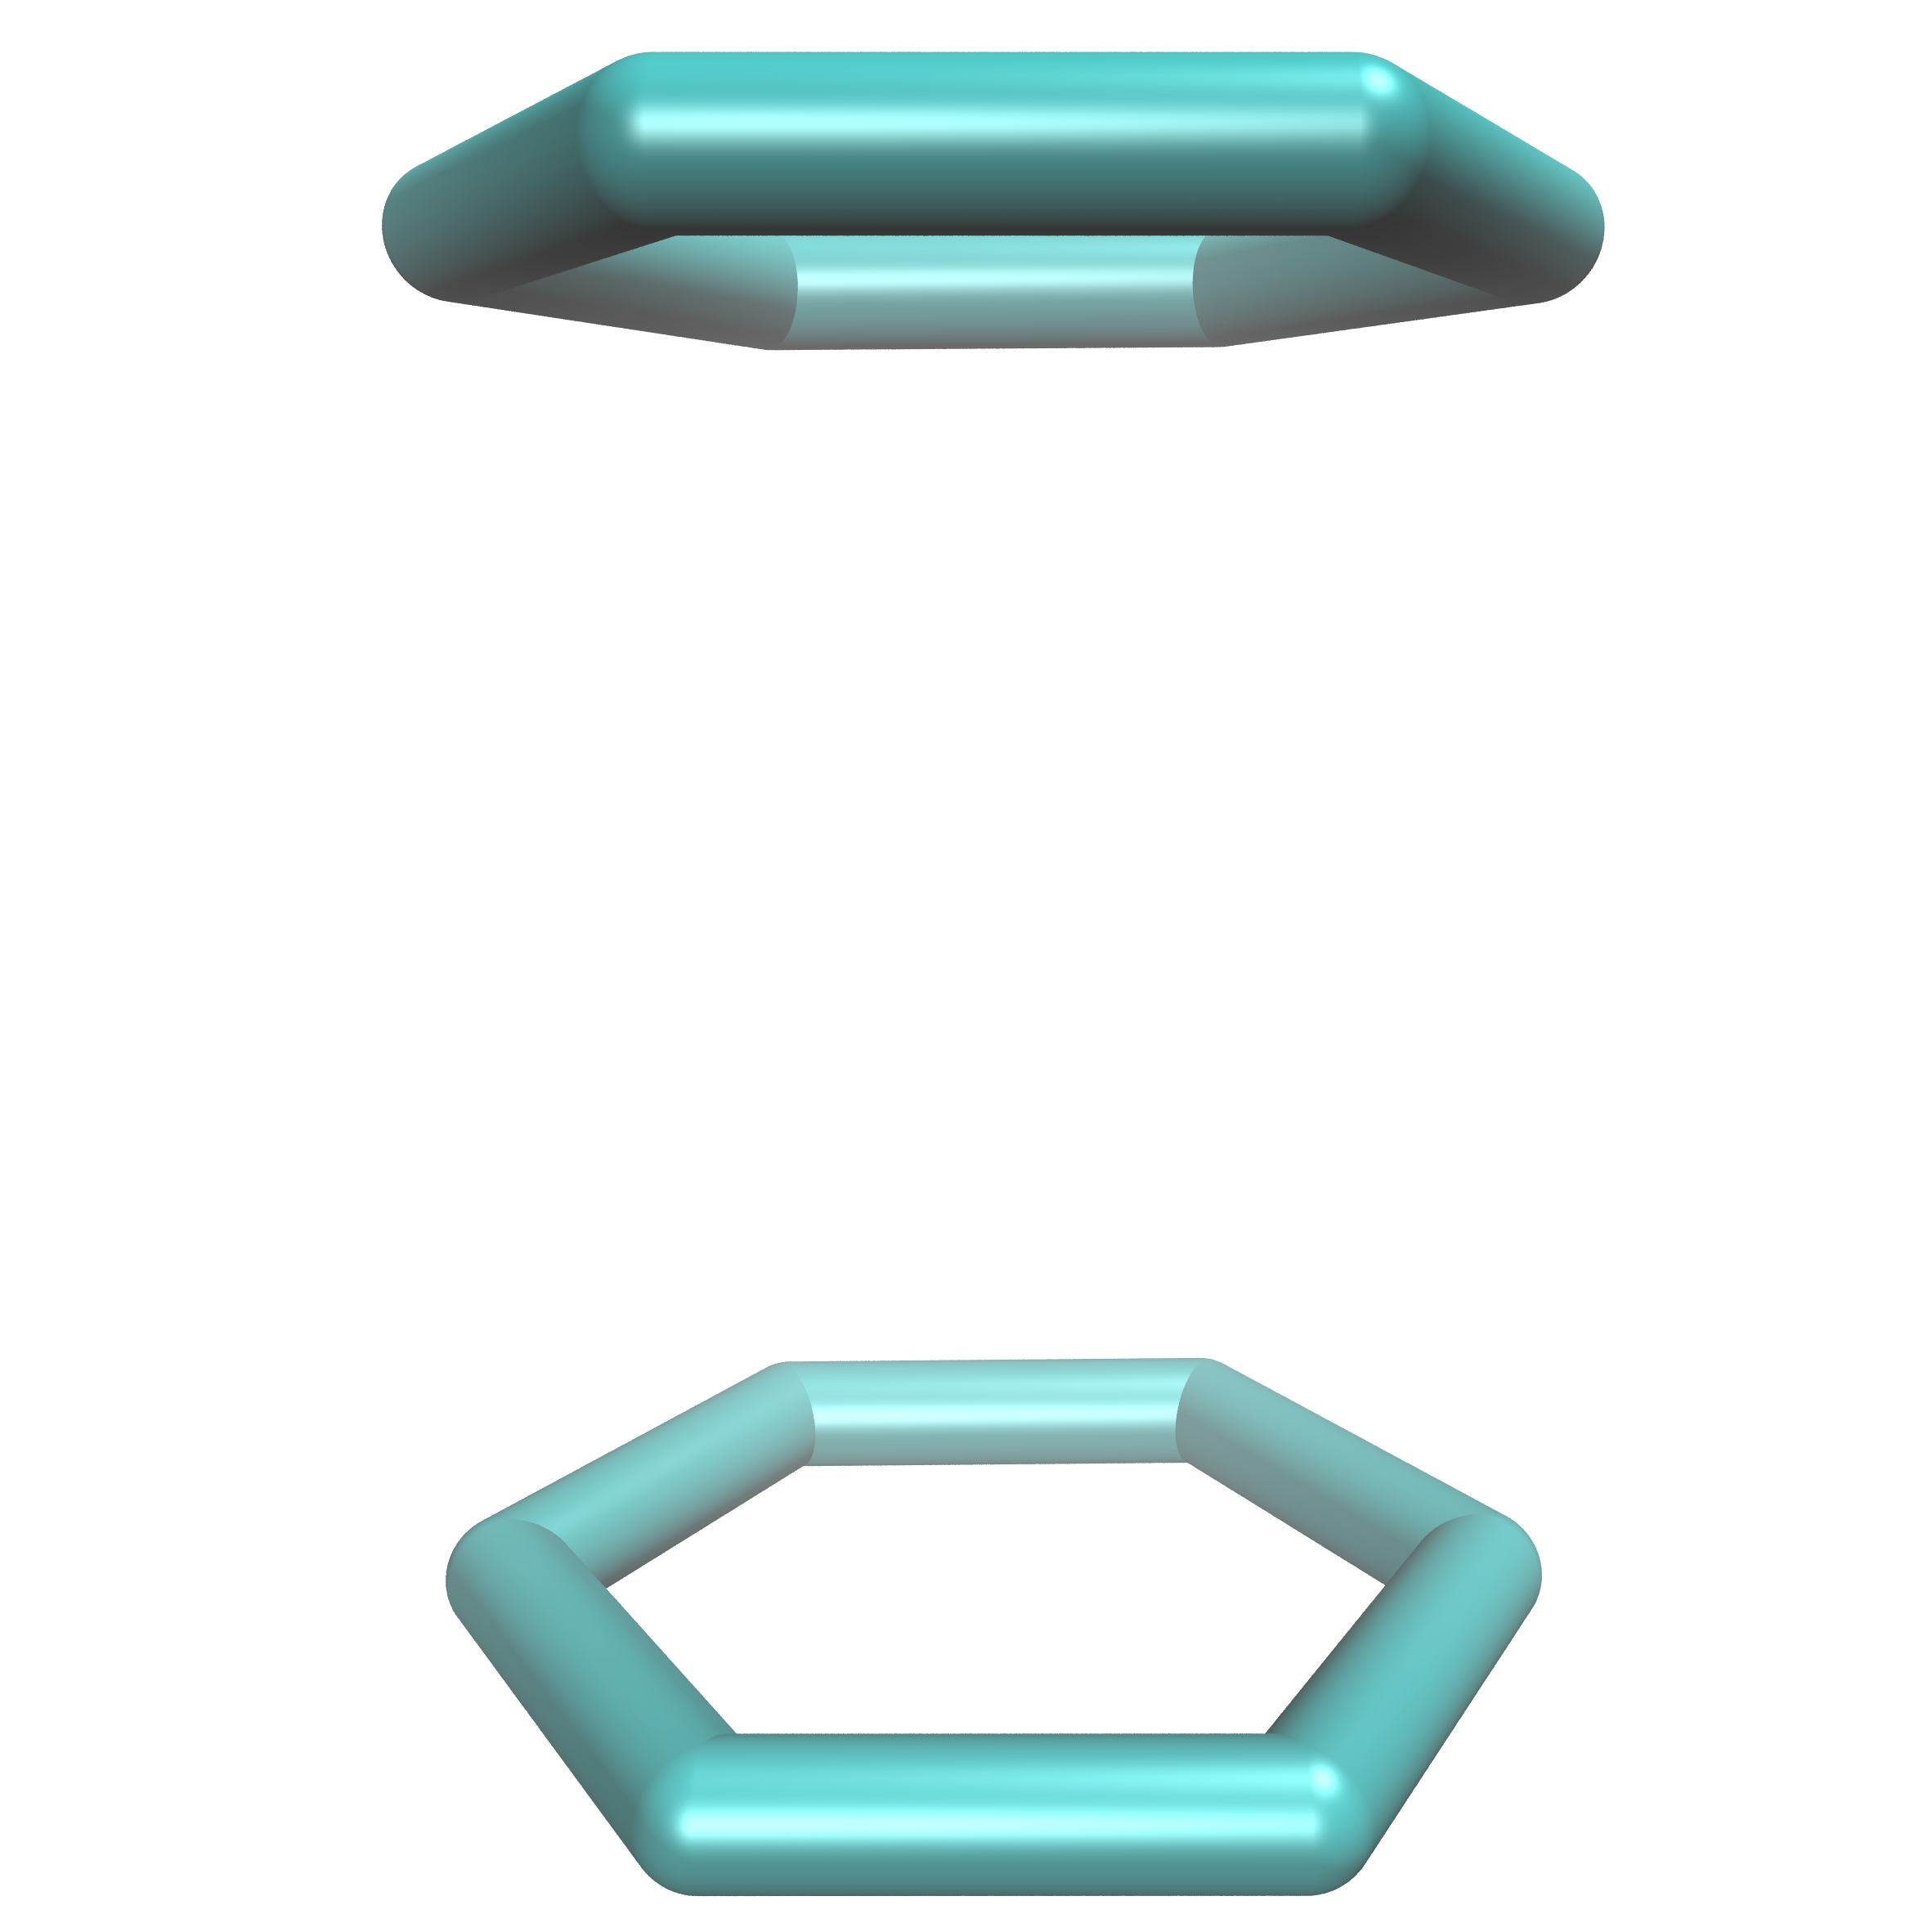
\includegraphics[width=\textwidth]{sandwiched.png}
		\caption{}\label{fig:sandwiched}
	\end{subfigure}
	\begin{subfigure}[b]{0.32\textwidth}
		\centering
		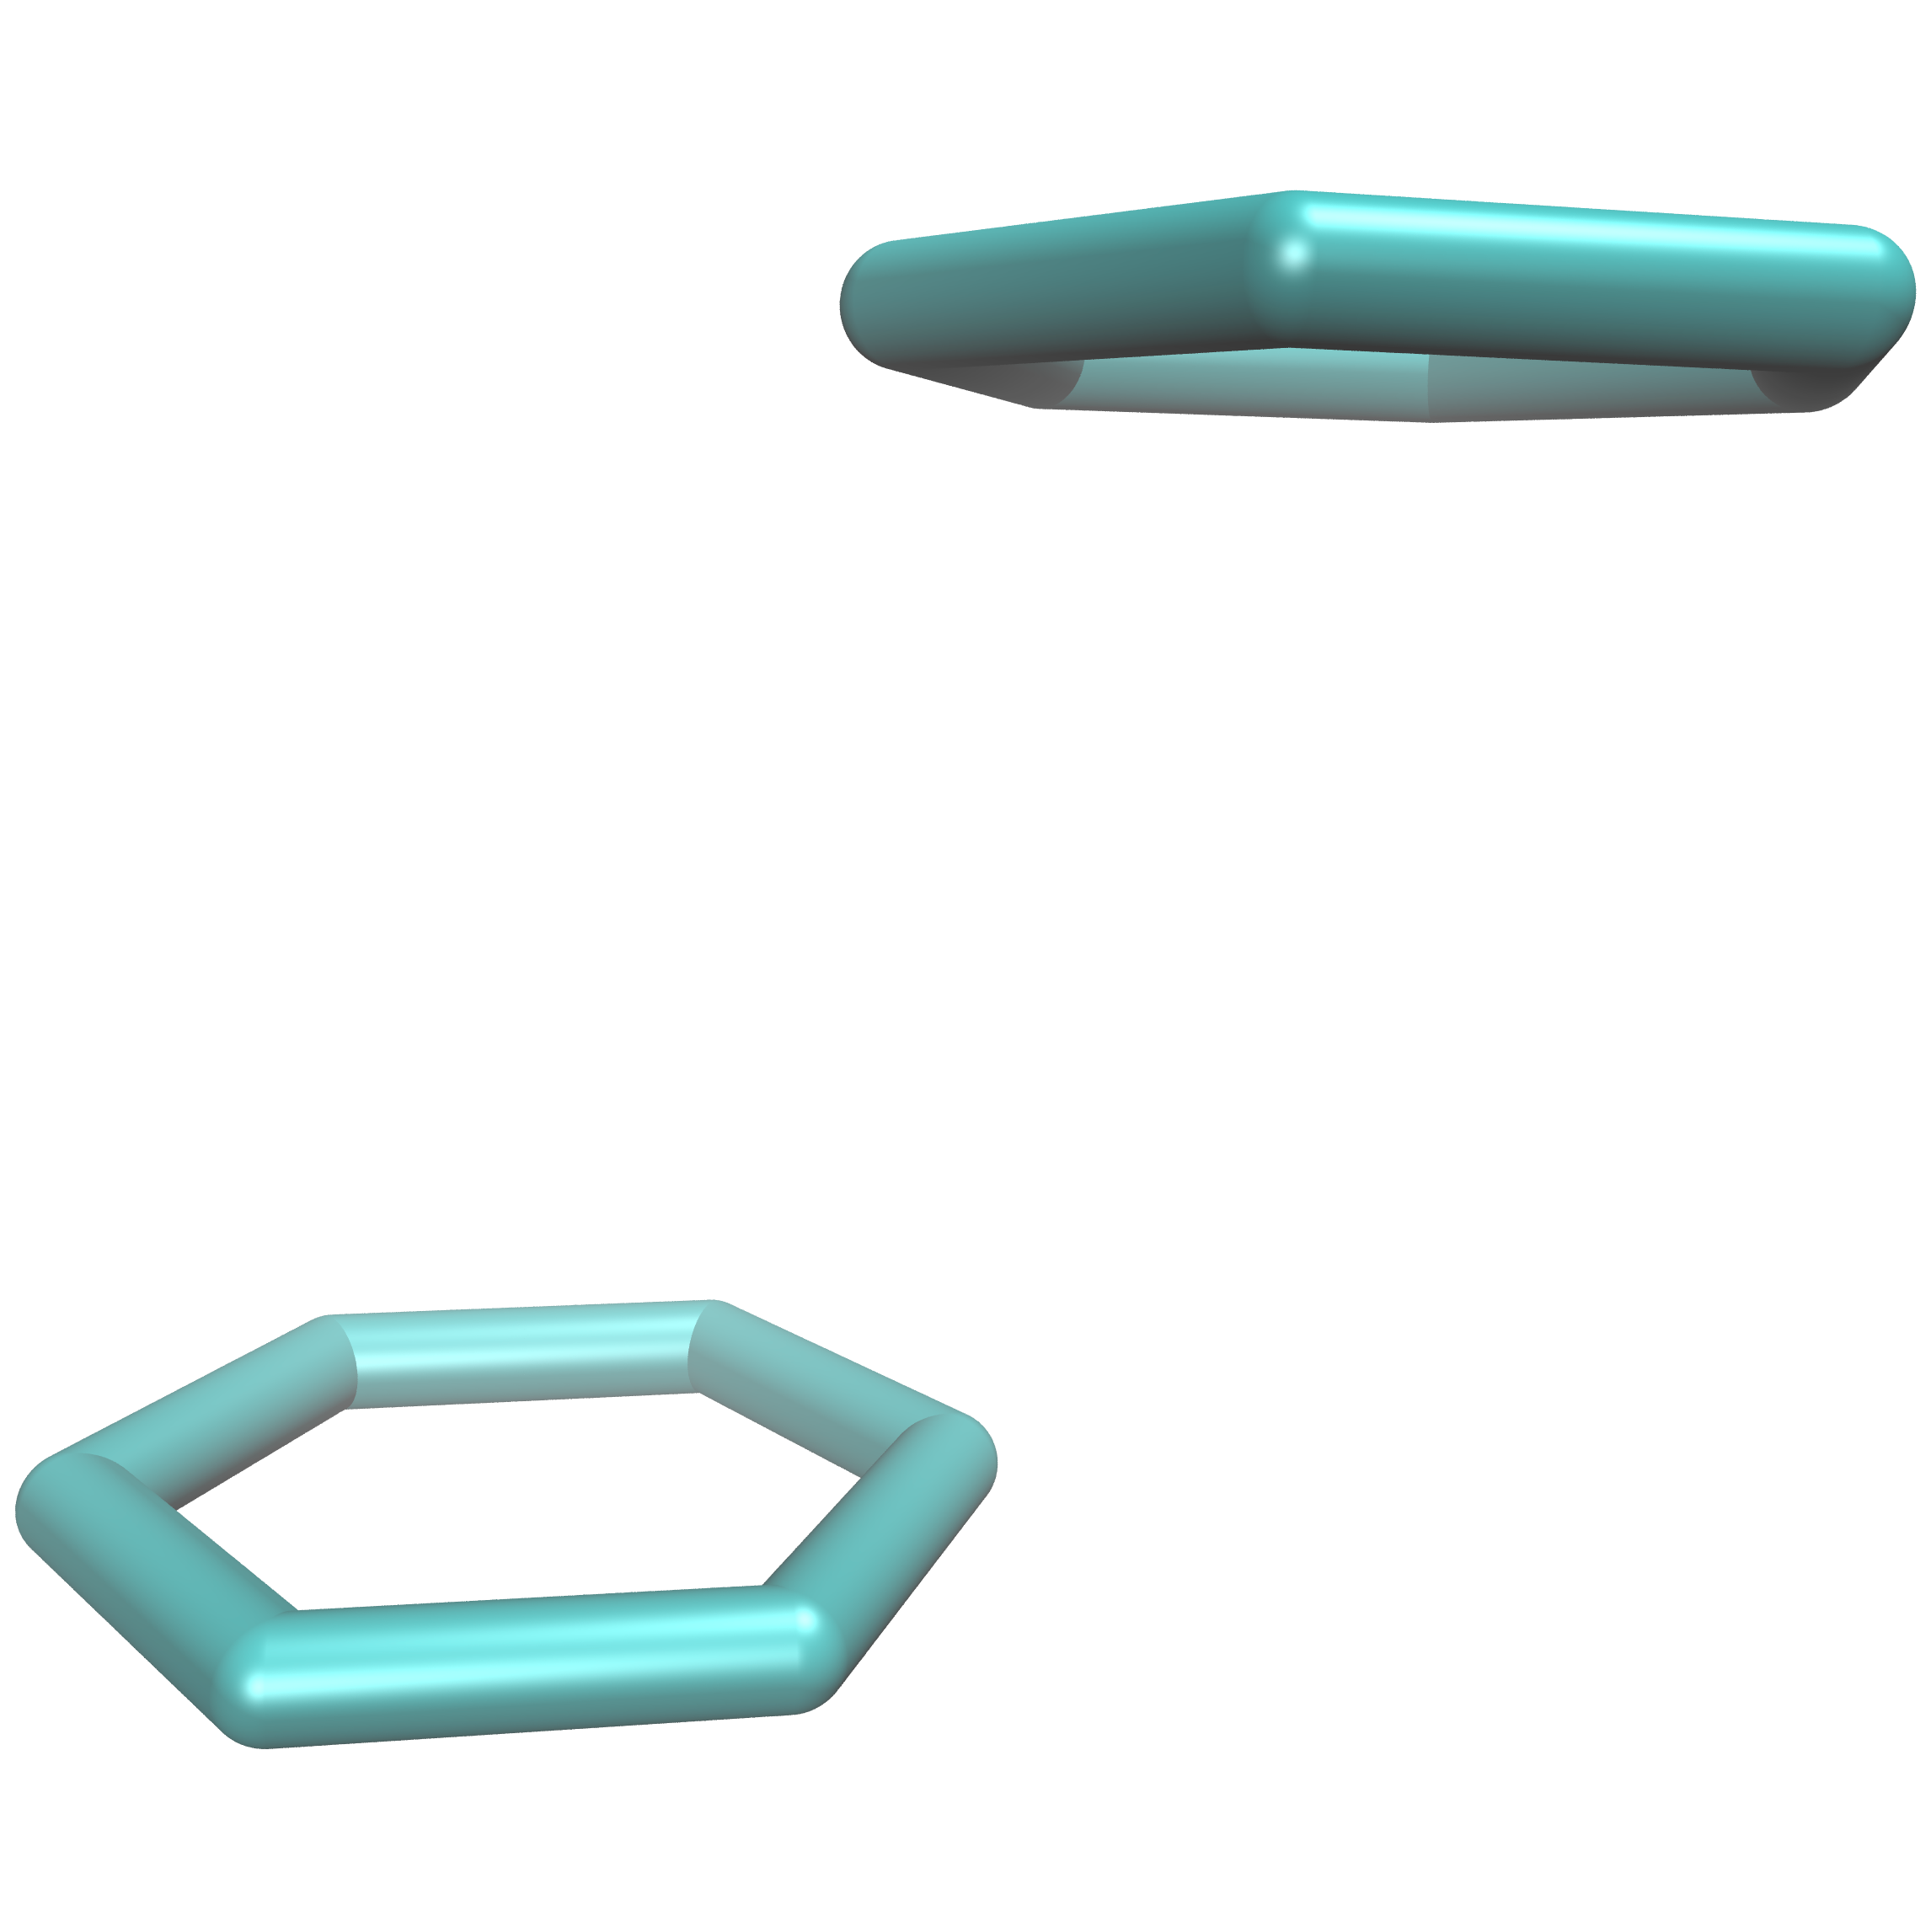
\includegraphics[width=\textwidth]{PD.png}
		\caption{}\label{fig:pd}
	\end{subfigure}
	\begin{subfigure}[b]{0.32\textwidth}
		\centering
		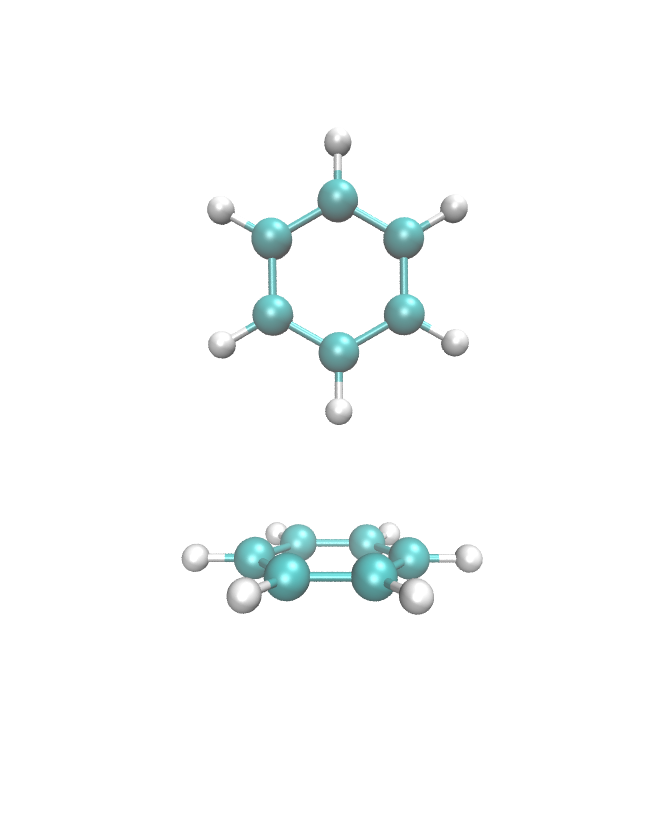
\includegraphics[width=\textwidth]{Tshaped.png}
		\caption{}\label{fig:tshaped}
	\end{subfigure}
	\vskip\baselineskip
	\begin{subfigure}[b]{0.475\textwidth}
		\centering
		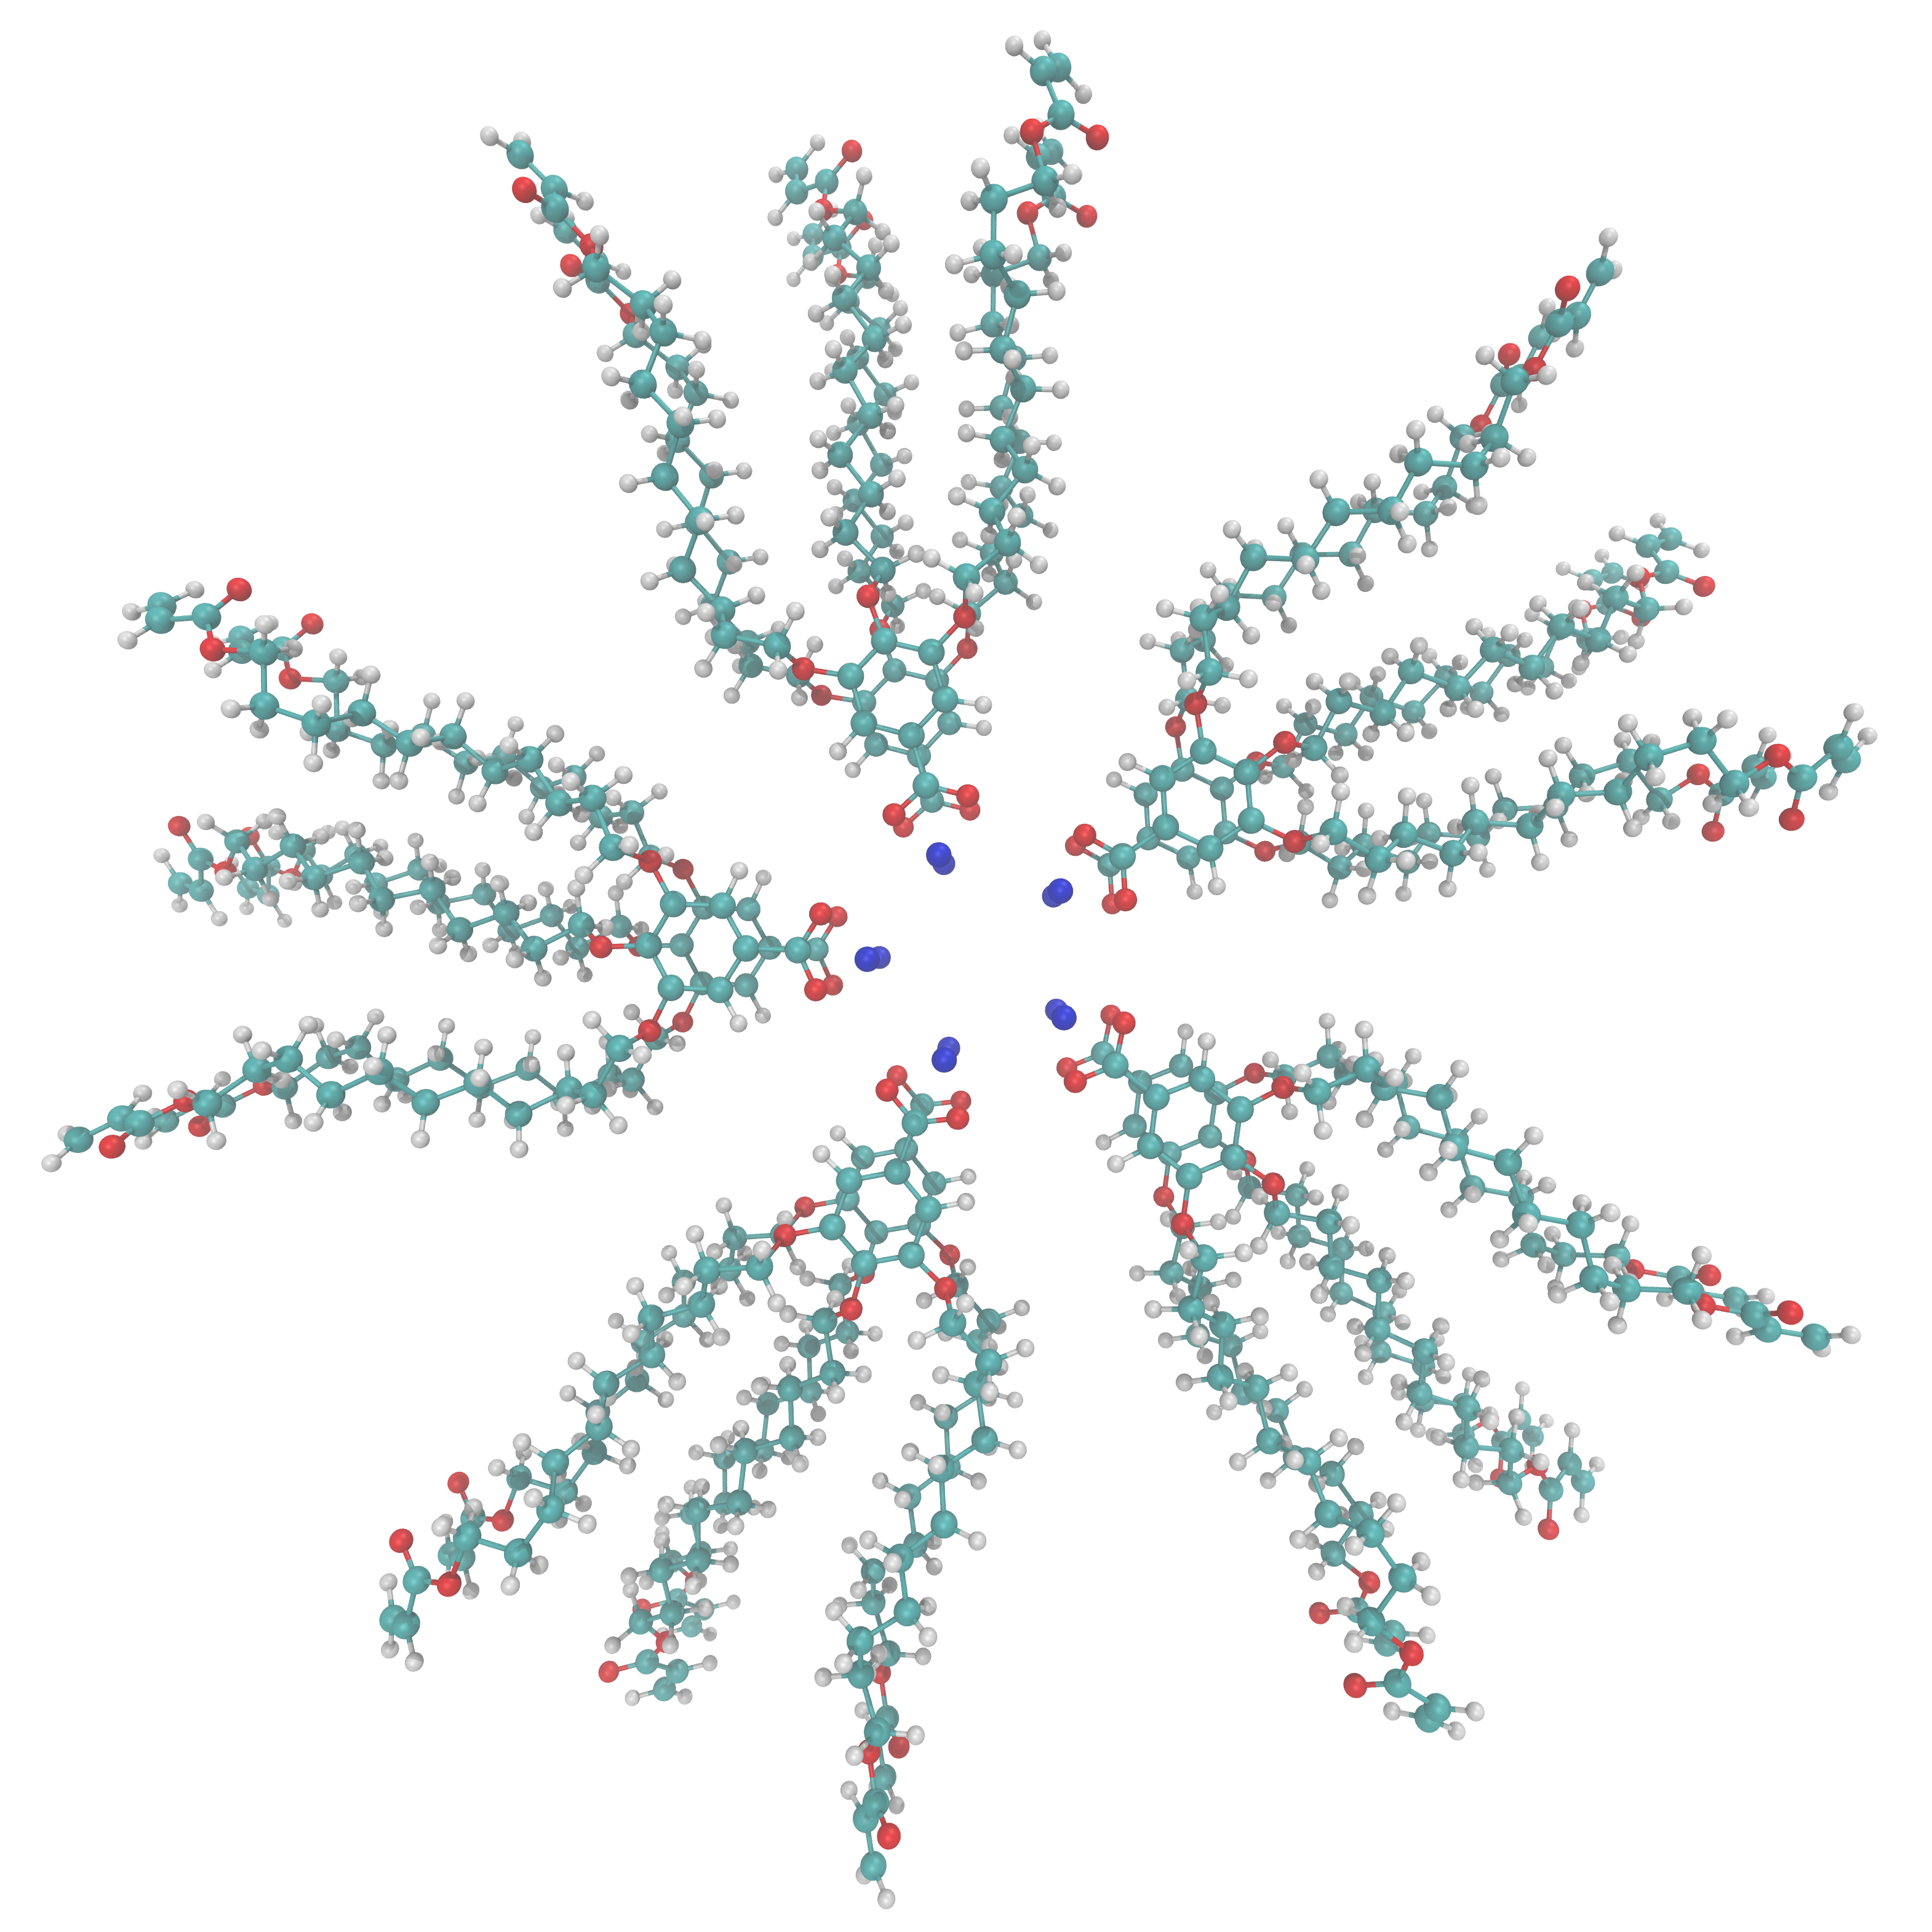
\includegraphics[width=\textwidth]{sandwichedlayers.png}
		\caption{}\label{fig:sandwichedlayers}
	\end{subfigure}
	\begin{subfigure}[b]{0.475\textwidth}
		\centering
		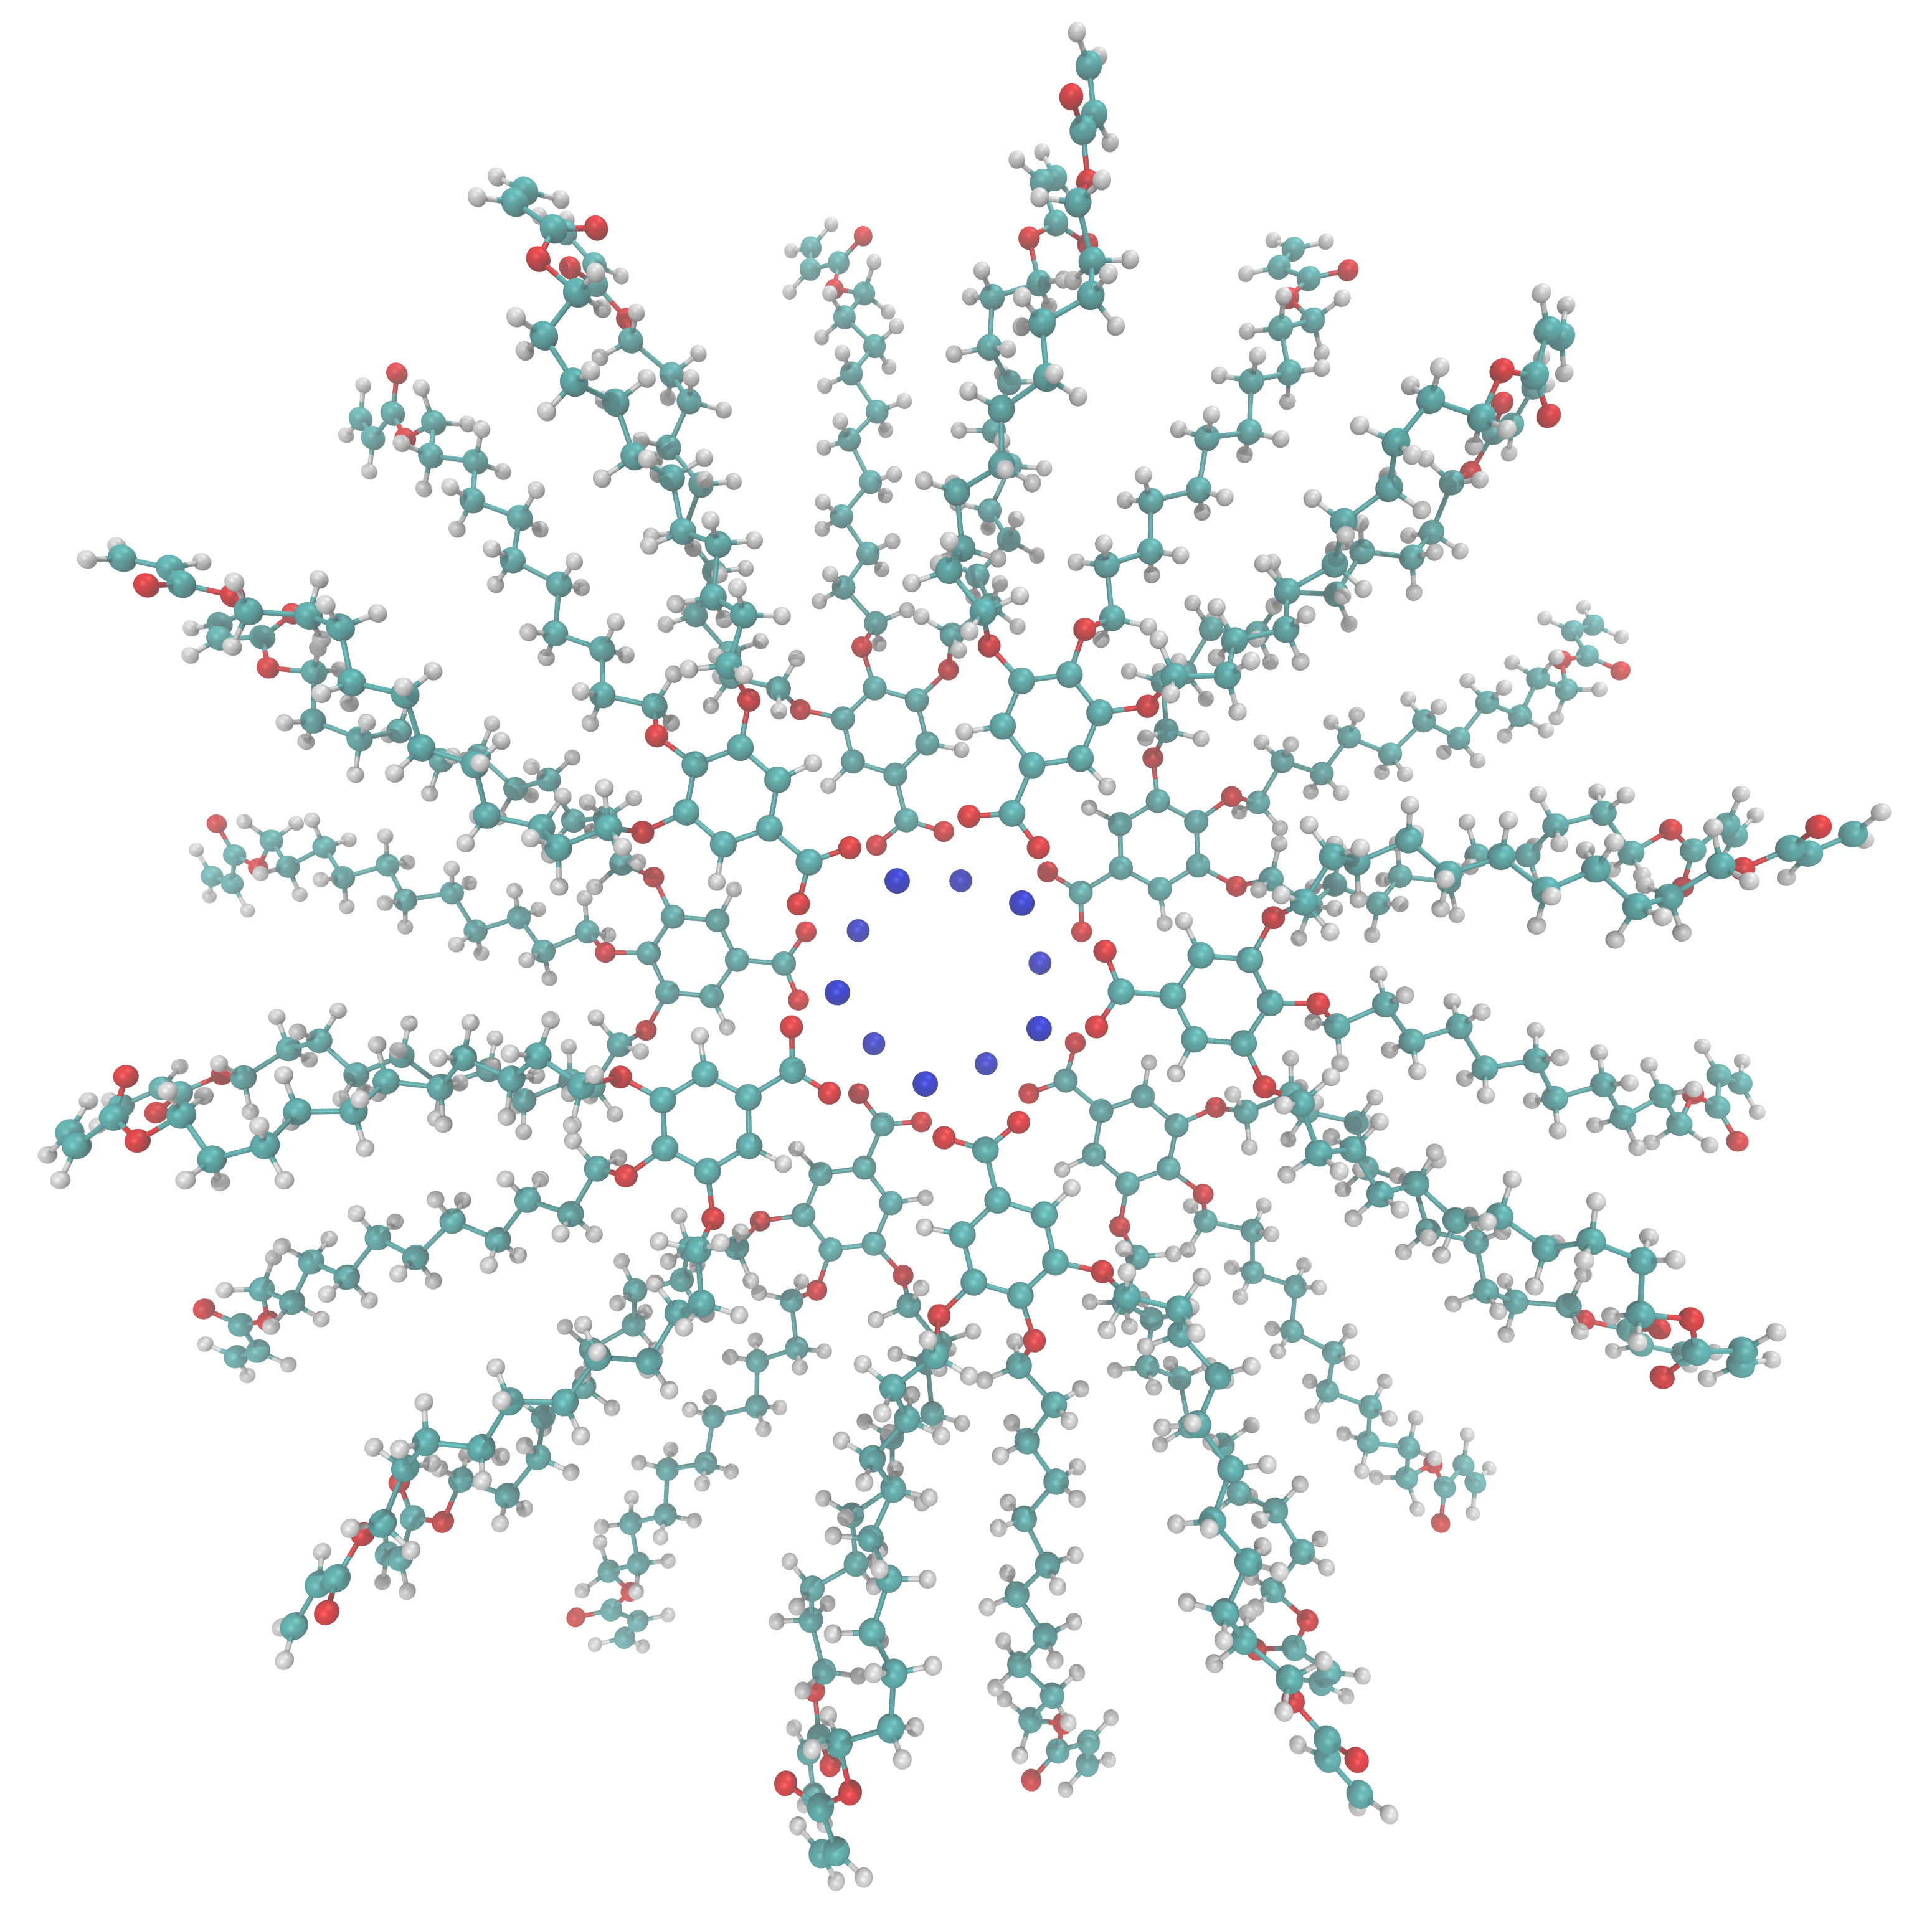
\includegraphics[width=\textwidth]{offsetlayers.png}
		\caption{}\label{fig:offsetlayers}
	\end{subfigure}
	\caption{(a) Sandwiched benzene dimers stack 3.8 \angstrom~apart. (b) Parallel-Displaced benzene dimers stack
	3.4 \angstrom~vertically and 1.6 \angstrom~horizontally apart. (c) T-shaped benzene dimers stack 5.0 \angstrom~apart. 
	(d) Two monomer layers stacked in the sandwiched configuration (e) Two monomer layers stacked in the parallel-displaced
	configuration }\label{fig:stacking}
  \end{figure}
  
  We explored the pore composition by measuring the average number densities of
  various monomer components as a function of distance from the pore centers. The
  centers of the pores were located using the same method used to calculate the
  equilibrium pore spacing. We looked at the average number density of sodium
  ions, aromatic rings and carbon atoms making up the monomer tails. The radial
  distance of all atoms in each group from the pore centers are binned, then
  normalized by the volume of the annulus defined by the bin edges and z box
  vector.
  %BJC: Maybe write an equation here? It's hard to say precisely how I did it
  %in words without it sounding confusing 

  We calculated ionic conductivity using two different methods for robustness.
  The Nernst-Einstein relation relates the DC ionic conductivity to ion
  diffusivity, $D$, concentration, $C$, ion charge, $q$, the boltzmann constant,
  $k_b$, and temperature, $T$: $$\sigma = \dfrac{q^2CD}{k_b T}$$. 
  Sodium ion diffusion coefficients were found by calculating the slope
  of the linear region of the z-direction mean square displacement curve as
  indicated by the einstein relation \cite{einstein_investigations_1956}.] We
  looked at the MSD plot to determine where to begin and end a linear fit. Ion
  concentration was measured with respect to the volume of the entire unit cell. 

  The second method, termed the 'Collective Diffusion' model, measures the
  movement of the collective variable, Q, which is defined as the amount of
  charge transfer through the system and can be thought to represent the center
  of charge of the system. The conductance, $\gamma$ of the system can be
  calculated as: $$ \gamma = \dfrac{D_Q}{k_b T} $$. Conversion to ionic
  conductivity is achieved by multiplying by channel length and dividing by the
  membrane cross sectional area.  $D_Q$ is the diffusion coefficient of the
  collective variable Q. It can be calculated using the einstein relation.  A
  full derivation of the model can be accessed elsewhere 
  \cite{liu_collective_2013}.

  \section*{Results and Discussion}
  
  \subsection*{Determination of Nanoscopic Structural Details}
  
  We will now address the questions raised in the introduction in the order
  that they were asked.  %BJC: Not a fan of this transition

  The simulations best support a model built with 5 monomers per layer based on
  the measured pore-to-pore distances. To discern the composition of the
  monomer layers, addressing (\ref{point:monomernum}), we ran simulations of
  systems created with 4 - 8 monomers per layer. Systems were built in both the
  parallel displaced and sandwiched configurations and prepared according to the
  dry equilibration procedure. All systems are stable after 400 ns of simulation.
  In a sense, all systems are at least metastable, addressing
  \ref{point:metastable}, however not all will make physical sense or fit the
  experimental profile that we are looking to match. Figure ~\ref{fig:p2p}
  shows the pore spacing for all systems tested. Systems built with 5 monomers in
  each layer equilibrate to a pore spacing that is most consistent with the
  experimental value of 4.12 nm derived from SAXS measurements
  (Figure~\ref{fig:SAXS}). The remainder of this discussion will focus on the
  analysis of systems built with 5 monomers per layer.

  We learned that layers are well-defined and persistent, answering
  (\ref{point:layers}). We verified our conclusion by plotting the pair
  correlation function, $g(z)$ calculated between atoms along the length of the
  pores (Fig~\ref{fig:zdf}). We measured $g(z)$ with respect to aromatic rings in
  the head groups and, separately, with respect to carbon atoms in the alkane
  chains. We see that sandwiched configuration layers stack 4.39 \angstrom apart
  while parallel displaced configuration layers stack 4.38 \angstrom apart.  The
  power spectrums used to calculate the reported layer spacings are given in the
  Supplemental Information.

 \begin{figure}
	\centering
	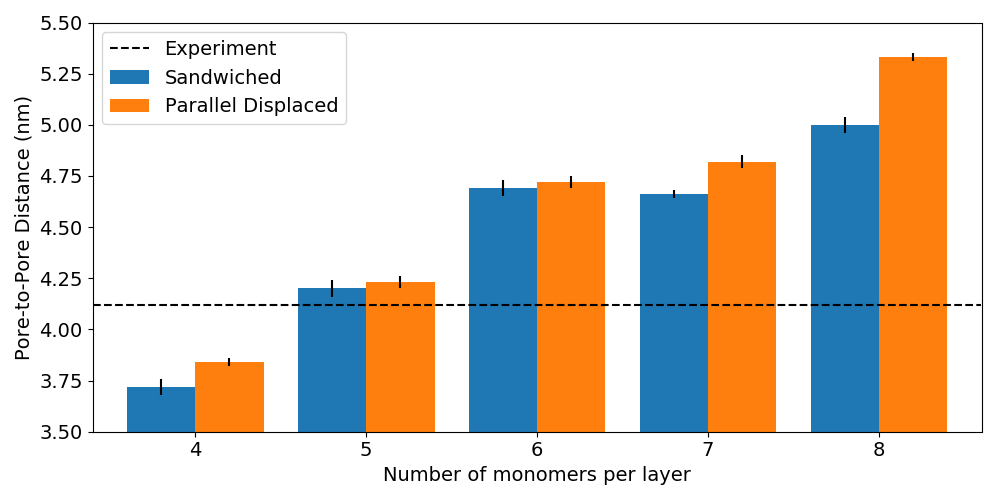
\includegraphics[width=0.5\linewidth]{p2p.png}
	\caption{The pore spacing (given in nm) of the model increases as
	number of monomers in each layer increases. The pore spacing of a system
	starting in the sandwiched configuration is systematically lower than 
	that started in an offset configuration. Systems built with 5 monomers
	per layer in a parallel displaced configuration result in a pore spacing
	closest to the experimental 4.12 nm}~\label{fig:p2p}
  \end{figure}  

  \begin{figure}
        \centering
        \begin{subfigure}{0.45\textwidth}
                \centering
                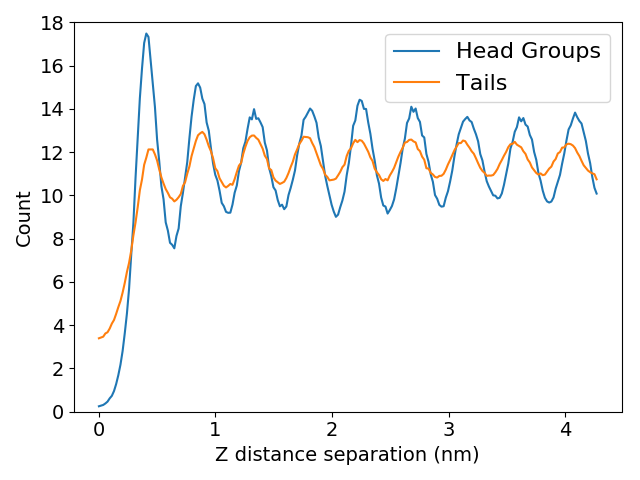
\includegraphics[width=\textwidth]{zdf_overlay_layered.png}
                \caption{}\label{fig:zdf_layered}
        \end{subfigure}
        \begin{subfigure}{0.45\textwidth}
                \centering
                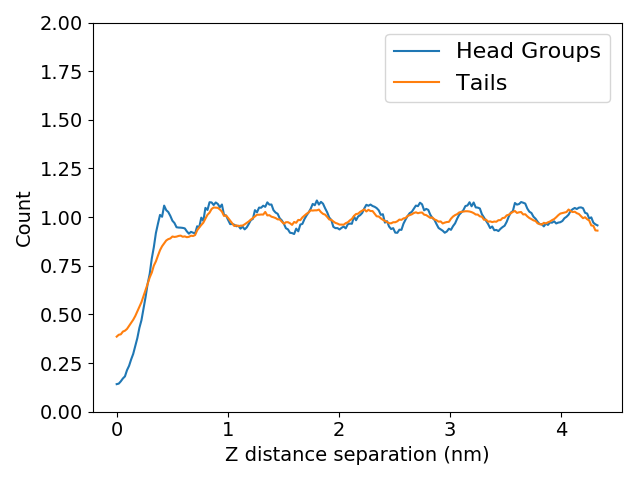
\includegraphics[width=\textwidth]{zdf_overlay_offset.png}
                \caption{}\label{fig:zdf_offset}
        \end{subfigure}
        \caption{Pair distribution functions of aromatic carbons for the
        (a) 5 monomer per layer, sandwiched and (b) 5 monomer per layer,
        parallel displaced configurations. Clear periodic maxima in the
        $z$ probability density indicate distinct layers. The magnitude
        of the spikes with respect to the average suggest that the 5
        monomer per layer, sandwiched configuration possesses a higher
        degree of layer partitioning.}\label{fig:zdf}
  \end{figure}

  We answer question (\ref{point:orientation}) by simulating X-ray diffraction
  patterns produced from equilibrated MD trajectories. We tested systems built
  with 5 monomers per layer in the parallel displaced and sandwiched
  configurations.  Simulated patterns were generated using portions of simulation
  trajectory after equilibration. The patterns for both structures are shown and
  compared to experiment in Figure ~\ref{fig:XRDsim}.

  Simulated XRD of the sandwiched configuration contains all experimental
  features except for R-helix. R-alkanes, R-spots and R-pores appear in the
  expected locations. R-$\pi$ is also present, however it intersects R-alkanes at
  a q value lower than experiment meaning the rings prefer to stack further
  apart. 

  The parallel displaced configuration results in a simulated XRD pattern with
  the closest match to experiment. It produces the only pattern that exhibits
  all major reflections. R-alkanes, R-pores and R-$\pi$ appear as they do in the
  sandwiched configuration. R-spots appears, however with a lower intensity
  relative to R-alkanes when compared to the sandwiched configuration. R-helix
  appears apparently due to the parallel displaced aromatic rings

  \begin{figure}
  \begin{subfigure}{0.3\linewidth}
        \centering
        \vspace{-0.2em}
        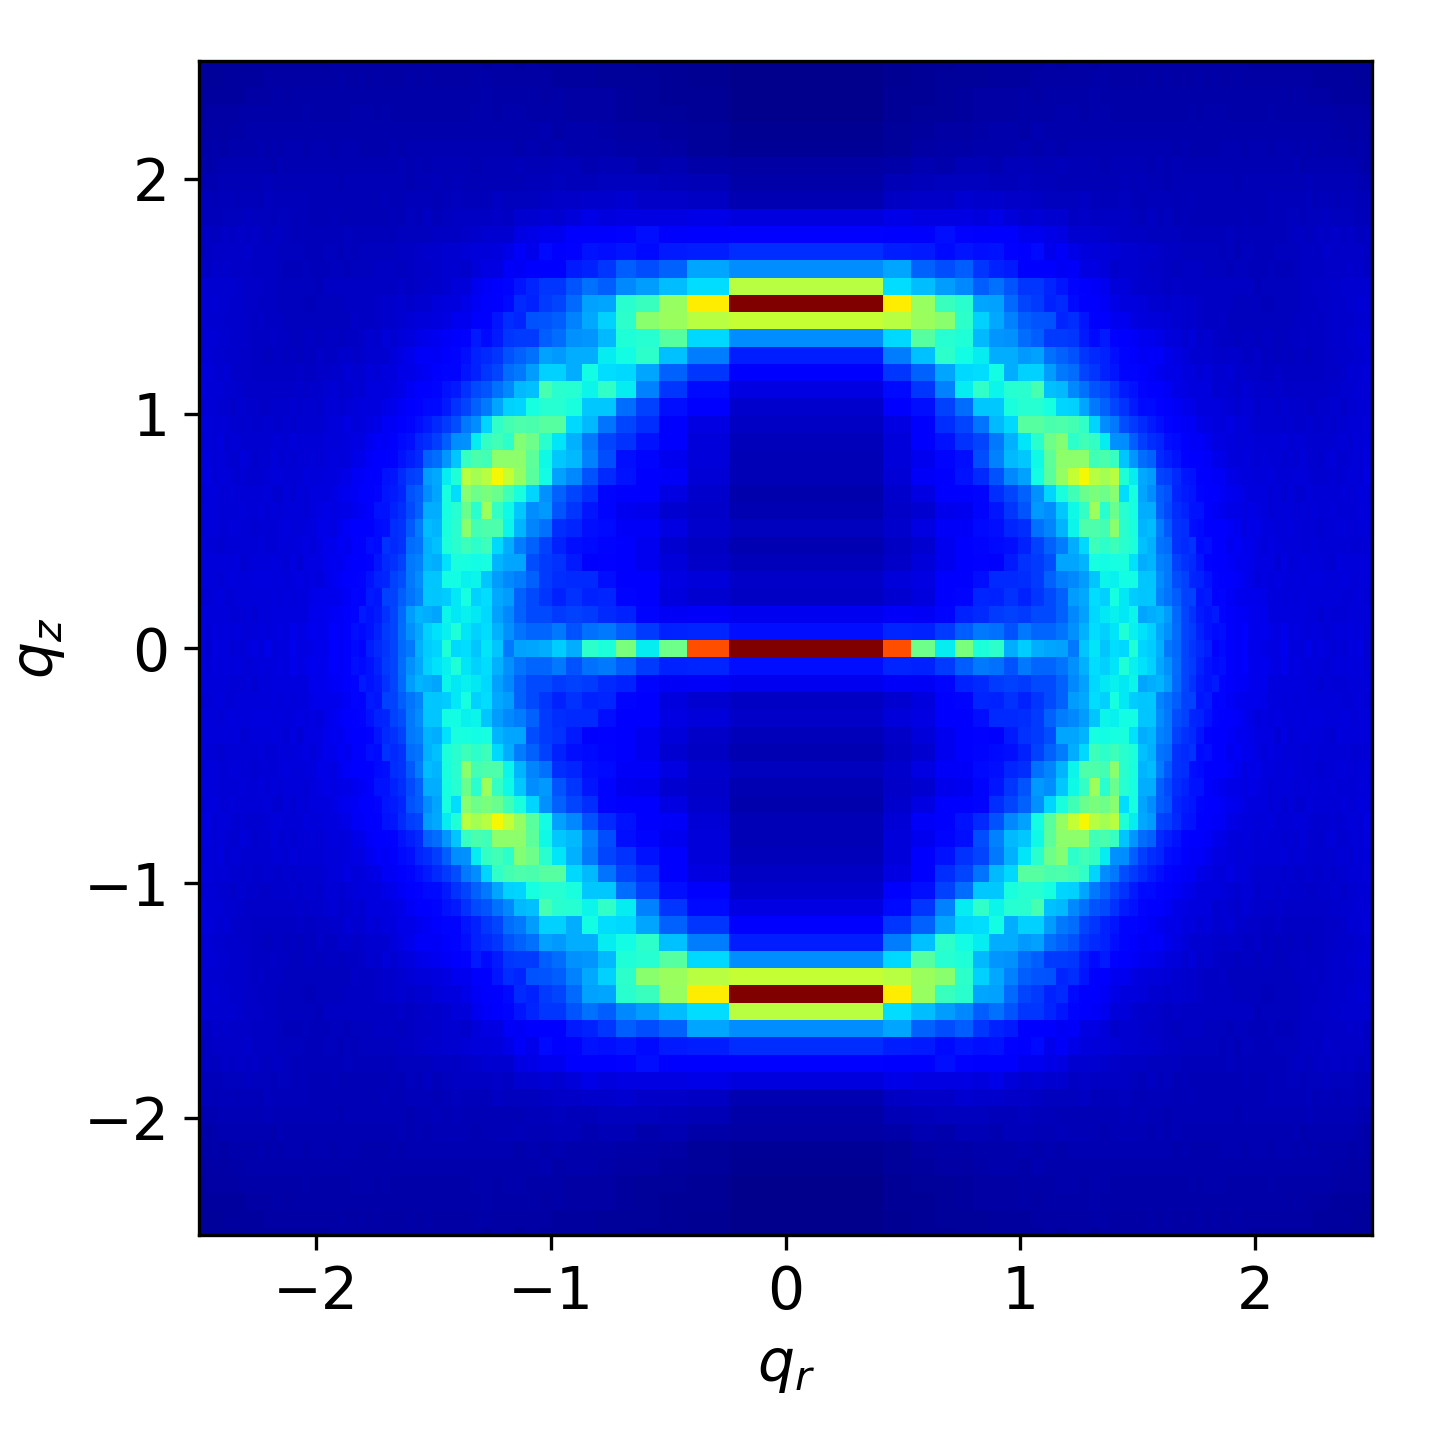
\includegraphics[width=1.018\linewidth]{layered_rzplot.png}
        \caption{}~\label{fig:rz_layered}
  \end{subfigure}
  \begin{subfigure}{0.3\linewidth}
        \centering
        \vspace{0.25em}
        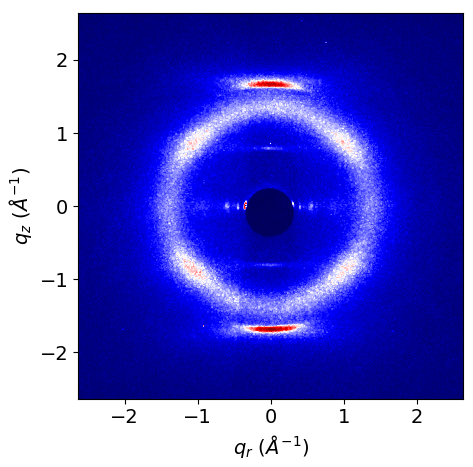
\includegraphics[scale=0.0987]{WAXS_raw.png}
        \caption{}~\label{fig:raw_waxs}
  \end{subfigure}
  \begin{subfigure}{0.3\linewidth}
        \centering
        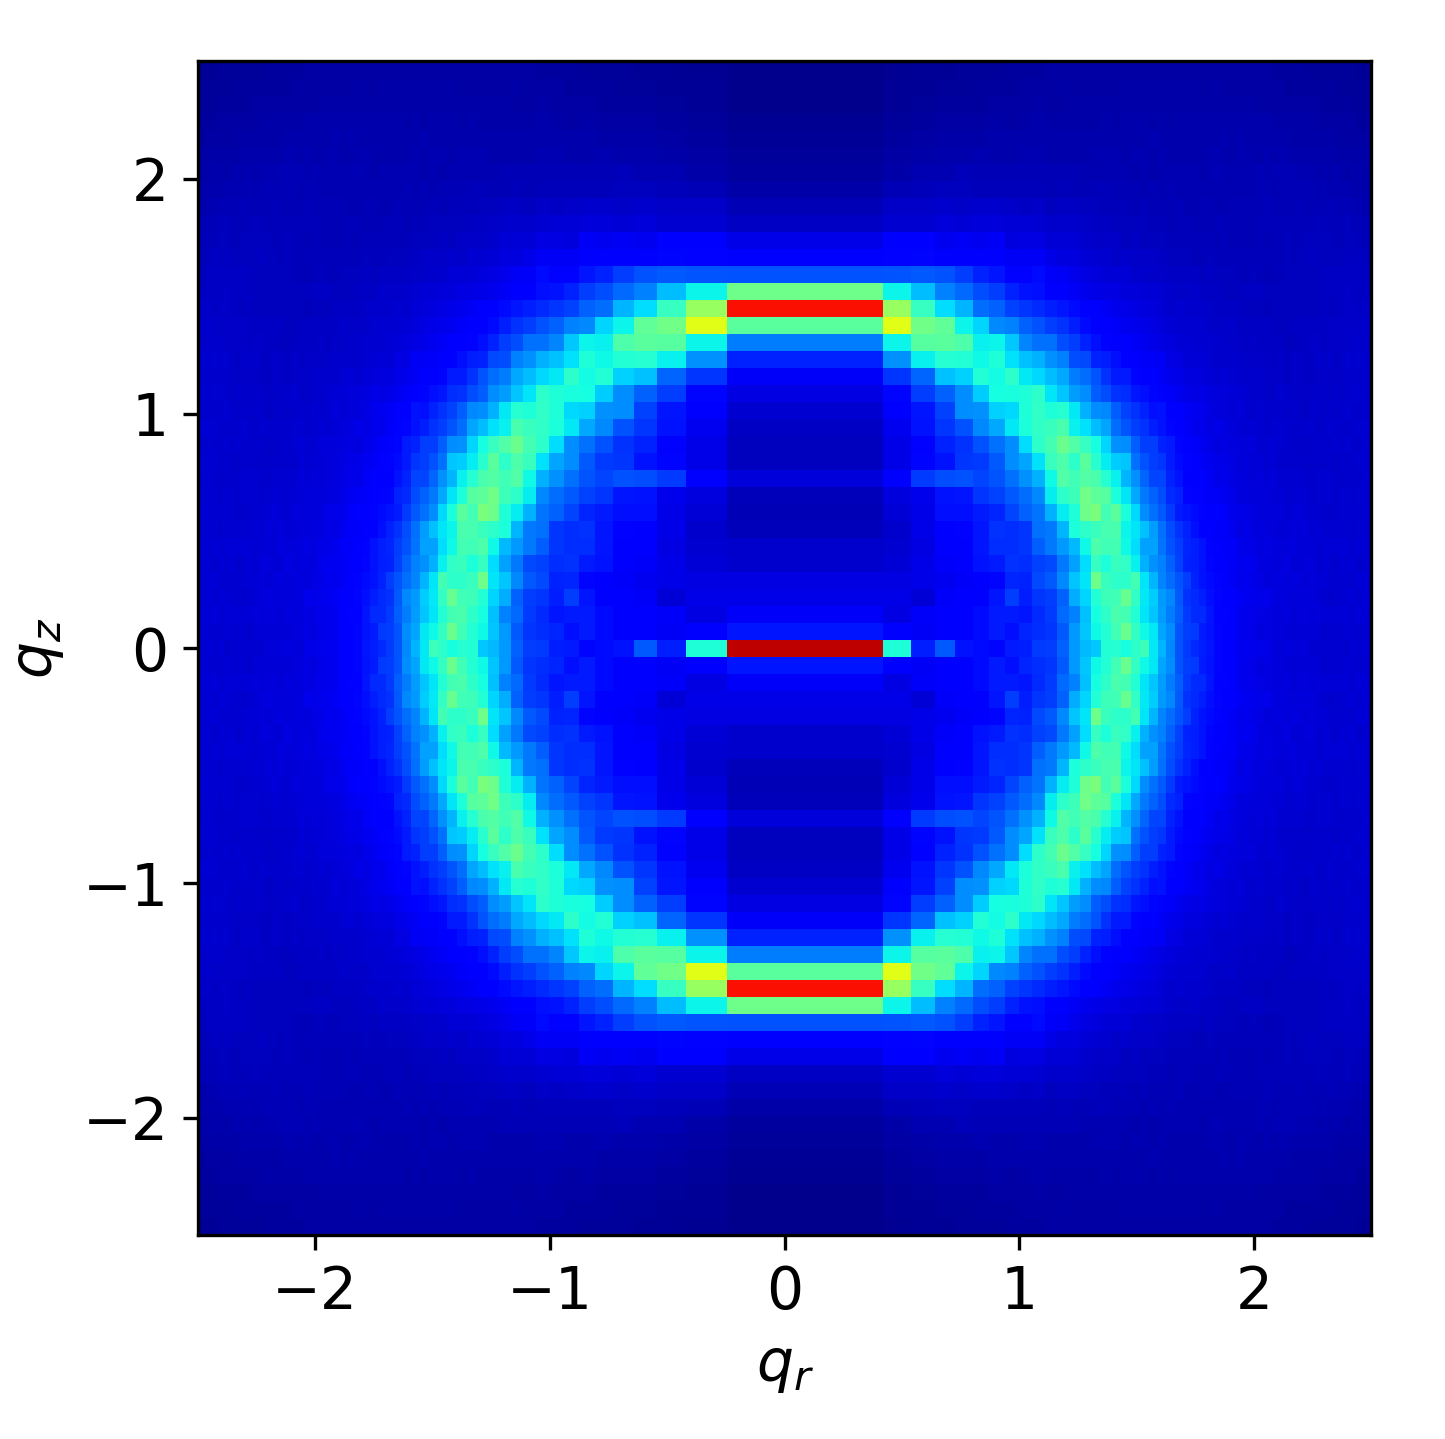
\includegraphics[width=\linewidth]{offset_rzplot.png}
        \caption{}~\label{fig:rz_offset}
  \end{subfigure}
  \begin{subfigure}{0.0544\linewidth}
        \centering
        \vspace{-3.30em}
        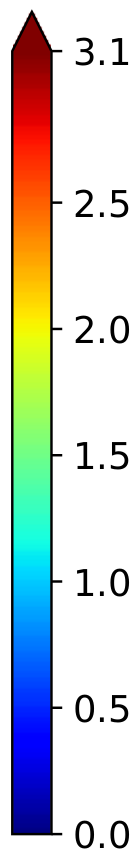
\includegraphics[width=\linewidth]{colorbar_jet.png}
  \end{subfigure}
  \caption{The simulated X-ray diffraction patterns for simulations run in the
  sandwiched (a) and parallel-displaced (c) configurations are compared to experiment (b). 
  The parallel displaced configuration is the only one that exhibits all major
  reflections of interest to some degree}
  \end{figure}

  R-spots, which appears in both simulated XRD patterns, is a result of
  hexagonal alkane chain packing. Previously, the spots in the diffraction
  pattern had been explained as the product of tilted alkane chains. We measured
  the tilt angle of the alkane chains and showed that our system equilibrates to
  an average tilt angle close to zero degrees ~\ref{fig:tilt}. To understand the
  origin of the spots, we determined which atoms gave rise to the feature. Since
  R-spots is present as higher intensity spots within R-alkanes, it is likely
  that the spots arise as a consequence of the tails. By removing atoms from the
  trajectory and simulating a diffraction pattern, we were able to isolate the
  cause of the spots to the tails (Figure~\ref{fig:tails}).  Since the tails stay
  nearly flat, we plotted the centroids of the tails and measured the angle
  between each centroid and its nearest neighbors with respect to the plane of
  the membrane (Figure~\ref{fig:centroids}).  %BJC: at one point Matt mention
  doing a correlation function instead of just measuring the angles We see
  distinct peaks in the distribution of these angles 
  (Figure~\ref{fig:tail_packing}).

  \begin{figure}
  \centering
  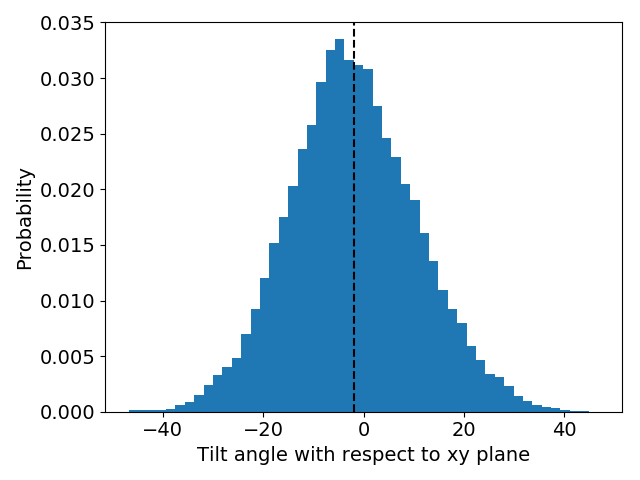
\includegraphics[width=0.5\linewidth]{tilt_dist.png}
  \caption{The tilt angle distribution of alkane chain tails with respect to the membrane plane
  indicates an average tilt angle near 7\degree which is far from the 37\degree tilt angle 
  previously used to explain R-spots}~\label{fig:tilt}
  \end{figure}

  The peaks in the tilt angle distribution are consistent with the location of
  R-spots. The peaks of interest in Figures \ref{fig:offset_tails} and
  \ref{fig:layered_tails} are located at $\pm$ 33 $\degree$ which is the same
  location where the highest intensity of spots are located on the simulated
  patterns. We confirmed this conclusion by radially integrating the 2D WAXS
  pattern for q values between 1.57 and 1.4 (real space between 4 and 4.5 \AA). We
  observe that distinct peaks appear ca. 30 $\degree$, in close agreement with
  the previously measured angle distribution
  (~\ref{fig:offset_integration}~\ref{fig:layered_integration}). We performed the
  same integration on the raw experimental data and found the angle at which
  R-spots reaches its highest intensity to be $\pm$ 37 $\degree$ which is a
  reconcilable difference with our simulated results.  

  \begin{figure}
	\centering
	\begin{subfigure}{0.45\linewidth}
		\centering
		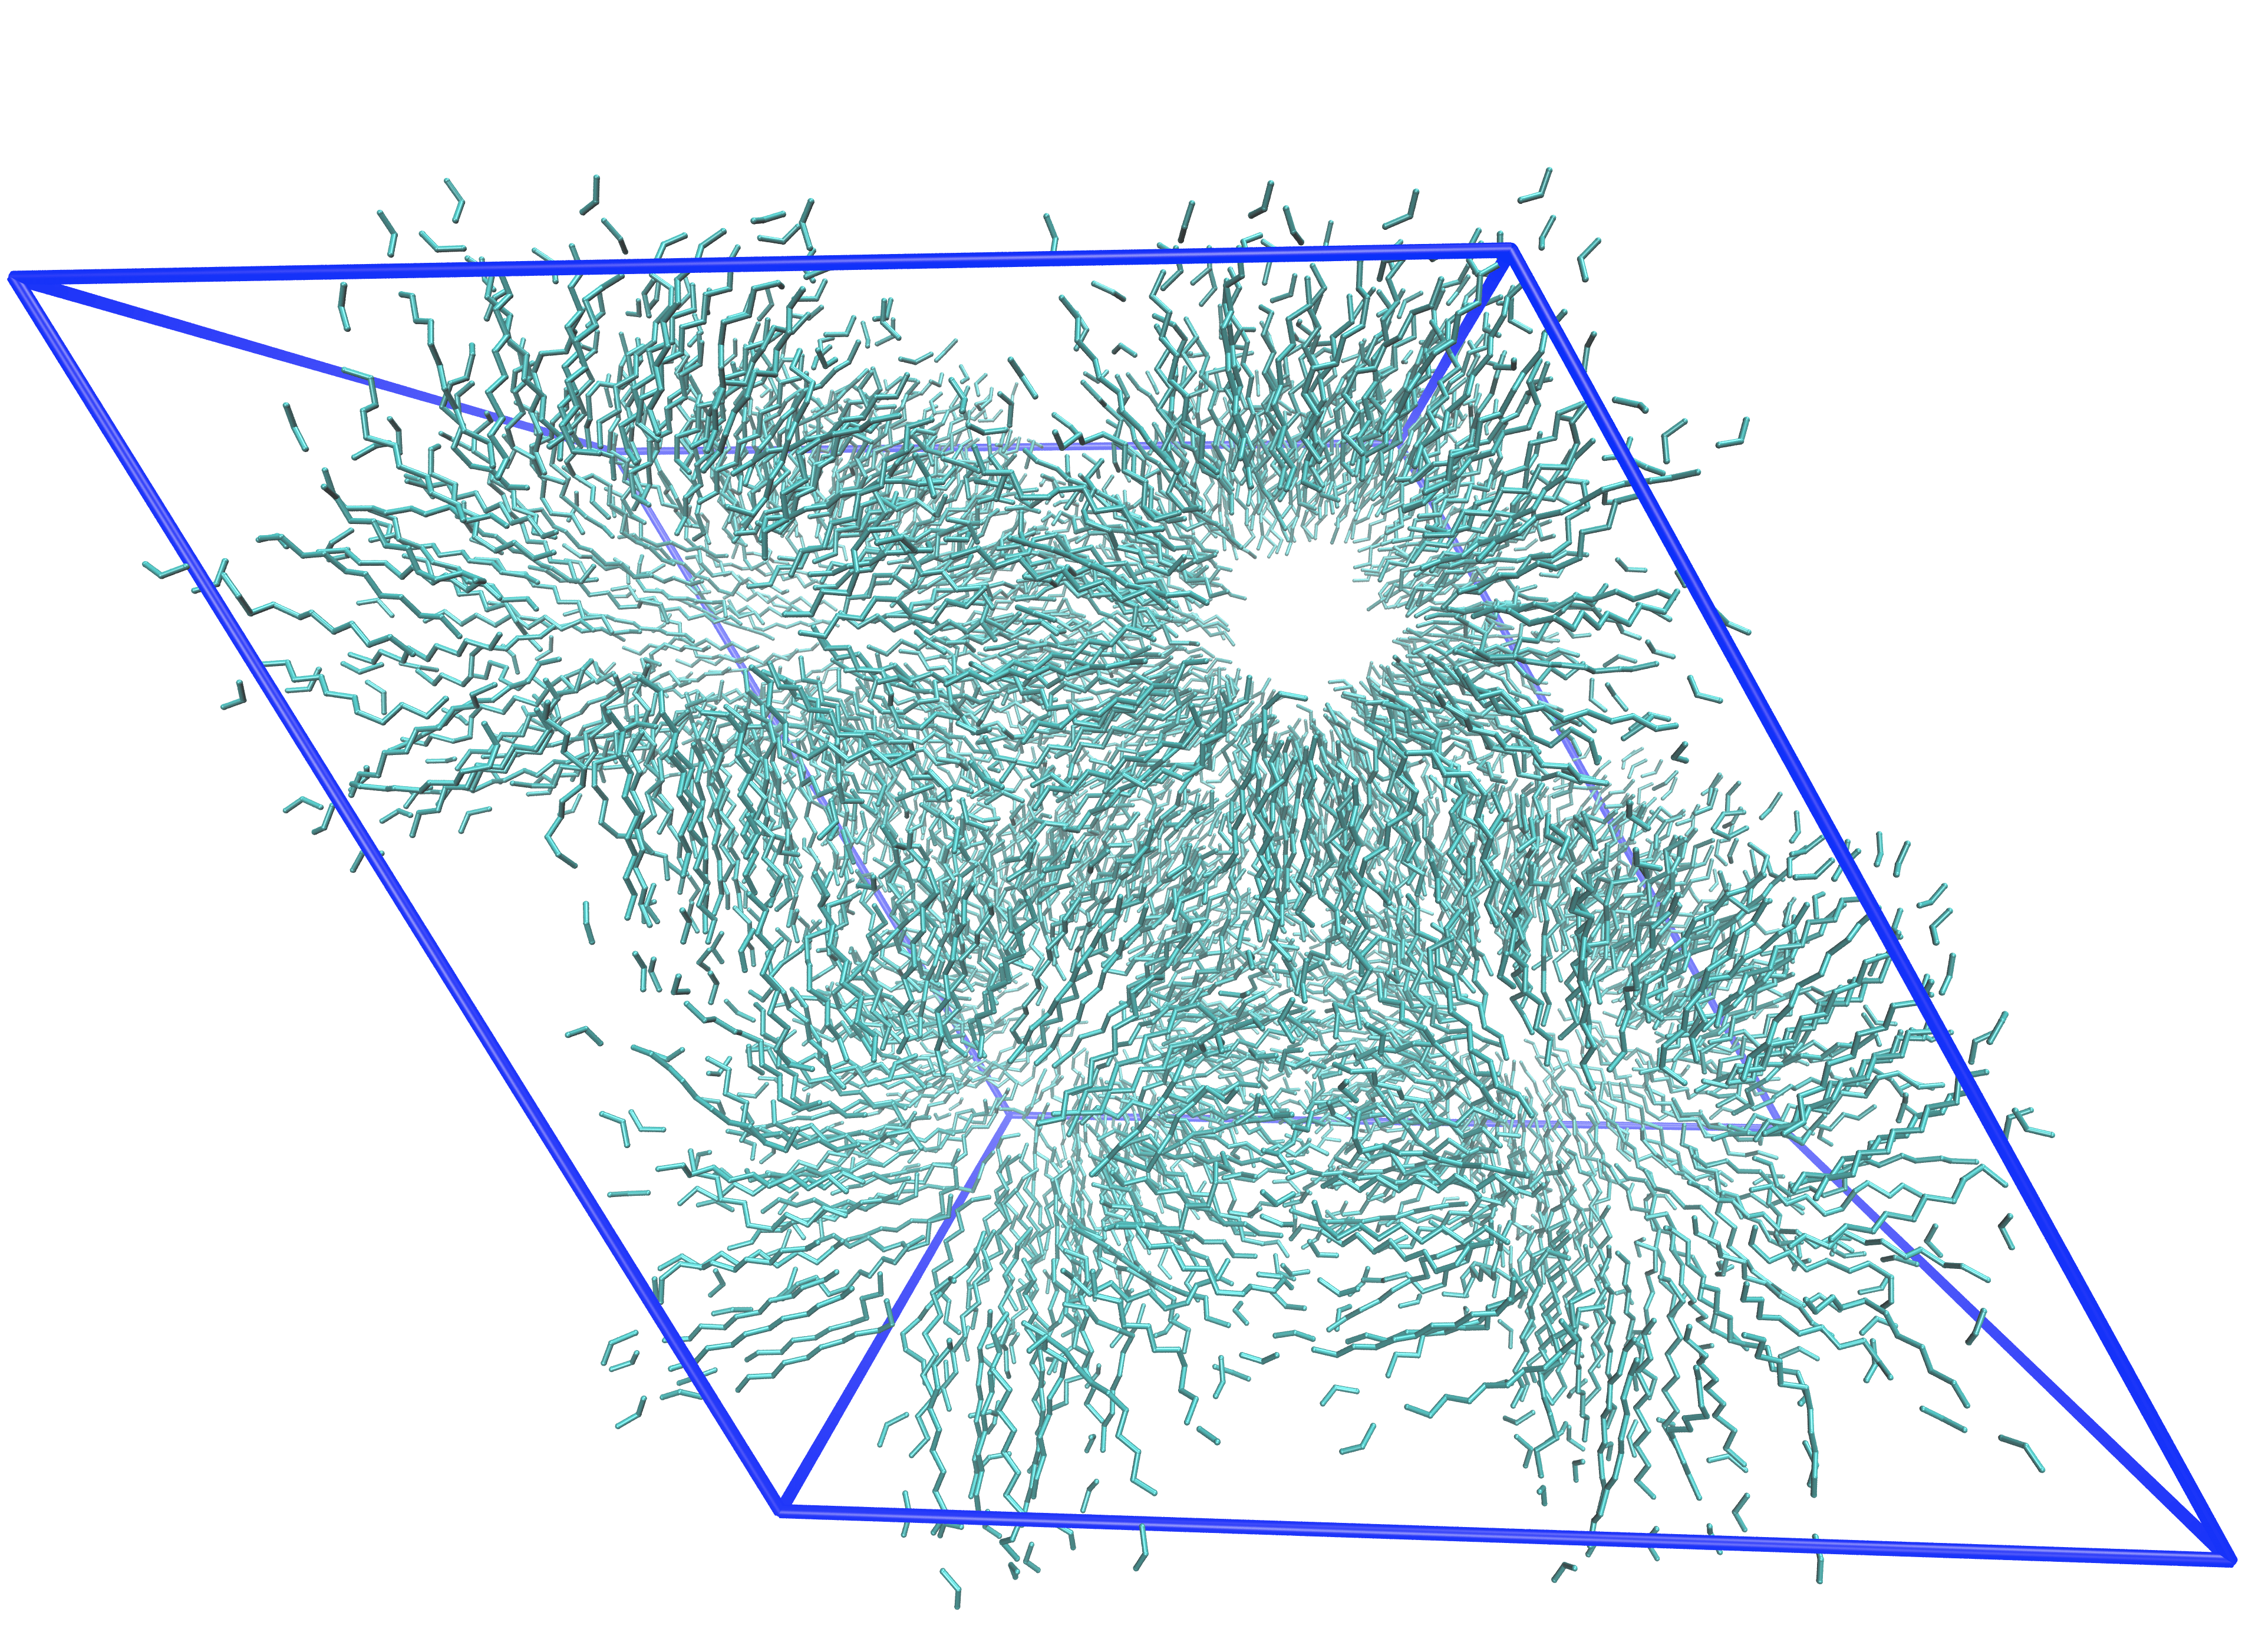
\includegraphics[width=\textwidth]{tails_topview.png}  % picture of top of unit cell with only tail atoms shown
		\caption{}\label{fig:topdown_tails_only}
	\end{subfigure}
	\begin{subfigure}{0.45\linewidth}
		\centering
		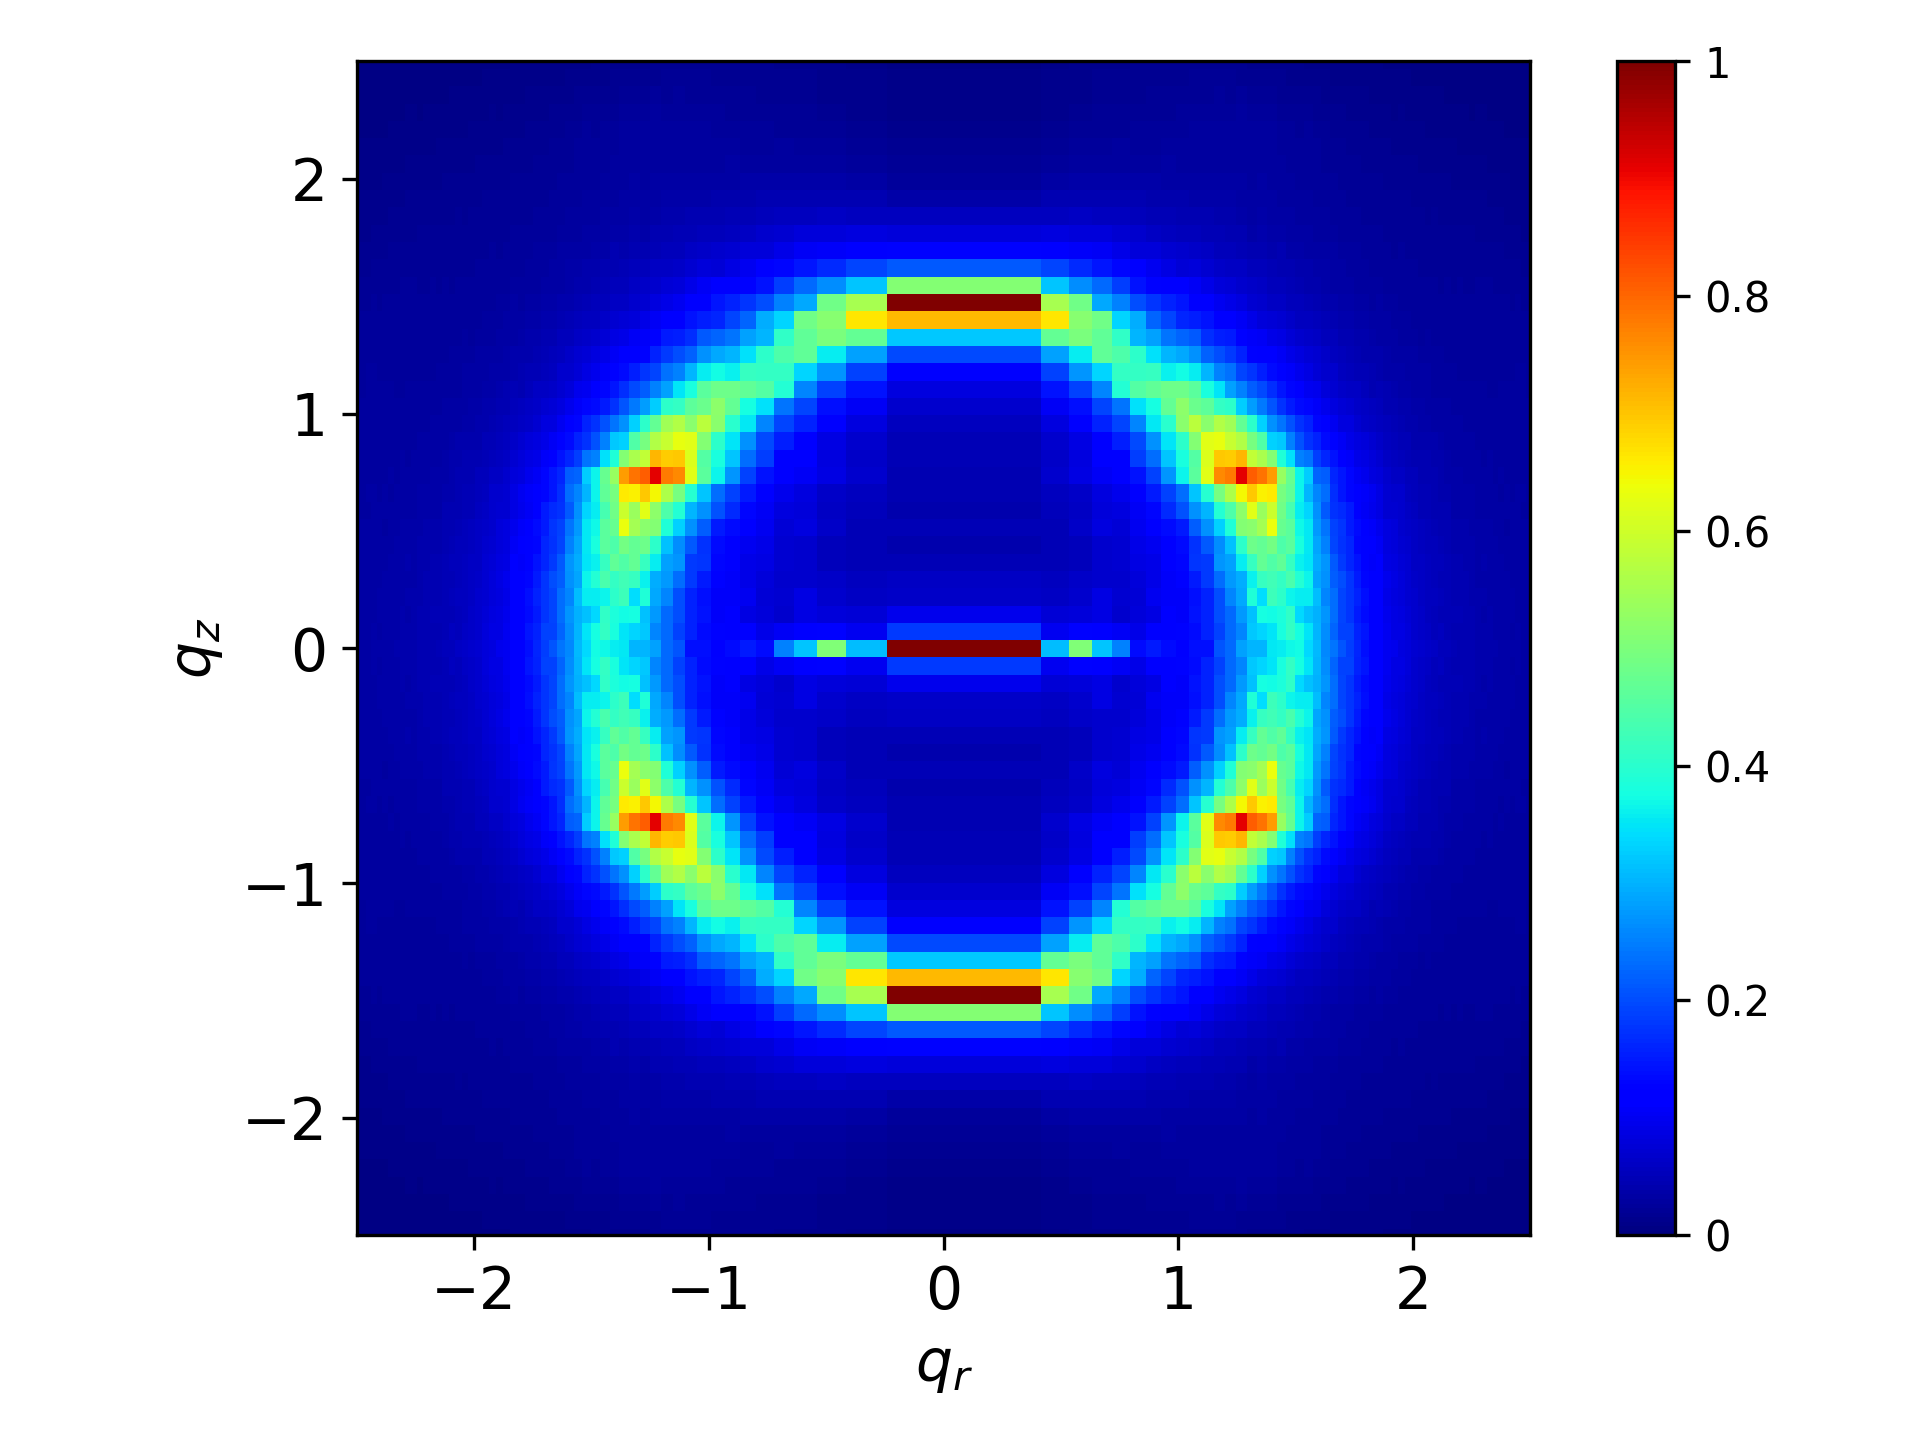
\includegraphics[width=\textwidth]{tails_rzplot.png}
		\caption{}\label{fig:tails_rzplot}
	\end{subfigure}
	\caption{(a) All atoms except carbon atoms making up the tails are removed from the 
	trajectory. (b) The simulated diffraction pattern of the tail-only trajectory still 
        shows R-spots}\label{fig:tails}
        %MRS2: might need to say how the dynamic range is adjusted here with only tails, since otherwise people will be confused with the R-spots being more intense. 
	%BJC: what do you mean by dynamic range?
	%BJC: Explain how colorbar is adjusted
  \end{figure}
 

  \begin{figure}
  \centering
  	\begin{subfigure}{\linewidth}
	\centering
		\begin{subfigure}{0.45\textwidth}
        		\centering
        		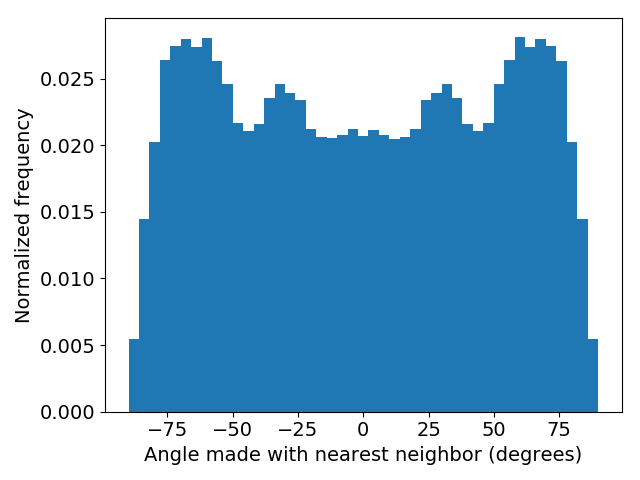
\includegraphics[width=\linewidth]{offset_tail_packing.png}
        		\caption{}~\label{fig:offset_tails}
		\end{subfigure}
		\begin{subfigure}{0.45\textwidth}
		\centering
	        	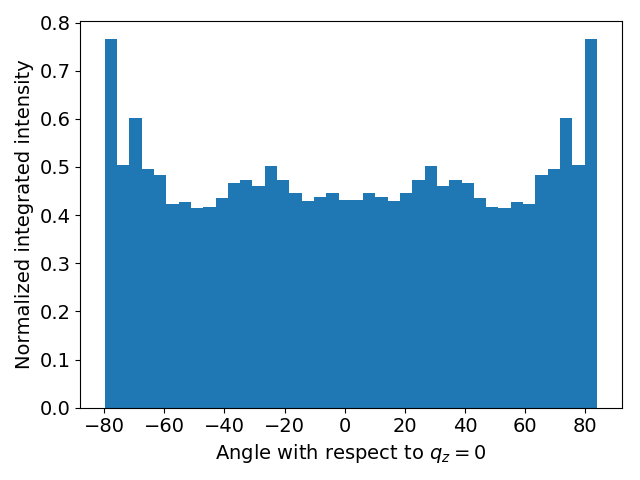
\includegraphics[width=\linewidth]{offset_angle_v_I.png}
		        \caption{}~\label{fig:offset_integration}
		\end{subfigure}
	\end{subfigure}
	\begin{subfigure}{\linewidth}
	\centering
		\begin{subfigure}{0.45\textwidth}
	        \centering
		        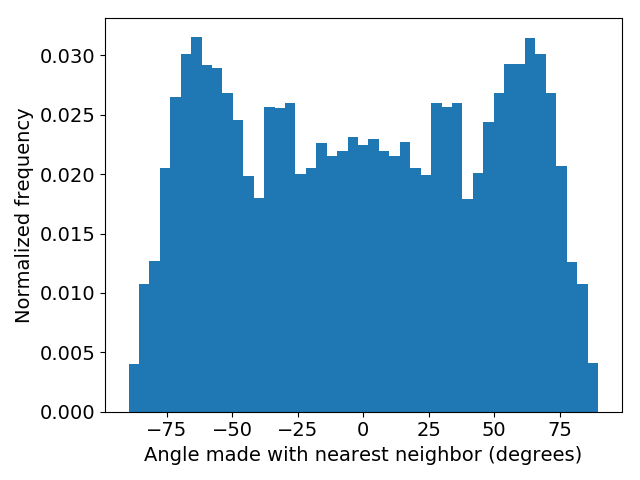
\includegraphics[width=\linewidth]{angles_traj_layered.png}
		        \caption{}~\label{fig:rz_layered}
		\end{subfigure}
		\begin{subfigure}{0.45\textwidth}
        	\centering
		        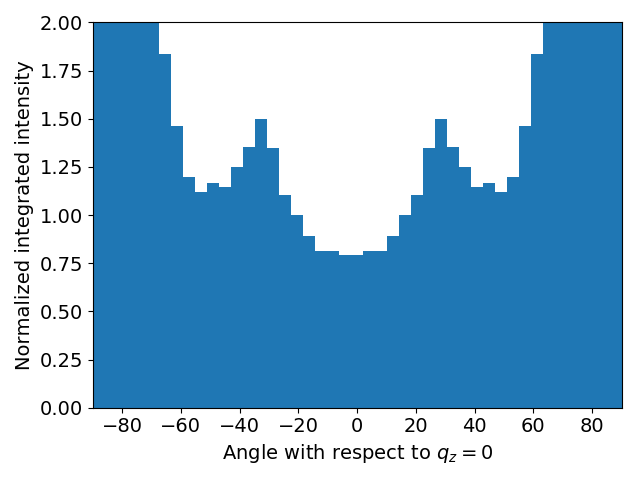
\includegraphics[width=\linewidth]{layered_angle_v_I.png}
		        \caption{}~\label{fig:layered_integration}
		\end{subfigure}
	\end{subfigure}
%MRS: 
  \caption{The distribution of angles w.r.t. the xy plane between alkane chain tail centroids and nearest
  neighbor centroids for equilibrated parallel displaced (a) and sandwiched (c) configurations. The
  same peaks are visible when the 2D simulated diffraction data is radially integrated in the R-alkanes region,
  (b) and (d) respectively.}~\label{fig:tail_packing}
  \end{figure}

%  The $z$-direction correlation functions show that layers in our model prefer
%  to stack further apart than 3.7 \angstrom as suggested by experiment.
  When systems are built with layers stacked 5.0 \angstrom apart then equilibrated, 
  we observe long-term stability of a qualitatively different configuration
  suggesting that we have found another metastable free energy basin,
  further corroborating \ref{point:metastable}. We studied this type of system in
  both the parallel displaced and sandwiched configurations. 

  Structural properties are different when layers are initially spaced 5 \AA apart.
  \begin{itemize}
	\item In both configurations we observe a decrease in pore spacing along with an increase in the equilibrated distance between layers.
	\item The simulated X-ray diffraction patterns differ particularly with reference to R-spots.
	\item R-helix is still faintly visible in the parallel displaced and absent in the sandwiched simulated diffraction pattern implying that head groups maintain their initial ordering to a degree.
	\item In both cases, R-spots is markedly different.
	\item When layers stack too far apart, they do not exhibit hexagonal packing
	\item The intensity within R-alkanes of the parallel displaced configuration is nearly uniform with slightly more concentrated intensity at the top and bottom.
	\item The sandwiched configuration possesses higher intensity regions at the top and bottom of R-alkanes as well as along the equator with high intensity near q$_z$ = 0.
  \end{itemize}

  \begin{figure}
        \centering
        \begin{subfigure}{0.45\linewidth}
                \centering
                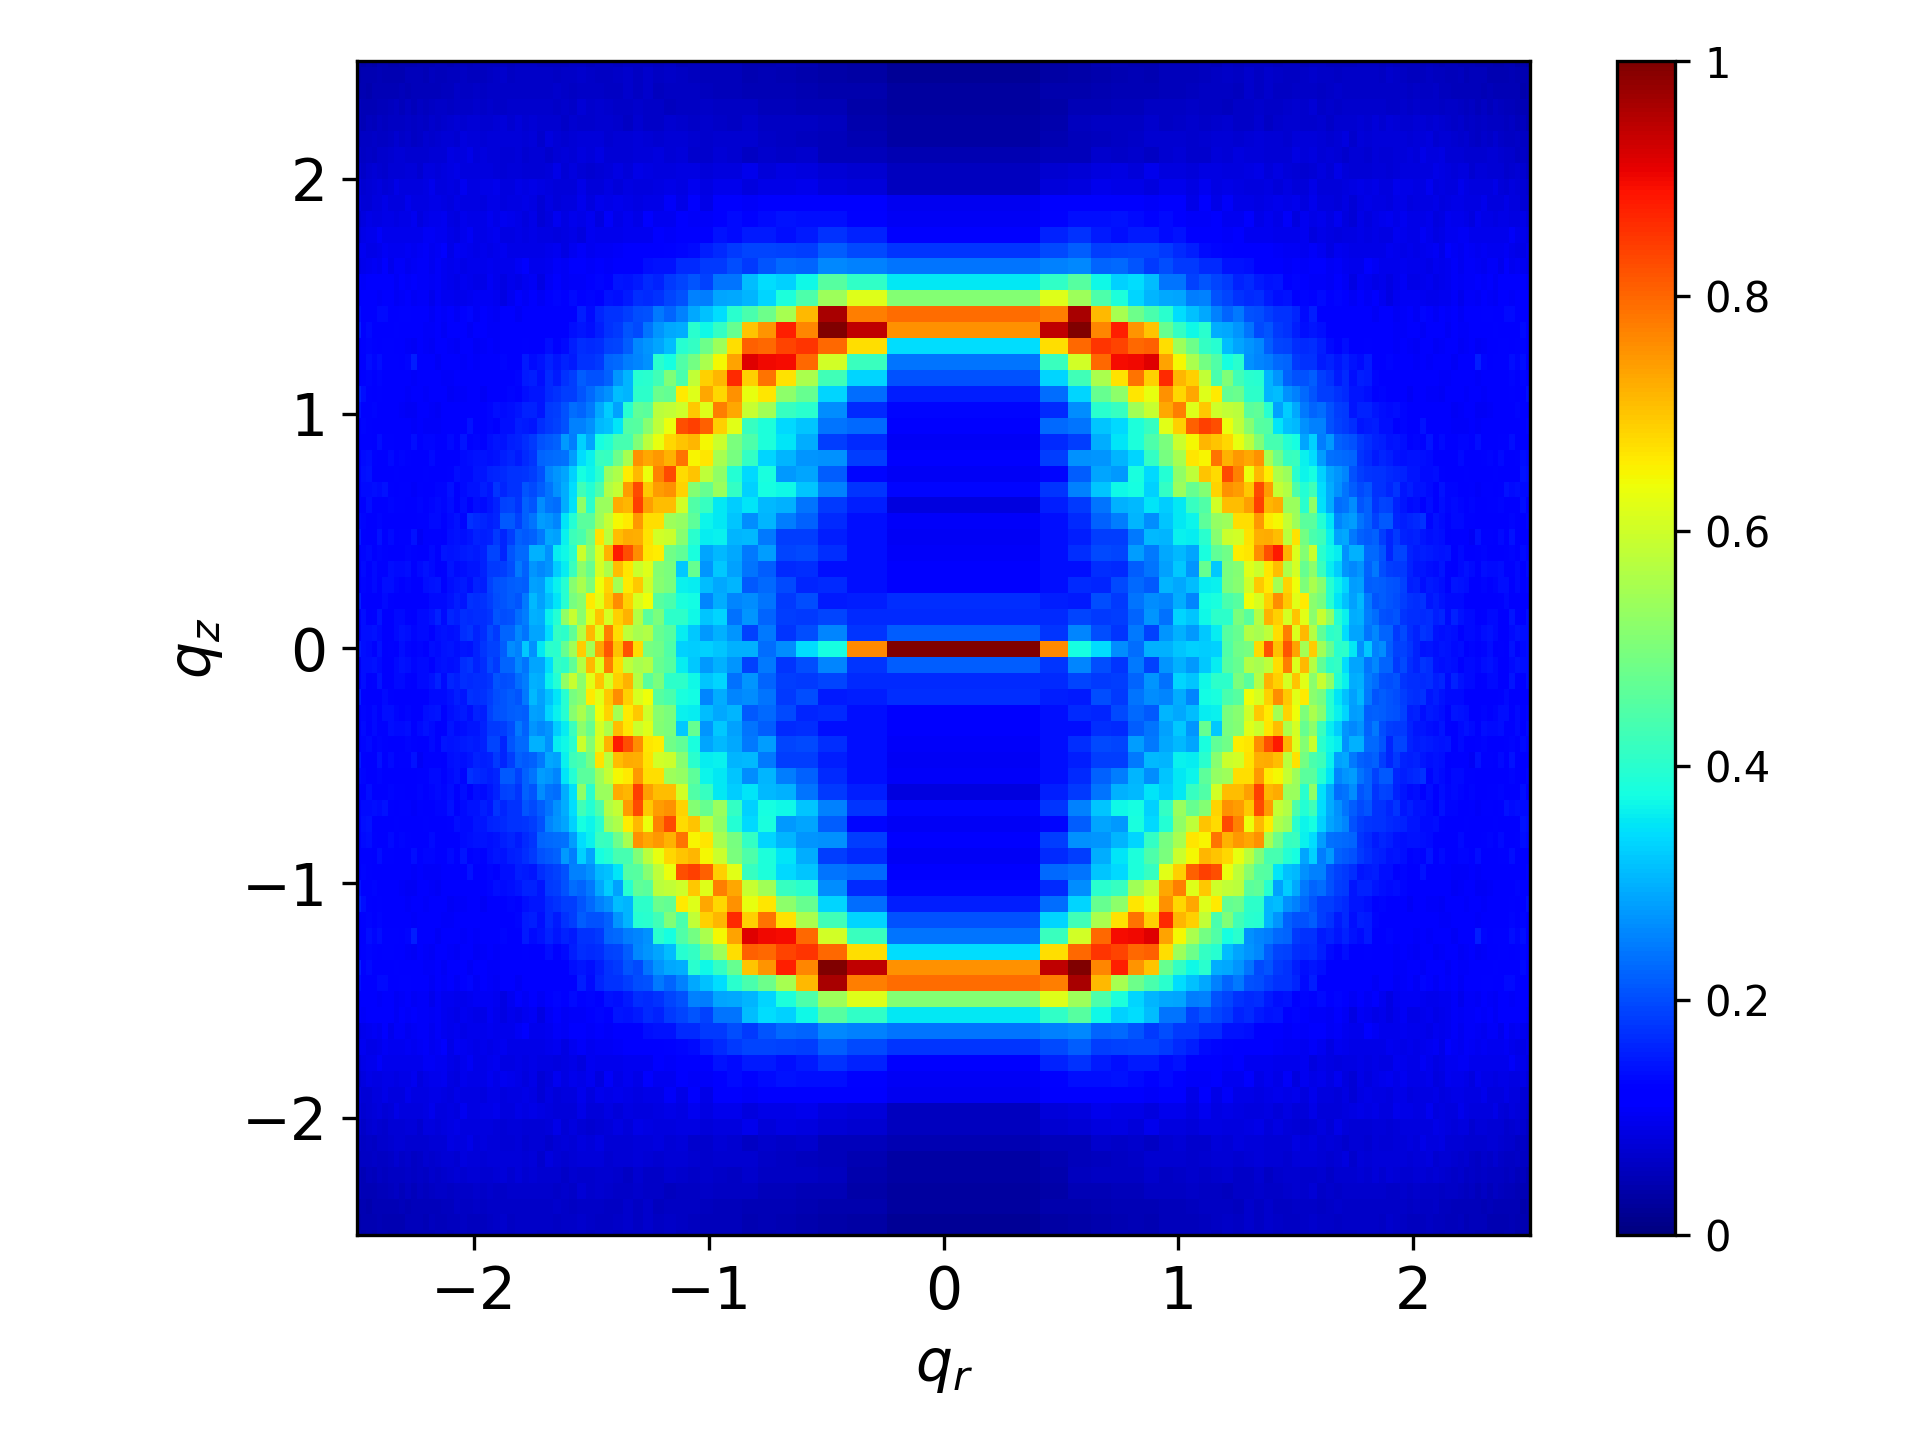
\includegraphics[width=\linewidth]{offset_disordered_rzplot.png}
                \caption{}~\label{fig:offset_disordered_xrd}
        \end{subfigure}%
        \begin{subfigure}{0.45\linewidth}
                \centering
                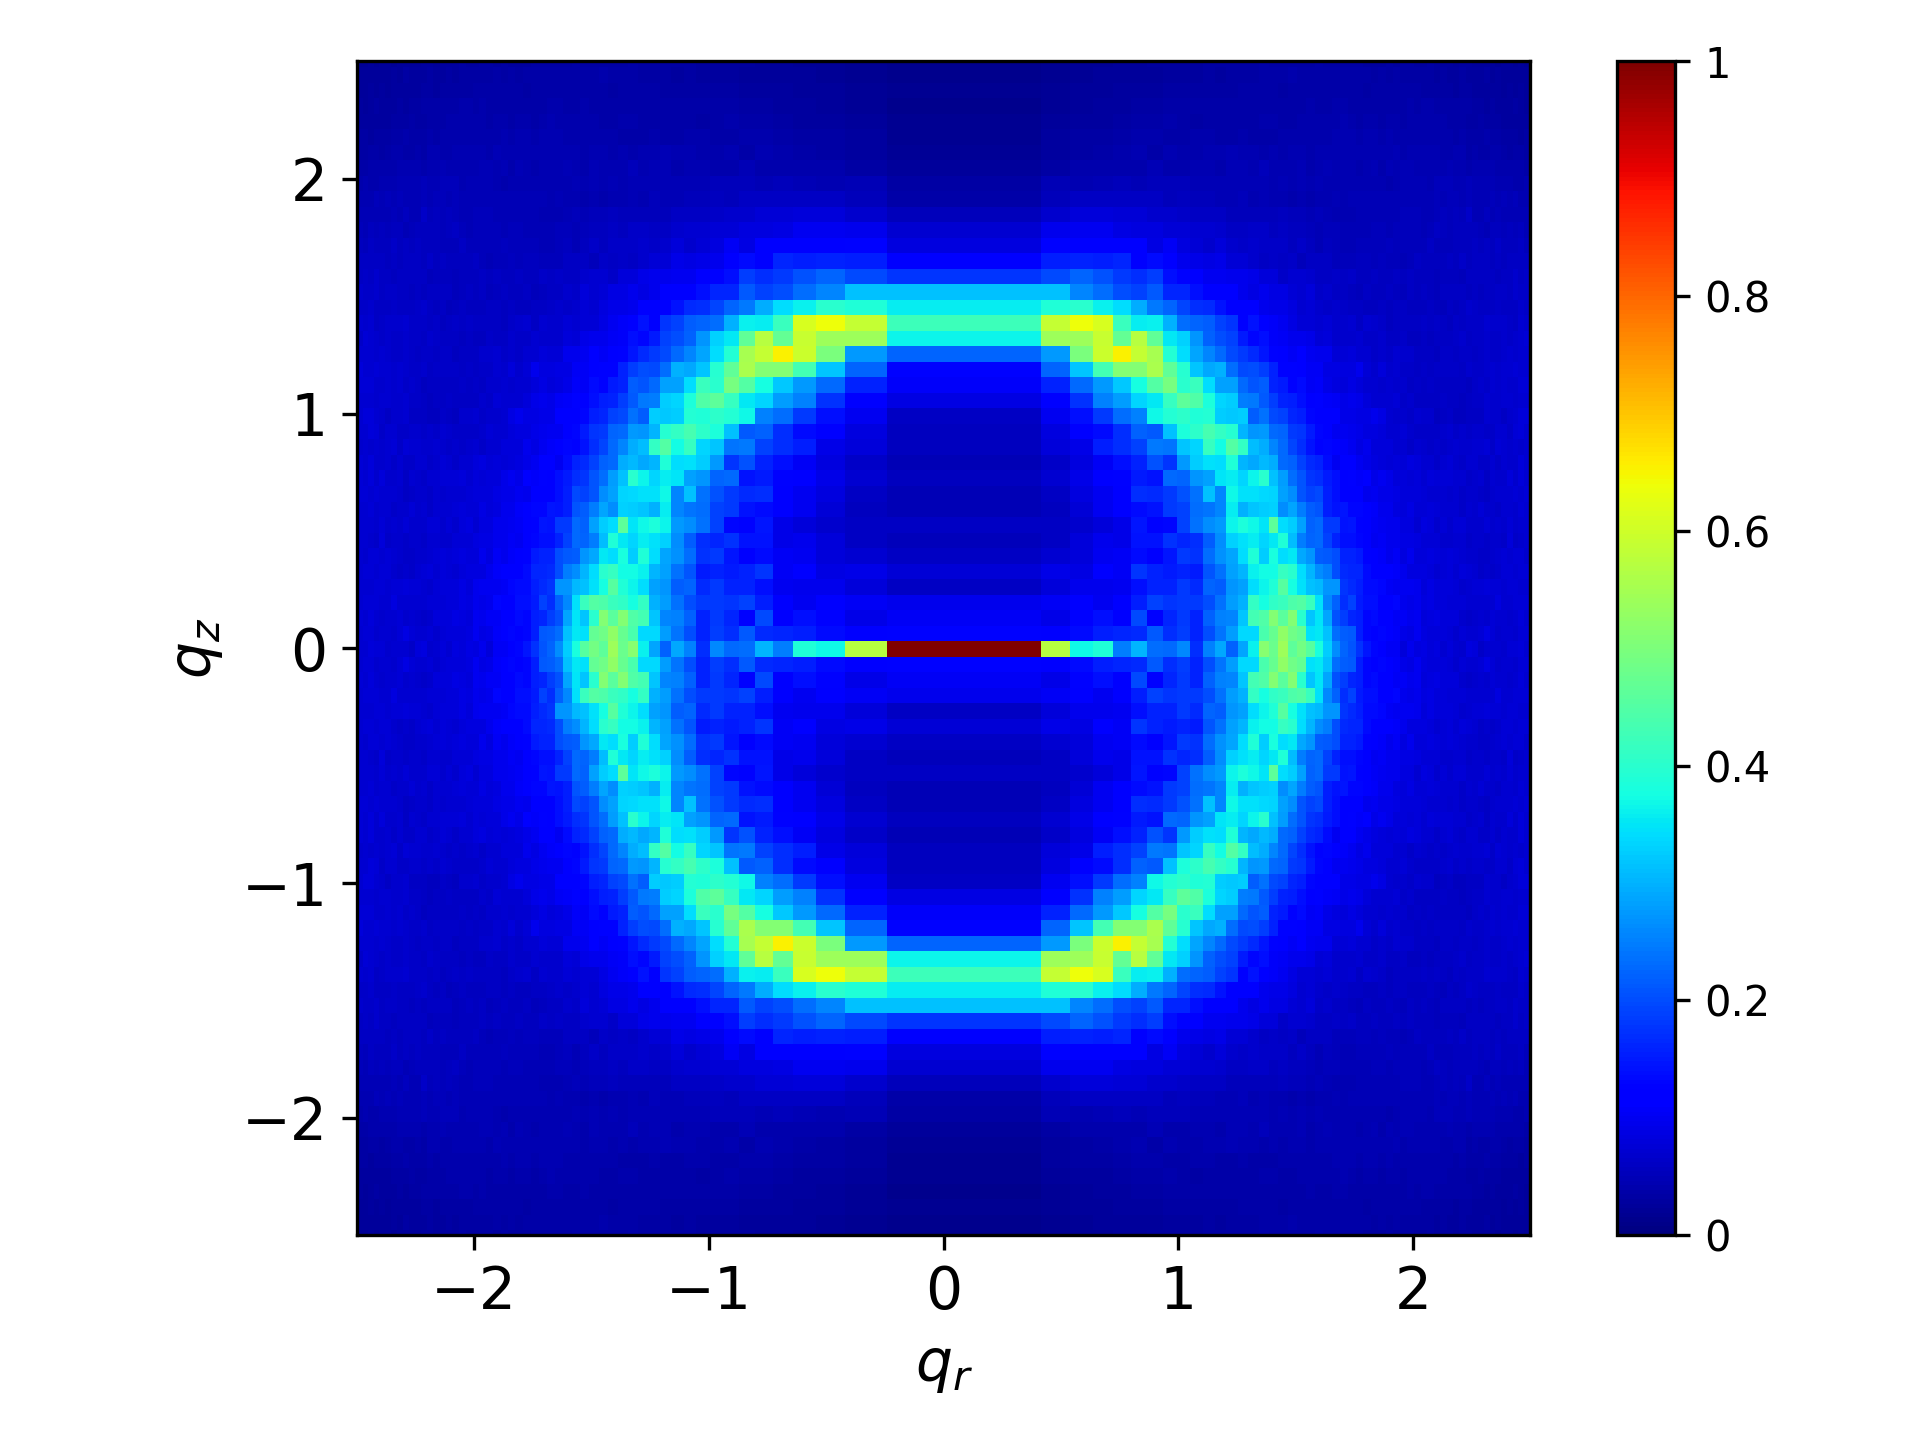
\includegraphics[width=\linewidth]{layered_disordered_rzplot.png}
                \caption{}~\label{fig:layered_disordered_xrd}
        \end{subfigure}
        \begin{subfigure}{0.45\linewidth}
                \centering
                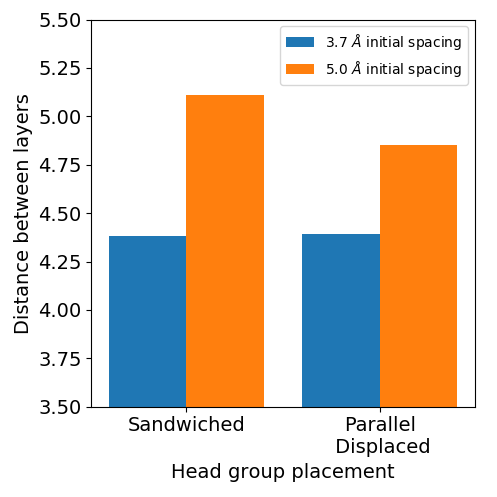
\includegraphics[width=\linewidth]{dbwl.png}
                \caption{}~\label{fig:dbwl_disordered}
        \end{subfigure}%
        \begin{subfigure}{0.45\linewidth}
                \centering
                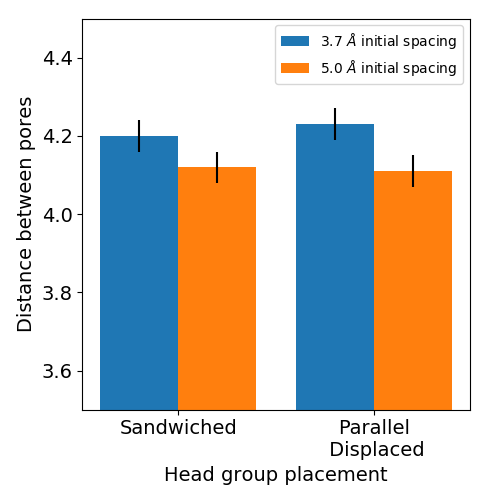
\includegraphics[width=\linewidth]{p2p2.png}
                \caption{}~\label{fig:p2p_disordered}
        \end{subfigure}
	\caption{In comparison to systems built with 3.7 \AA initial layer spacing,  
                the simulated X-ray diffraction patterns of the parrallel displaced (a) and 
 		sandwiched (b) configurations are different when systems are built with 
 		a 5 \AA initial layer spacing, most notably in the region bounded by R-alkanes.
      		When layers are stacked further apart, the distance between layers increases (c)
                and the pore spacing decreases (d).}
  \end{figure}

  In order to address \ref{point:poredefinition}, we plotted the number of
  densities of heavy atoms in the head group and tail regions of the monomers in
  addition to the sodium ions. (See Supplemental Information for definition of
  head group and tail regions). For the head group region, we used the carbon
  atoms making up the aromatic ring For the tail regions we used only carbon
  atoms of the monomer tails

  \begin{figure}
  \centering
  \begin{subfigure}{0.55\textwidth}
        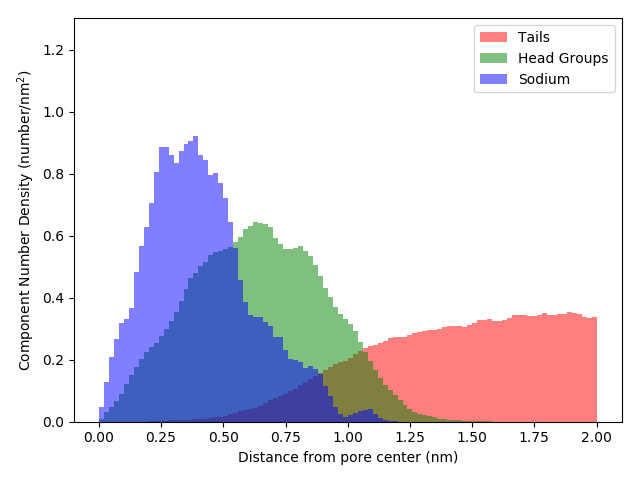
\includegraphics[width=1\linewidth]{offset_density.png}
        \caption{}
        \label{fig:offset_density}
  \end{subfigure}
  \begin{subfigure}{0.55\textwidth}
        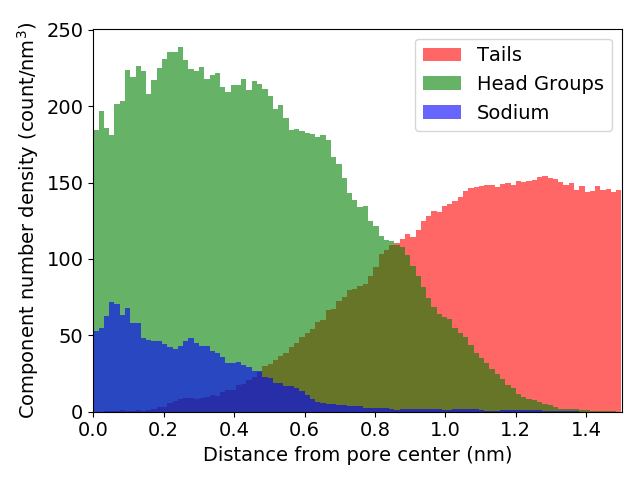
\includegraphics[width=1\linewidth]{layered_density.png}
        \caption{}
        \label{fig:offset_density}
  \end{subfigure}
  \begin{subfigure}{0.55\textwidth}
        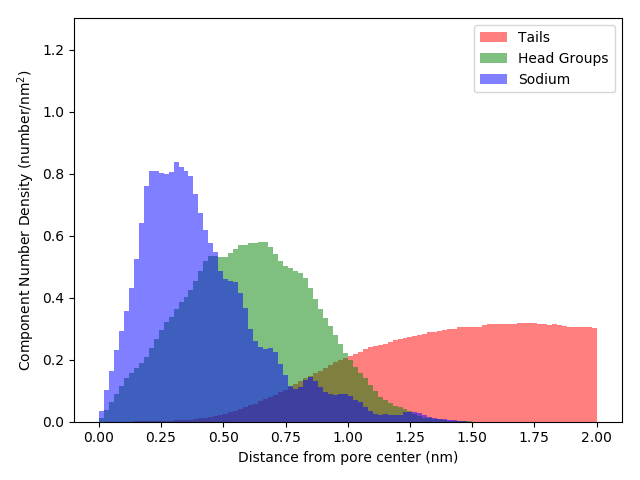
\includegraphics[width=1\linewidth]{disordered_density.png}
        \caption{}
        \label{fig:offset_density}
  \end{subfigure}
  \caption{(a) Parallel Displaced (b) Sandwiched (c) ``Disordered''}~\label{fig:densities}
  \end{figure}

  % BJC: necessary to show layered configurations at this point?
  We answered (\ref{point:water}) and further support (\ref{point:orientation})
  by preparing parallel displaced and sandwiched configurations according to the
  wet equilibration procedure. There is no experimental measurement of trace
  water concentration in the pores. We tested a range of water concentrations
  from 0.5 to 5 percent. Our lower bound models a system with on average 2 water
  molecules for each monomer layer. Figure ~\ref{fig:solvation} shows the
  simulated diffraction patters resulting from each configuration.

  \begin{figure}
	\centering
	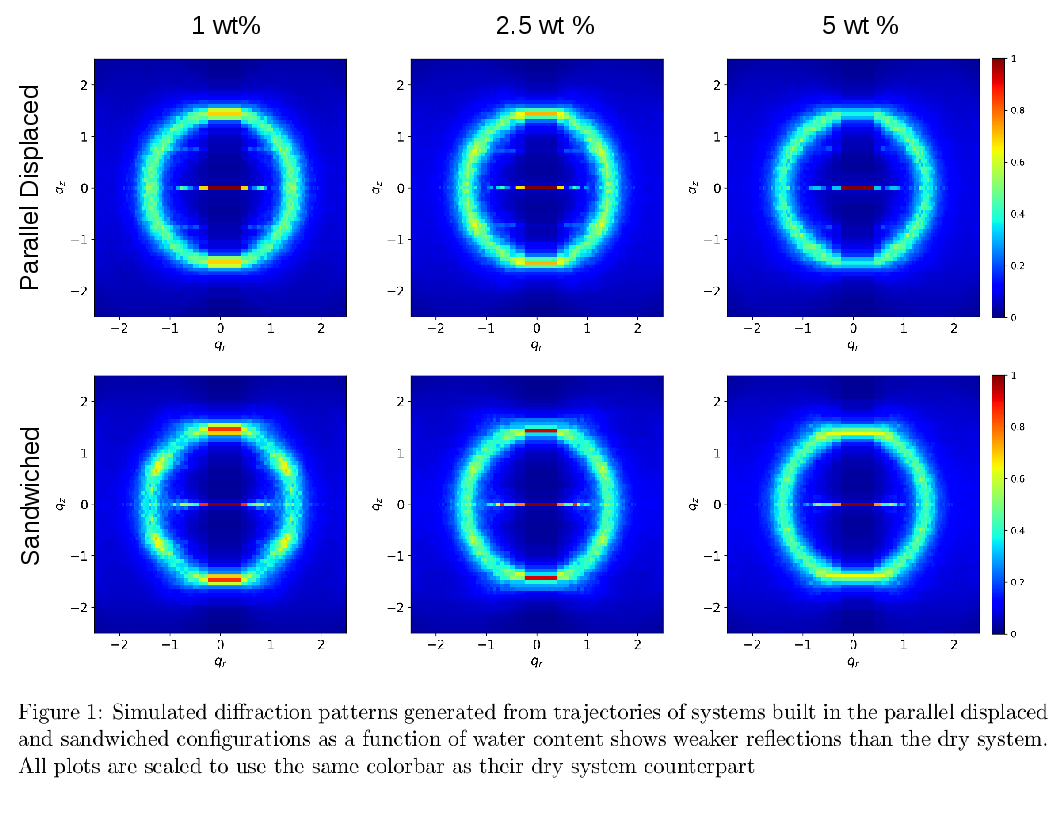
\includegraphics[width=\textwidth]{solvation.png}  % still working on formatting so this is a screenshot of a doctored latex figure
        %MRS2: include 0% as well? Maybe leave off 5% if not relevant in the end?
	\label{fig:solvation}
  \end{figure}

  In all cases, water disrupts structuring of the model. The plots in Figure
  ~\ref{fig:solvation} are normalized to have the same colorbar as the dry
  systems. The intensity of the reflections decrease when water is added to the
  system. In systems built with 5 weight percent water, R-$\pi$ and R-spots
  become nearly indistinguishable from R-alkanes.

%MRS3: is this point the right ``main'' thesis to make? I thought it was a more simple statement of being interested as to how water affected the structure.  FYI, would be interesting to see the RDF's of the pores with and without water, BUT I think that's not necessary for this paper, that's more a 2nd paper thing.
%MRS3: we didn't really test if water is  needed to obtain the structures; clearly, w/o water it's metastable for a long time.  We don't need the water simulations to prove this.  
  Water is not needed to obtain and simulate the correct equilibrium 
  membrane structure.
  \begin{itemize}
	\item We note that water absorbed during membrane synthesis may
        be present in far lower concentrations than those 
        tested here.
	\item We do not eliminate the possibility that water is necessary
        in order to drive self-assembly. Studying the mechanisms of self assembly is
	beyond the scope of this work.
	\item However, once the system has formed the Col\textsubscript{h} 
	phase, adding water only drives disorder in the structure
	\item In the equilibrium configuration, if water exists, it is confined
	to the pore region where there is no driving force for aggregation of 
	water molecules. 
	\item In the case of trace water, water molecules will be too sparse to
	form a hydrogen bonding network.
  \end{itemize}

  \subsection*{Ionic conductivity calculation}

  We use the equilibrated parallel displaced system to calculate ionic
  conductivity since its structure is the closest match to experiment. The model
  gives reasonable estimates of ionic conductivity when compared to experiment.
  Calculated values of ionic conductivity obtained using the Nernst Einstein
  relation and Collective Diffusion model are compared in
  Figure~\ref{fig:conductivity}. The two methods agree with each other within
  error, although the uncertainty obtained using the Collective Diffusion model
  is much higher. Much longer simulations are needed to lower the uncertainty,
  however it is not feasible to do so with a large system. We will only use the
  Nernst Einstein relation in future calculations of this type. 

  The calculated values of ionic conductivity are higher than experiment by an
  order of magnitude. One can justify the reason for this result by considering
  the real system studied experimentally. The ionic conductivity measurement to
  which we are comparing was done on a \SI{80}{\micro\metre} thick film, nearly
  10,000 times thicker than our simulated system. The thick film likely has
  defects leading to non-contiguous pores and imperfect alignment. The 2D SAXS
  pattern shows the small degree of tortuosity present in the system
  (~\ref{fig:2DSAXS}). It has been shown that there is a large dependence of
  ionic conductivity on the alignment of the pores. The ionic conductivity of an
  unaligned film is ca. 85 times lower than that of a nearly aligned film
  referenced here. We hypothesize that a thin, perfectly aligned film would have
  a value of ionic conductivity in agreement with our model

  \begin{figure}
        \centering
        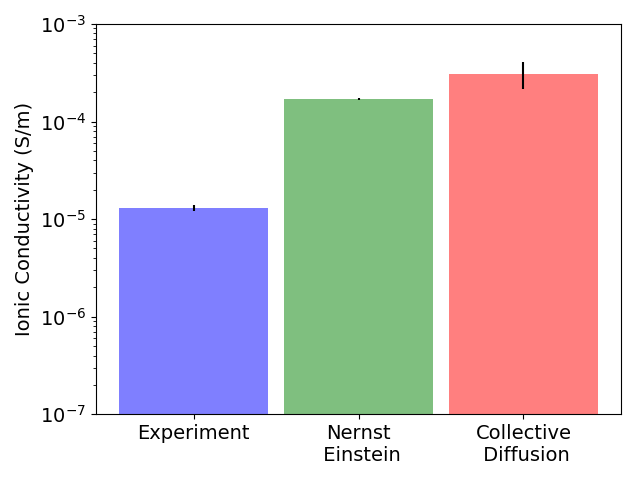
\includegraphics[width=0.5\linewidth]{IC_offset.png}
        \caption{Calculated ionic conductivity using the Nernst-Einstein relation
        and Collective Diffusion model agree with error. Both methods give calculated
        values of ionic conductivity an order of magnitude higher than the experimental
        value}
        \label{fig:conductivity}
  \end{figure}

  \begin{figure}
  \centering
  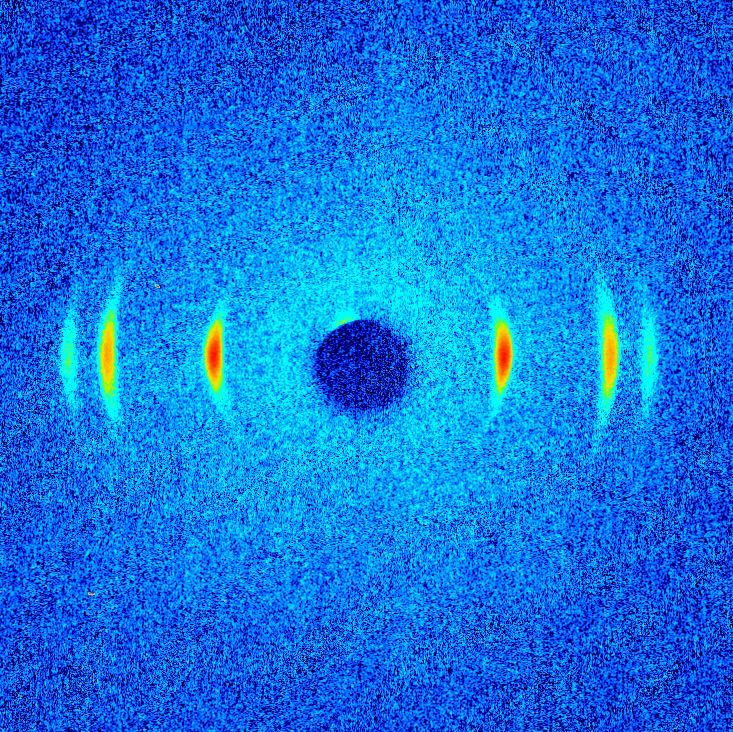
\includegraphics[width=0.5\linewidth]{2D-SAXS_cropped.png}
  \caption{Experiments confirm that the pores have a small degree of tortuosity. 
  The experimental two dimensional SAXS pattern exhibits reflections
  resulting from highly aligned pore regions. A perfectly aligned system 
  would exhibit sharp dots at the same locations of the refelctions shown. 
  An isotropically aligned system the reflections would appear as 
  rings centered about the origin}~\label{fig:2DSAXS}
  \end{figure}

  \subsection*{Implementation of the crosslinking algorithm}

  We applied the crosslinking algorithm to the equilibrated parallel-displaced  
  configuration with 5 monomers per layer.
  \begin{itemize}  %BJC: working on the following. The following is what I expect
%  	\item There is an even distribution of crosslinks between same monomer tails, 
%	between monomers in the same pore and between monomers in different pores 
%	including periodic boundaries.  % BJC: might leave this detail in the supplemental
	\item We reach 95 \% conversion of terminal vinyl groups % BJC: we'll see
	\item The distance between pores shrinks by 0.4\angstrom~ after the system is 
	crosslinked  
	\item We simulated the crosslinked system in the NPT ensemble for 100 ns
	\item Major features are still present in the X-ray diffraction, however at lower intensities ~\ref{fig:rzplot_xlink} 
	\item The ionic conductivity is lower in the crosslinked system ~\ref{fig:ic_xlink} % BJC: Nernst-Einstein is lower. Need a longer simulation to check Collective-Diffusion - I can probably avoid that by saying that we will be sticking with the Nernst-Einstein method
  \end{itemize}
 
  \begin{figure}
  \centering
  \begin{subfigure}{0.45\textwidth}
	\centering
	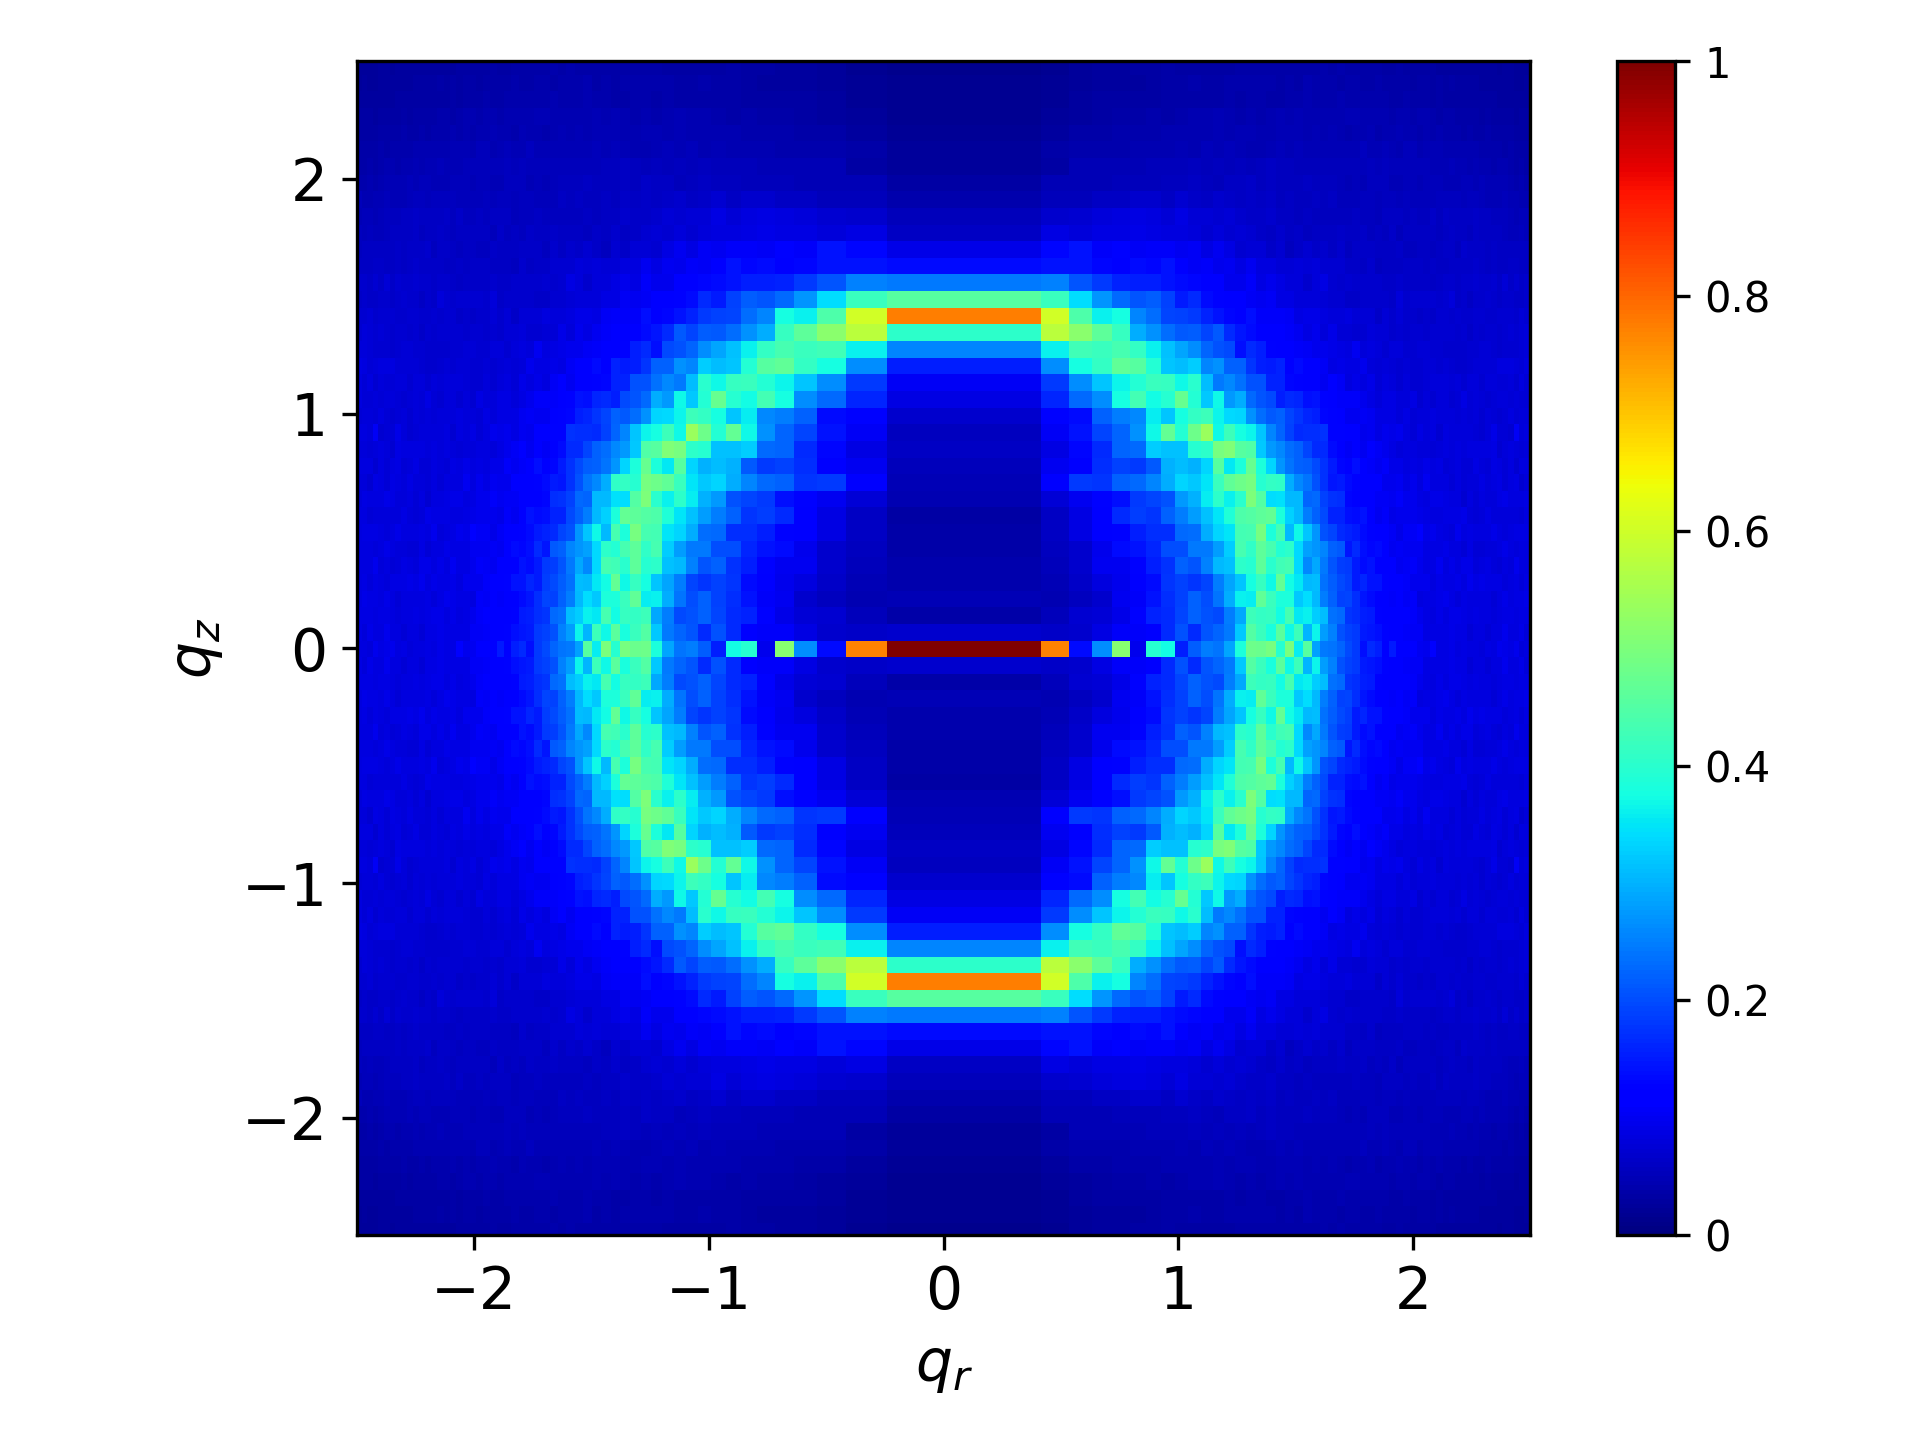
\includegraphics[width=\textwidth]{rzplot_xlink.png}
	\caption{}~\label{fig:rzplot_xlink}
  \end{subfigure}
  \begin{subfigure}{0.45\textwidth}
	\centering
	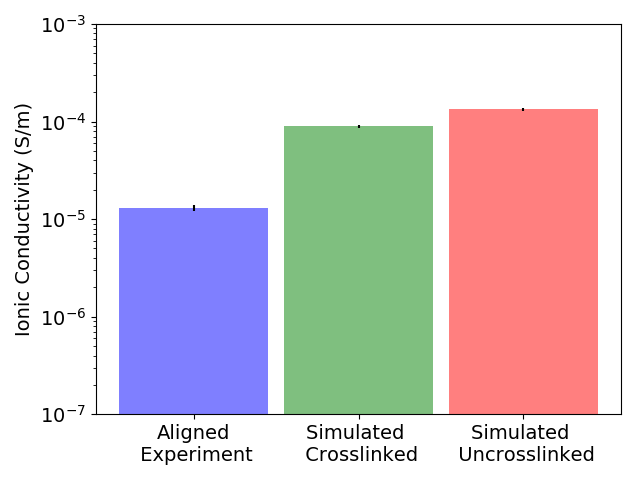
\includegraphics[width=\textwidth]{ic_xlink.png}
	\caption{}~\label{fig:ic_xlink}
  \end{subfigure}
  \caption{(a) Reflections produced by the crosslinked configuration fade relative
  to the uncrosslinked system. The colorbar shown is the same used for the uncrosslinked
  system. (b) The ionic conductivity is smaller relative to the uncrosslinked system, but
  still much larger than the experimental value}~\label{fig:xlink}
  \end{figure}
 
  \section*{Conclusion}
  
  % add stuff about pore structure and 'disordered' basin once there are concrete results 
  We have used a detailed molecular model of the Col\textsubscript{h} phase
  formed by NA-GA3C11 in order to study its nanoscopic structure. While there
  have been efforts to model formation of various liquid crystalline phases with
  molecular dynamics, to our knowledge there have been no studies which attempt
  to examine their structure with the same level of detail presented here.
  Evidence strongly supports that layers are composed of 5 monomers. We have
  confirmed that monomers stay partitioned into layers. We have explored the
  affect of two different $\pi$-$\pi$ stacking modes on the equilibrated membrane
  strucure. Simulated diffration patterns generated from MD trajectories suggest
  that the parallel-displaced configuration produces a structure with the closest
  match to experiment. Finally, water is not needed to create well-definied pore
  structures. Now that we have a good idea of what the membrane structure should
  look like, we will evaluate transport of various solutes within the system. We
  will apply the knowledge gained from this study in order to suggest
  improvements to the existing system as well as to evaluate new unsynthesized
  LLC systems.

  \clearpage
  \bibliography{llc}

\end{document}
